% intro %

\section{intro}

ECAL performance is crucial for	precision measurements that involve electrons and photons. (add examples) 
Also for the reconstruction of the jets	and missing transverse energies	(this should be showed in PF section)

as mentioned previosuly ECAL is designed to measure the energy deposited by electrons and photons. 
These particles deposit thier energy in ECAL by showering in the ECAL crystals.

%... details about the crystals arragement in the ECAL ... % 
%ECAL made of a barrel region and two endcaps. EB has 36 supermodel, quarter EB has 9 supermodels facing the beam line.
%each super model has about 1700 crystal coverting eta 0-1.48 and deltaphi 0.35. each crystal depth is 23cm in the EB.
%(here insert picture shows eacl regions https://indico.tlabs.ac.za/event/112/contributions/3216/attachments/1138/1538/TIPP2023-Dimova_v1.pdf pg 4 2 figures)
%(for more detailed skitch of each supermodel and trigger towers https://www.researchgate.net/figure/Top-panel-physical-view-of-an-ECAL-supermodule-in-the-CERN-SPS-H4-beamline-where-the_fig2_4291336)
%(real picture of endcap crystals https://cds.cern.ch/record/1100782)
%(picture of ECAL supermodels during cosmic ray testing https://cds.cern.ch/record/1431477?ln=en)
%(picture of crystals and number of types in each regions pg 5 tapered means shaped https://indico.tlabs.ac.za/event/112/contributions/3216/attachments/1138/1538/TIPP2023-Dimova_v1.pdf) 

EM showers spread over multiple crystals (small Molière radius 2.19 cm while crystal transverse size is close 2.6 cm)
clusters are extended in phi direction to form "superclusters" to recover energy radiated via bremsshtrahlung or conversion.
(inster picture shows how the superclusters could look like pg 6 https://indico.tlabs.ac.za/event/112/contributions/3216/attachments/1138/1538/TIPP2023-Dimova_v1.pdf)

to get the correct energy for a photon we generally include corrections that was done perfore data taking and other in situ.
(include equation) 

These corrections include: intercalibration (equalize signal response for the same eta)
%(check pg 4 skitch for one supermodel https://indico.tlabs.ac.za/event/112/contributions/3216/attachments/1138/1538/TIPP2023-Dimova_v1.pdf)  
Also laser corrections for signal transparency loss (or photocathode aging) (this calibration is done every 40 mins),
cluster correction obtained from a regression method. (this is what this thesis is focused on)


the material in front of the ECAL and dead material in ECLA effect the deposited energy so we apply the following corrections:
corrections applied to reconstruct the original deposited energy of the particle (our focus)
after this correction we need to do an a scale energy correction in data to match the simulation.
% ^ more details check paper https://iopscience.iop.org/article/10.1088/1748-0221/16/05/P05014/pdf 


% check reading notes to introduce the subject.

The reconstructed PF cluster energy is expected to be smaller than the energy of the incoming particle.
This lost of energy could be due to tracker material, gaps, dead channels etc. Therefore, a clibration of the calorimeter cluster energy is needed. 
% The PF ECAL cluster calibration, which is supposed to account for the effects of these thresholds,is determined from simulated diphoton gun samples
% ^ source: PF paper 

(this into need to be connected with PF cluster calibration, do quick mention to it)
(fix intro after finishing this chapter) 

This chapter presents the used ML method and datasets in performaing the PF ECAL cluster calibration.  
% check https://par.nsf.gov/servlets/purl/10421786 for intro / source about EM calibration. 
%.................................        

\section{data sets description}
%(check reading notes)

%dataset=/DoublePhoton*FlatPT*13p6TeV/Run3Winter24MiniAOD*NoMaterial*/MINIAODSIM
%15 dataset pt ranges: 1-10 (3  datasets) , 1000-1500 (3 datasets), 10-500 (3 datasets), 500-1000 (3 datasets)
%each group of dataset has: PU 0-120, 0-80, No PU
%each dataset (of specific pt range, PU type)  has multiple root files that contains number of events. 

% instructions for calibration ntuple production https://codimd.web.cern.ch/IwKw1T6VQw6Q8mHpvK3Mzw
% updated the list of the input files
% used cmsRun runAnalyzer.py to produce the ntuple.


The dataset samples used in this calibration are Double photon with no material produced centrally under CMSSW 13_3_0.
% using particle gun sample (double photon) without any material up stream of the calorimeter
( note: after producing	the calibration	ntuples	we concatenate them into one file for each pt bin separately for noPU and PU) 

The training and validation was done under CMSSW 10_5_0.
% instruction for training and validation https://codimd.web.cern.ch/kTx6DIOYQ_qL4mpJE_H6fA

(note: we separate the each data sample into two. one for training and another one for testing.)

(note: after that we split the training sample to different regions of the ECAL (barrel, endcap))

(note: also we split each region into two categories: Full readout (3 groups) , zero suppression readout (1 group))

% full readout refers to recording data from every crystal in ECAL regardless of the energy deposit.
% zero suppression refers to only reading out data from crysta;s that exceed a certaing energy threshold
% ^ chech source: https://arxiv.org/pdf/1806.09136#:~:text=Upon%20L1A%20signal%20these%20flags,time%20samples%20without%20any%20suppression. pg 4 

% or check source that has picture of the readout https://ieeexplore.ieee.org/stamp/stamp.jsp?tp=&arnumber=1462385 or https://cds.cern.ch/record/687490/files/note03_001.pdf
after preparing the appropriate date sets. Training is done only on no PU samples.

The testing is done on both no PU and PU80. 

(note: check ths statistics used for each case Full pT1/ Full pT2/ Full pT3/ ZS for both EE, EB)

% Ntuples are simple data tables generally containing simple float quantities. Very compact, these are the files that we usually use in the interactive analysis.
% ^ source: https://oer.uclouvain.be/jspui/bitstream/20.500.12279/398/1/LPHY2131_Documentation.pdf

%................................. 
% check https://cms-opendata-guide.web.cern.ch/tools/root/ has ROOT tutorials. 
% Also https://root.cern/doc/v628/group__tutorial__tree.html ROOT tutorials
% https://github.com/cms-opendata-analyses/JetNtupleProducerTool HEP exploring ntuple 

\section{PF cluster regression using BDT}

PF cluster regression used to correct for PF cluster energies lost due to tracker material, gaps, dead channels etc.

PF cluster regression is a BDT based semi-parameteric regression. 

To estimate the correction. it is useful to take the PFcluster where a photon has deposited all its energy in one PFcluster.

then correction for the PF cluster = Egen_photon/Eraw_pfcluster.

we are going to use only "no material double photon particle gun" samples.

%This regression is used by JetMET group.
% ^ JetMET is responsible for monitoring, reconstructing, calibrating, and providing scale factors and software tools for jets and missing energy in CMS.

training is done on no PU samples as seen before this same gives better training comparing to PU samples. 


We are adopting the same variables used previously in Run 2 & Run 3 (2023). The PF cluster regression is done intro two steps:

1) Training (from where we will get trained regression model).
2) The validation of the training is done on NOPU and PU(80) samples.

% check source for ML and BDT for ECAL  : https://cds.cern.ch/record/2702355/files/1911.02501.pdf 
%.................................    

\subsection{BDT}
%(explain how BDT work in general)

(Decision tree): is a tool that could be used to divide the data into simple regions in order to classify or regress the inputs.

In (regression tasks): the model predicts the numerical value of the target.

ML method based on decision trees uses a loarge number of these trees to classify or regress to a true output.

boosted decision trees (BDTs) : when the outputs of the trees in the method are dependent on one another.

types of boosting available to BDTs: adative boosting (adaBoost), gradient boosting, extreme gradient boosting (XGBoost) which is what is implemented here. 
(quickly methioned the difference between them. 
% finished DT, adaboost tutorial 

Gradient boosting (GB): based on popular optimization technique called gradient descent algorithm.
same concept but instead of minimizing the output function, it minimize the error function/ loss in the direction of the process.

learning rate: the size of the steps of the gradient descent.
error/residual of the decision making: true output - prediction made by the model.

New prediction (GB)  = old prediction + learning rate * residual. <= this shows that the total predictive model is just a collection of all trees in the model.

Extreme Gradient boosting (XGB): is an advance version of the GB. to avoid the overfitting penalty terms are added to the residual of GB.

New prediction (XGB) = old prediction (GB) + penalty * residual(branch) = mean/median of the error of the current branch.



\subsection{input features}
The training input variables include independent variables (features) used in the training:

clusrawE,
ieta,iphi (EB) ,
ix, iy (EE),
ietamod20, iphimod20 (EB only),
(clusPS1+clusPS2)/clusrawE (EE only),
% ^ (ratio of preshower energy to the clusrawE for EE)
% source : https://baylor.app.box.com/file/1664942425535 
number of hits in the cluster (which takes values 1, 2 and 3 - it takes 3 if nhits >= 3).
% ^ which make it less dependent on the # of actual hits in the PF cluster.
% since the correction is finally to be applied on the jets
% source: PF clusters training for 2017 UL (2019) https://indico.cern.ch/event/823872/contributions/3458420/attachments/1857689/3060324/egmpfcluster_regression_5june.pdf
% source : PF clusters training for 2017 UL (2017)https://indico.cern.ch/event/646805/contributions/2627253/attachments/1477404/2289247/status_regression_15june.pdf 
% source : details about the vairables https://cds.cern.ch/record/2702355/files/1911.02501.pdf

Also  used Target: log(Egen/Eraw).

\subsection{training}
Training is done on no PU Zero material double photon particle gun. During training we are going to adopt the same variables used in Run 2 calibration for Run 3 (2024).

The ML method implemented for PF ECAL cluster calibration is a Boosted Decision Tree (BDT) based semi-parametric regression.

To estimate the correction to  the PF ECAL Cluster, we consider the case where a one photon has deposited all its energy in one PF cluster in the ECAL.
This will allow us to calculate: the correction factor = E “gen photon” / E “raw pf cluster”.

% note: calibration under CMSSW 12_0_2 derived under 2022 MC conditions (ankush) 
% ^ this is same as making ntuples for the PF cluster regression ----- for Run 3 V0 under 12_0_2 (in das 120X) 
% Re calibration in CMSSW 12_6_3 in another darsets produced using 126X .. in das shows 126X (mine was 133X)

Training conditions:
Trained for zero-suppressed and full readout regions separately.
(For full readout, three regressions are trained:raw pt [5, 20], [20, 100], and [100, 300] GeV)
Total of 8 regressions were trained.

\subsection{performance and validation}
The validation is done through few steps.
First from the training model we get the value of the correction factor, then  calculated:  the corrected cluster energy = E “raw pf cluster” * correction factor

Plot: the response: E “corrected PF cluster” / E “gen photon”
Fit the plot with: double CB function. ( for pt< 6 GeV we use Gaus function for fitting since it will be difficult to do the with double CB- in other words low pt (zero suppressed)) ) 
From the fitted curve we find: mean, effective sigma.We can also get the mean, effective sigma for raw PF cluster energy “with no correction” to compare.

% source: twiki page https://twiki.cern.ch/twiki/bin/viewauth/CMS/EGMPFClusterRegression 
\section{results}

The presented plots show a comparison between the calibration results of the new (presented) corrected ECAL cluster in 133X (blue line), to the current (previosu)  correction in 126X (green) and  raw PF ECAL cluster (red).

generally we see that the new correction very close to the current used calibration

Usually, the since the PF clustering is performed separately in each region of the ECAL: ECAL Barrel (EB), ECAL Endcaps (EE).
Presenting the results in a similar way.

Overview of the results: we checked the 2024 double photon calibration samples for PF ECAL clusters.

In general, the existing calibration derived from 2022 samples seems to continue to be working well.

% check % source: PF clusters training for 2017 UL (2019) https://indico.cern.ch/event/823872/contributions/3458420/attachments/1857689/3060324/egmpfcluster_regression_5june.pdf
% ^ to see how the plots were analyxed
% we could also comapre the resuls for PU and noPU check comments (2021)  https://baylor.app.box.com/file/1664940788584

(note: add comment about future calibration for ECAL PF cluster)

\subsection{ECAL Barrel}
first starting with the NOPU sample then the PU case.
plots show response (resolution) vs Pt gen in GeV and in their corresponding eta range.
\begin{figure}
\includegraphics[width=0.495\textwidth]{./plots_pdf/ECAL_plots/plotsPU/EB/FULL/pdf/GENPT/EBFULL_GENPT_0005_0020_MuOverBins.pdf}
\includegraphics[width=0.495\textwidth]{./plots_pdf/ECAL_plots/plotsPU/EB/FULL/pdf/GENPT/EBFULL_GENPT_0005_0020_EffSigmaOverBins.pdf}
%\caption{EB - Full Readout pt 5-20}
%\end{figure}
%\begin{figure}
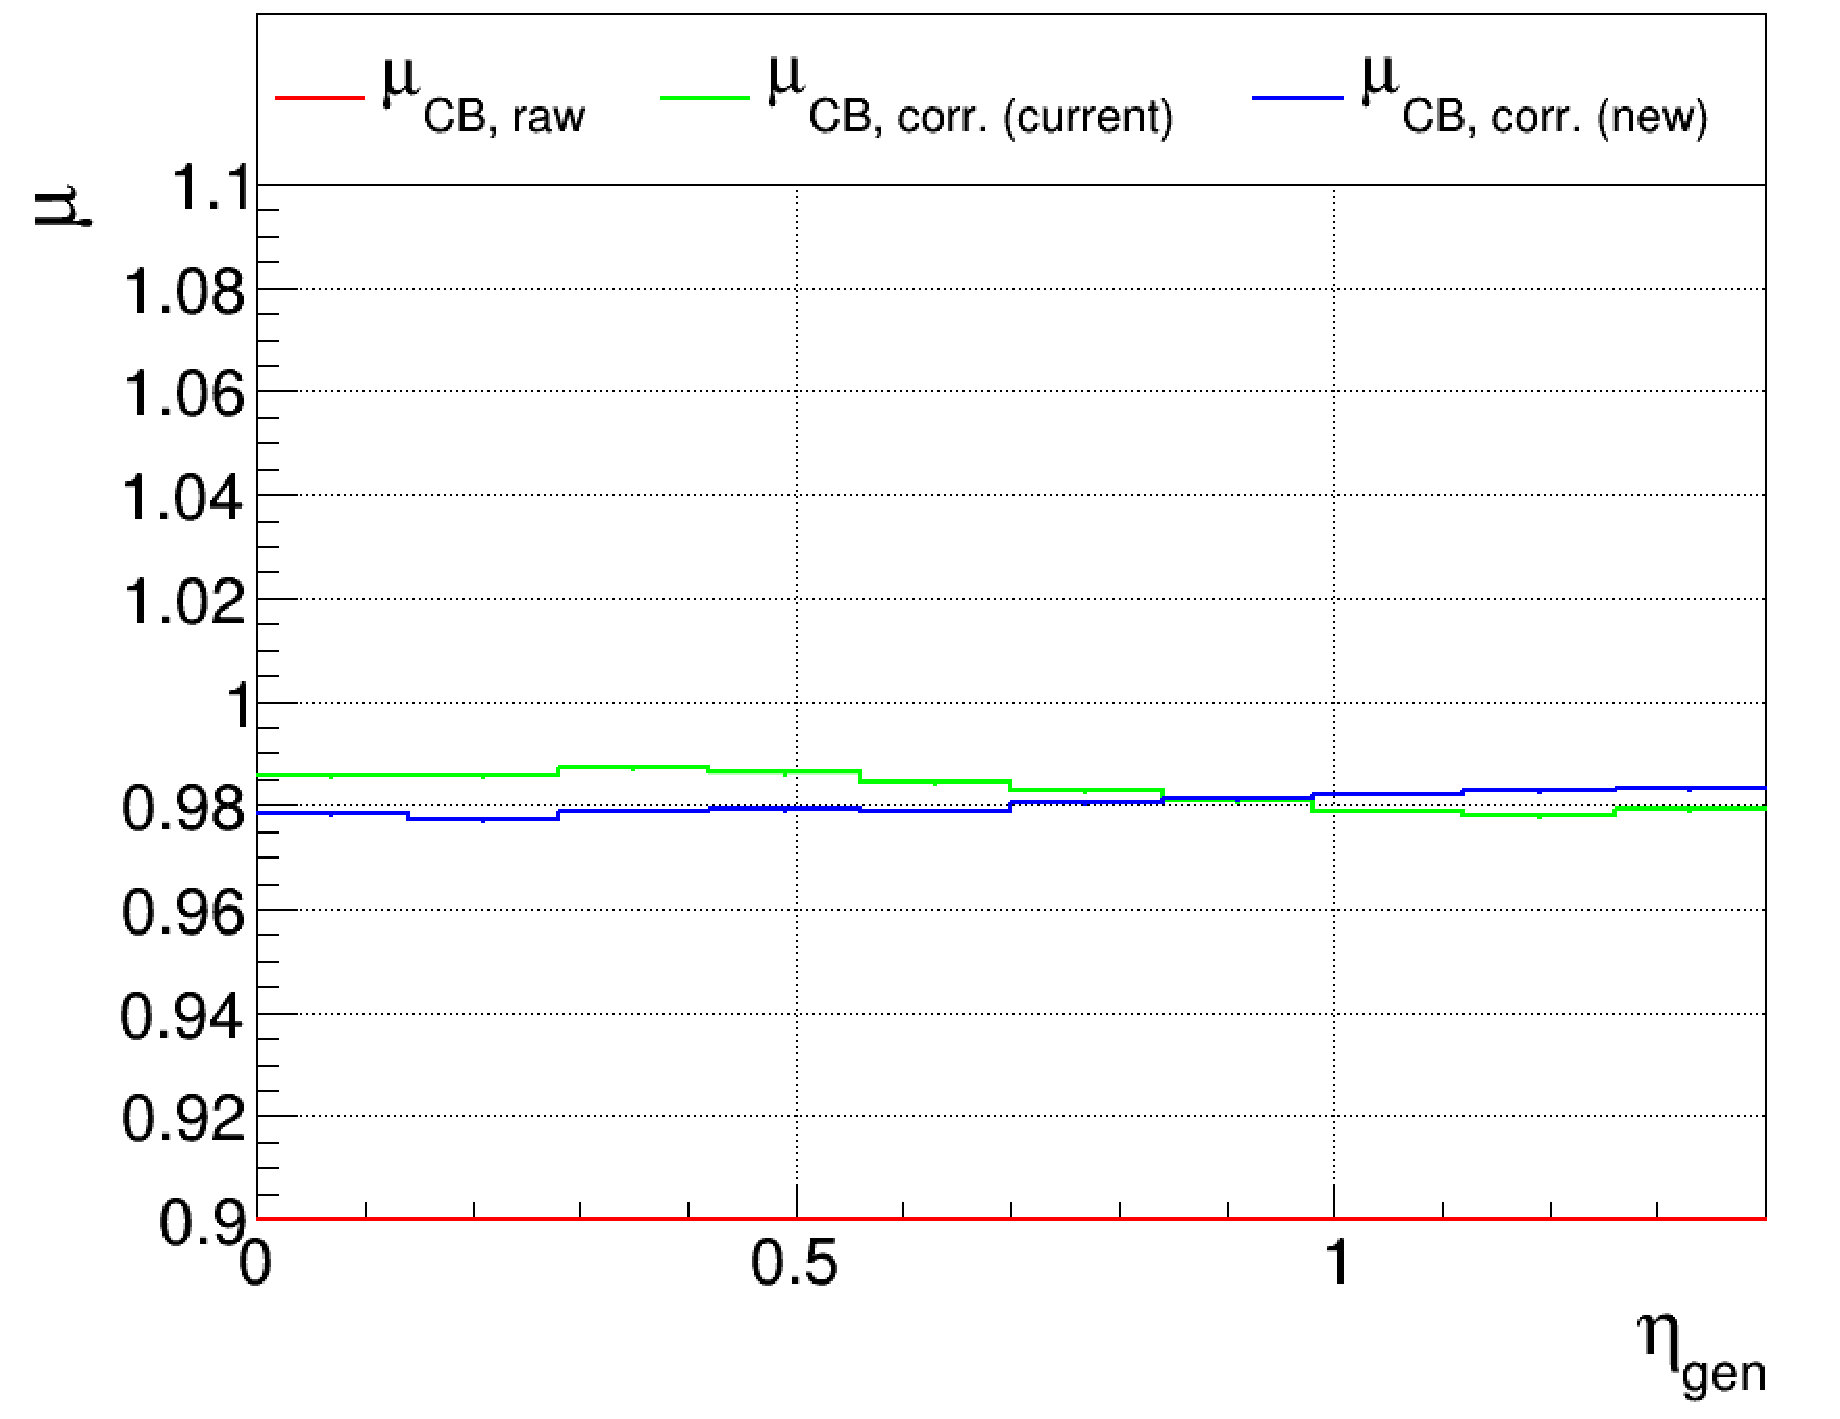
\includegraphics[width=0.495\textwidth]{./plots_pdf/ECAL_plots/plotsPU/EB/FULL/pdf/GENETA/EBFULL_GENETA_0005_0020_MuOverBins.pdf}
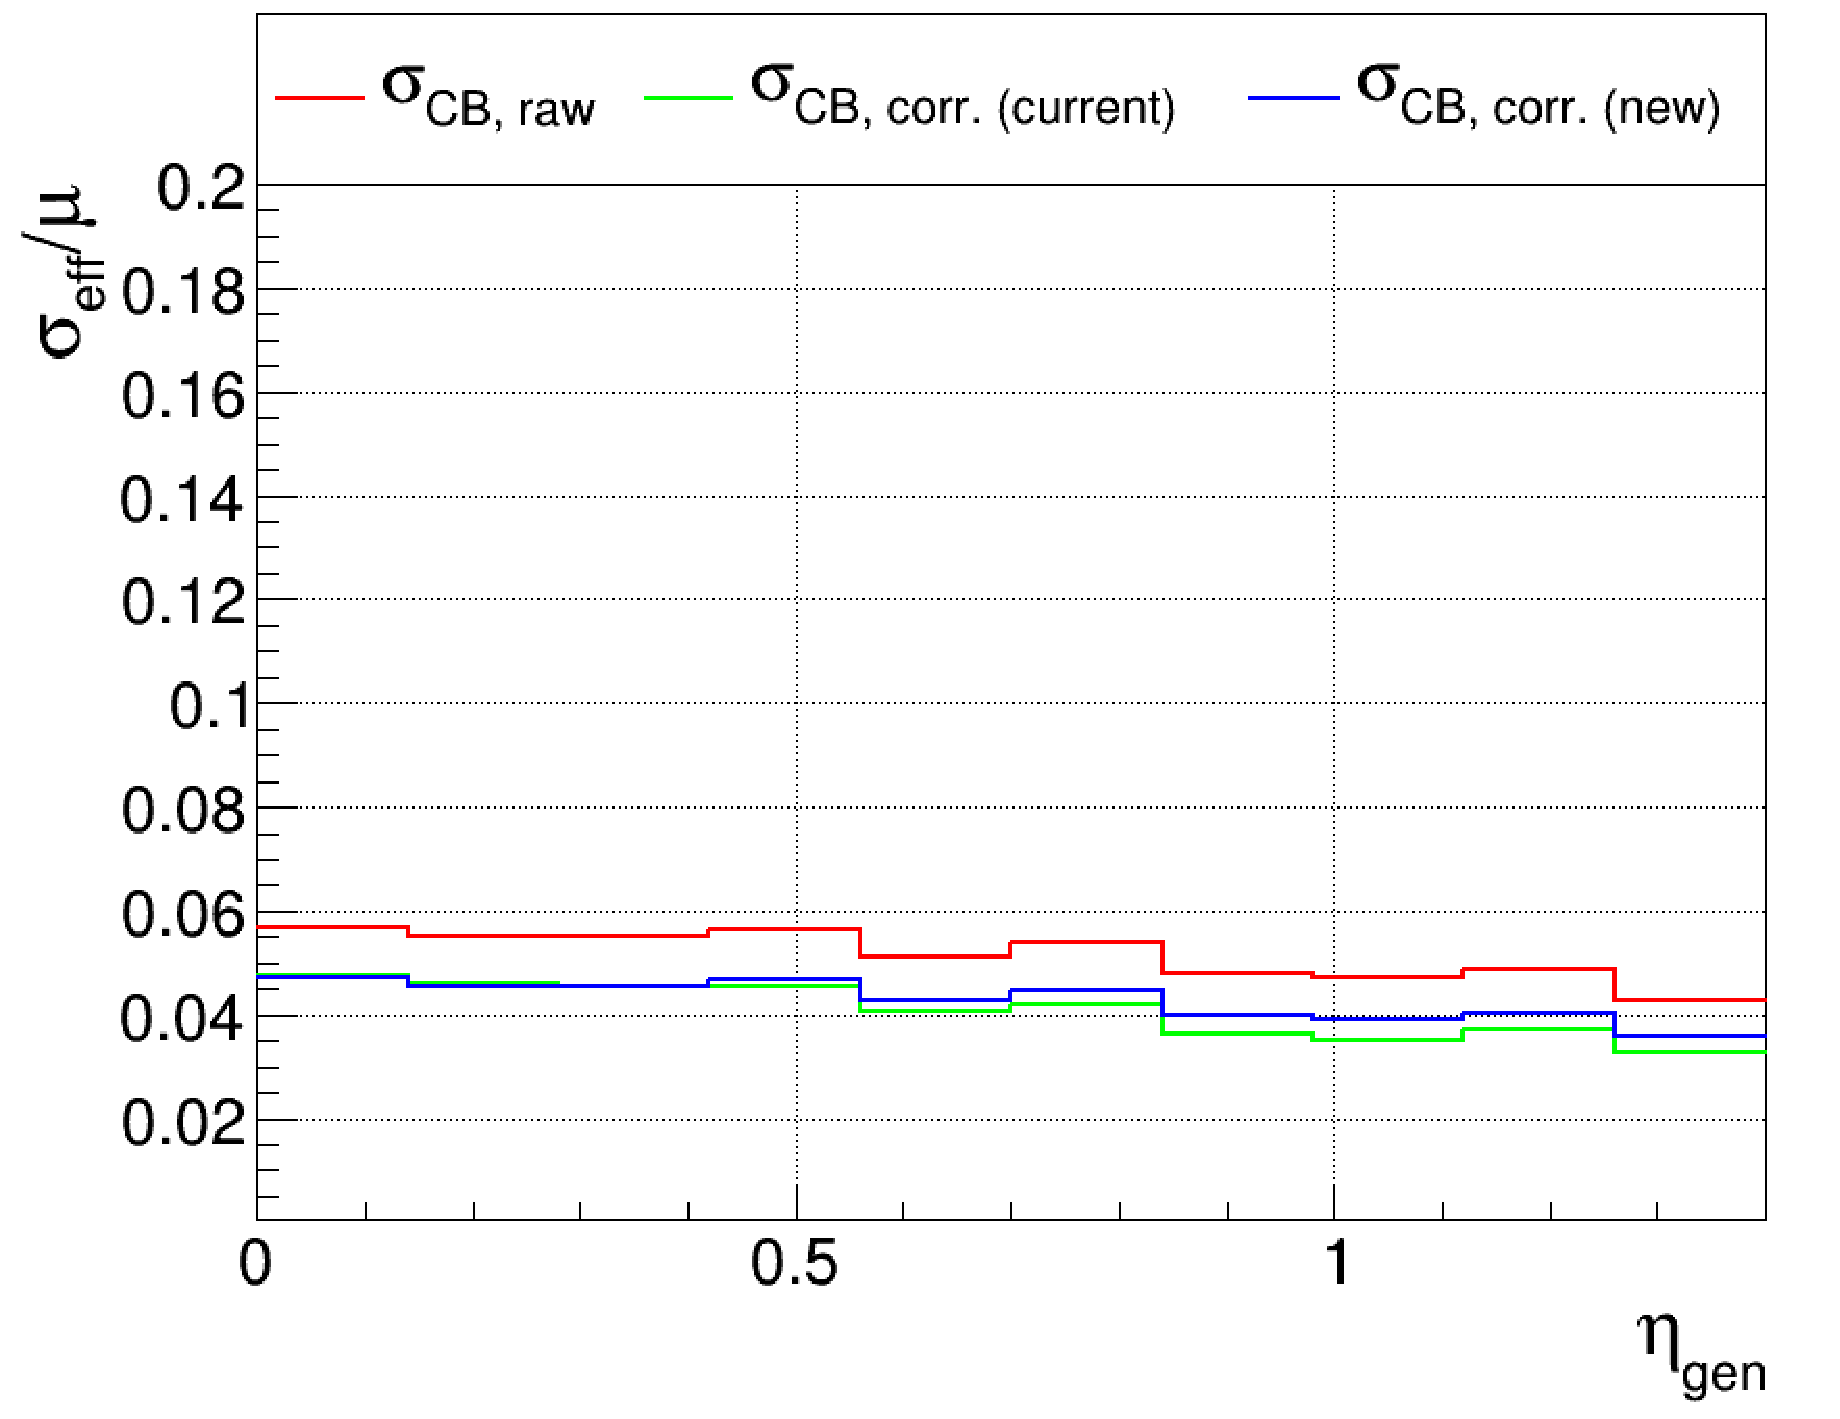
\includegraphics[width=0.495\textwidth]{./plots_pdf/ECAL_plots/plotsPU/EB/FULL/pdf/GENETA/EBFULL_GENETA_0005_0020_EffSigmaOverBins.pdf}
\caption{EB - Full Readout \pt 5--20\GeV.}
\end{figure}


\begin{figure}
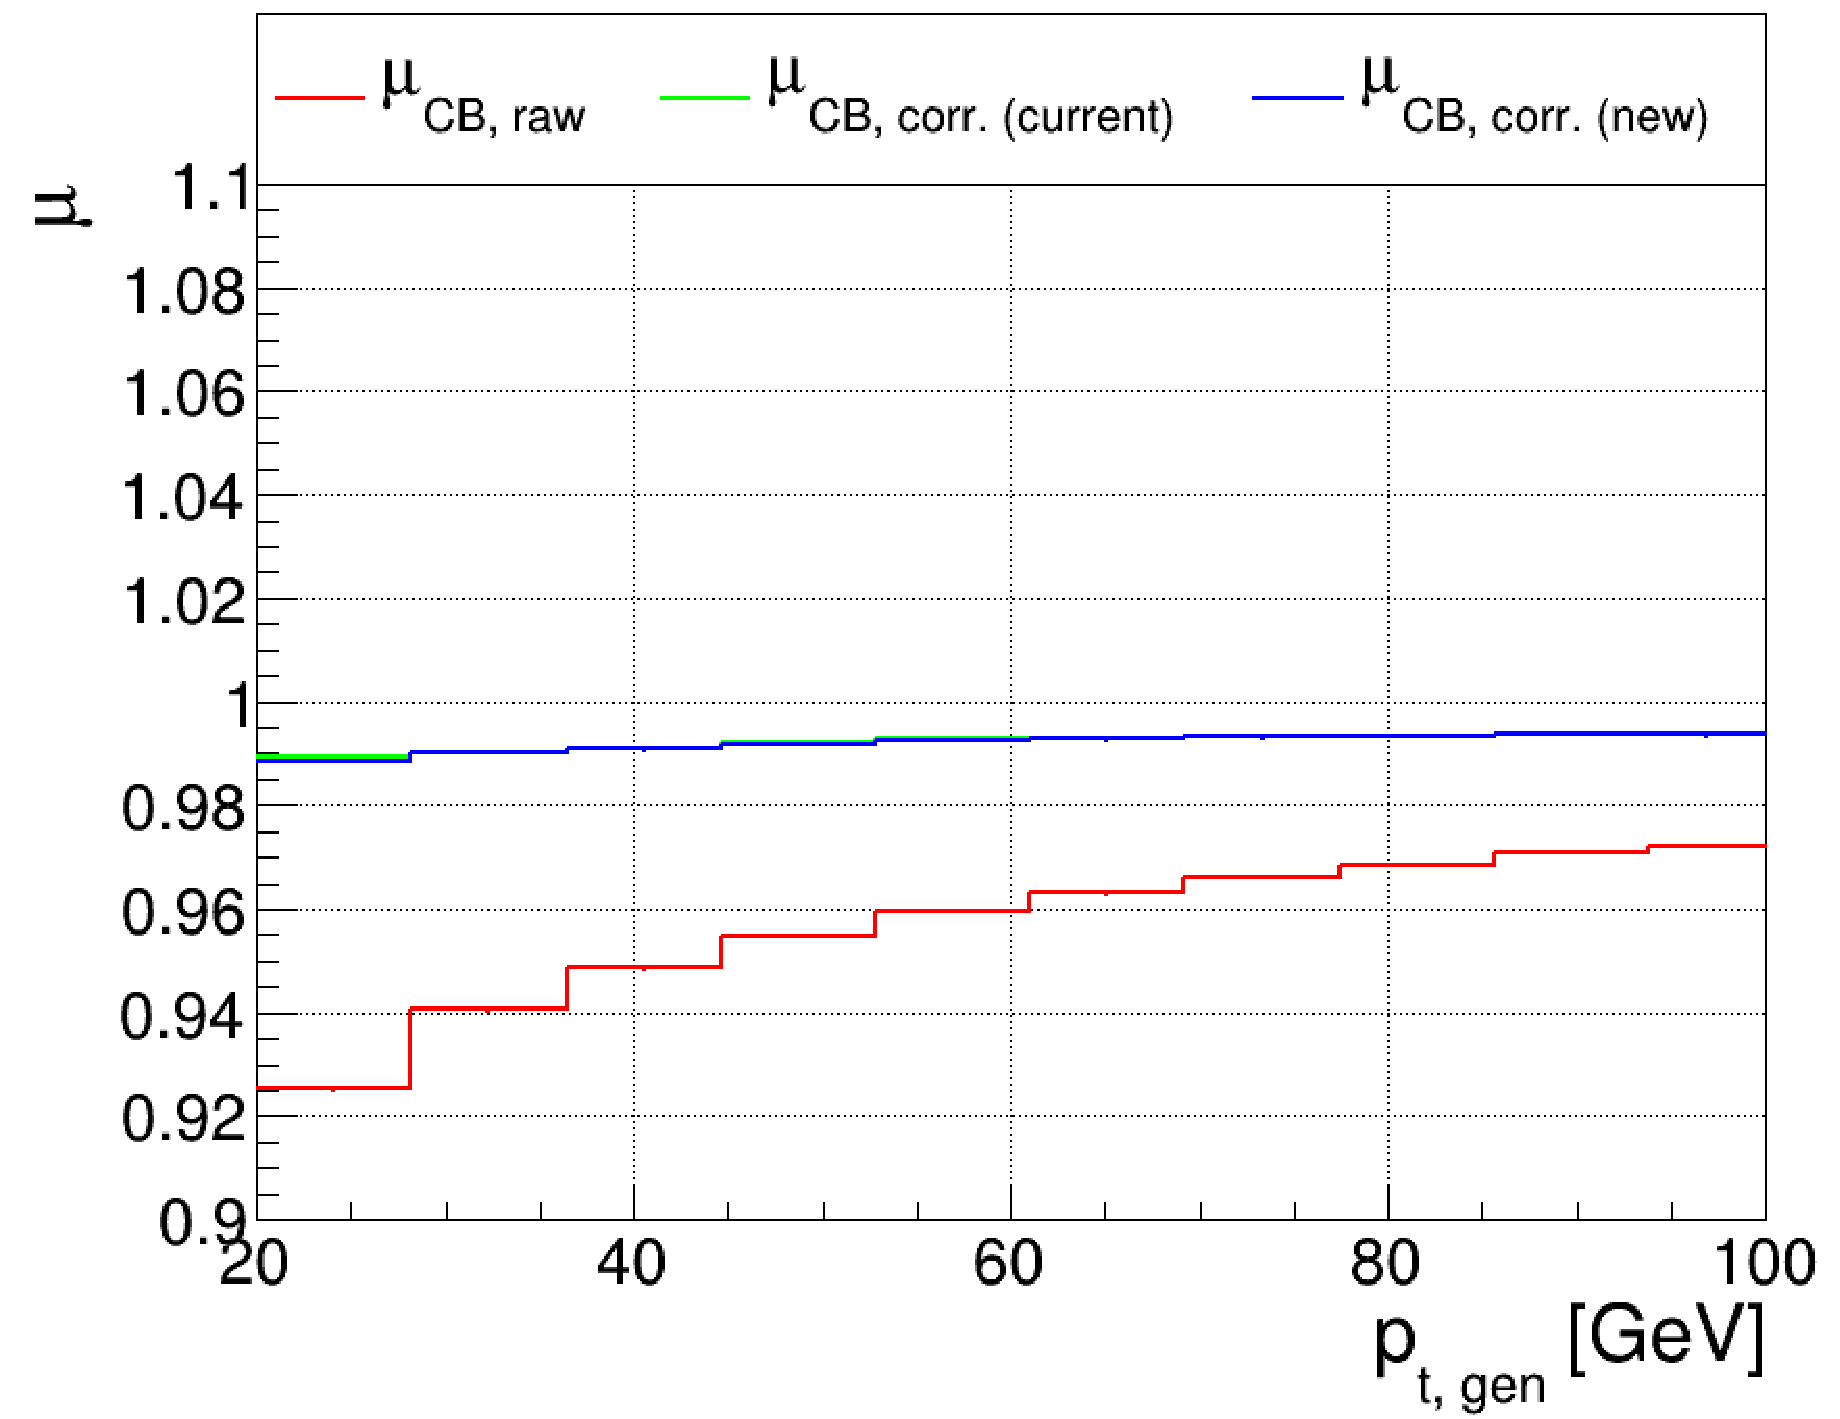
\includegraphics[width=0.495\textwidth]{./plots_pdf/ECAL_plots/plotsPU/EB/FULL/pdf/GENPT/EBFULL_GENPT_0020_0100_MuOverBins.pdf}
\includegraphics[width=0.495\textwidth]{./plots_pdf/ECAL_plots/plotsPU/EB/FULL/pdf/GENPT/EBFULL_GENPT_0020_0100_EffSigmaOverBins.pdf}
%\caption{EB - Full Readout pt 20-100}
%\end{figure}
%\begin{figure}
\includegraphics[width=0.495\textwidth]{./plots_pdf/ECAL_plots/plotsPU/EB/FULL/pdf/GENETA/EBFULL_GENETA_0020_0100_MuOverBins.pdf}
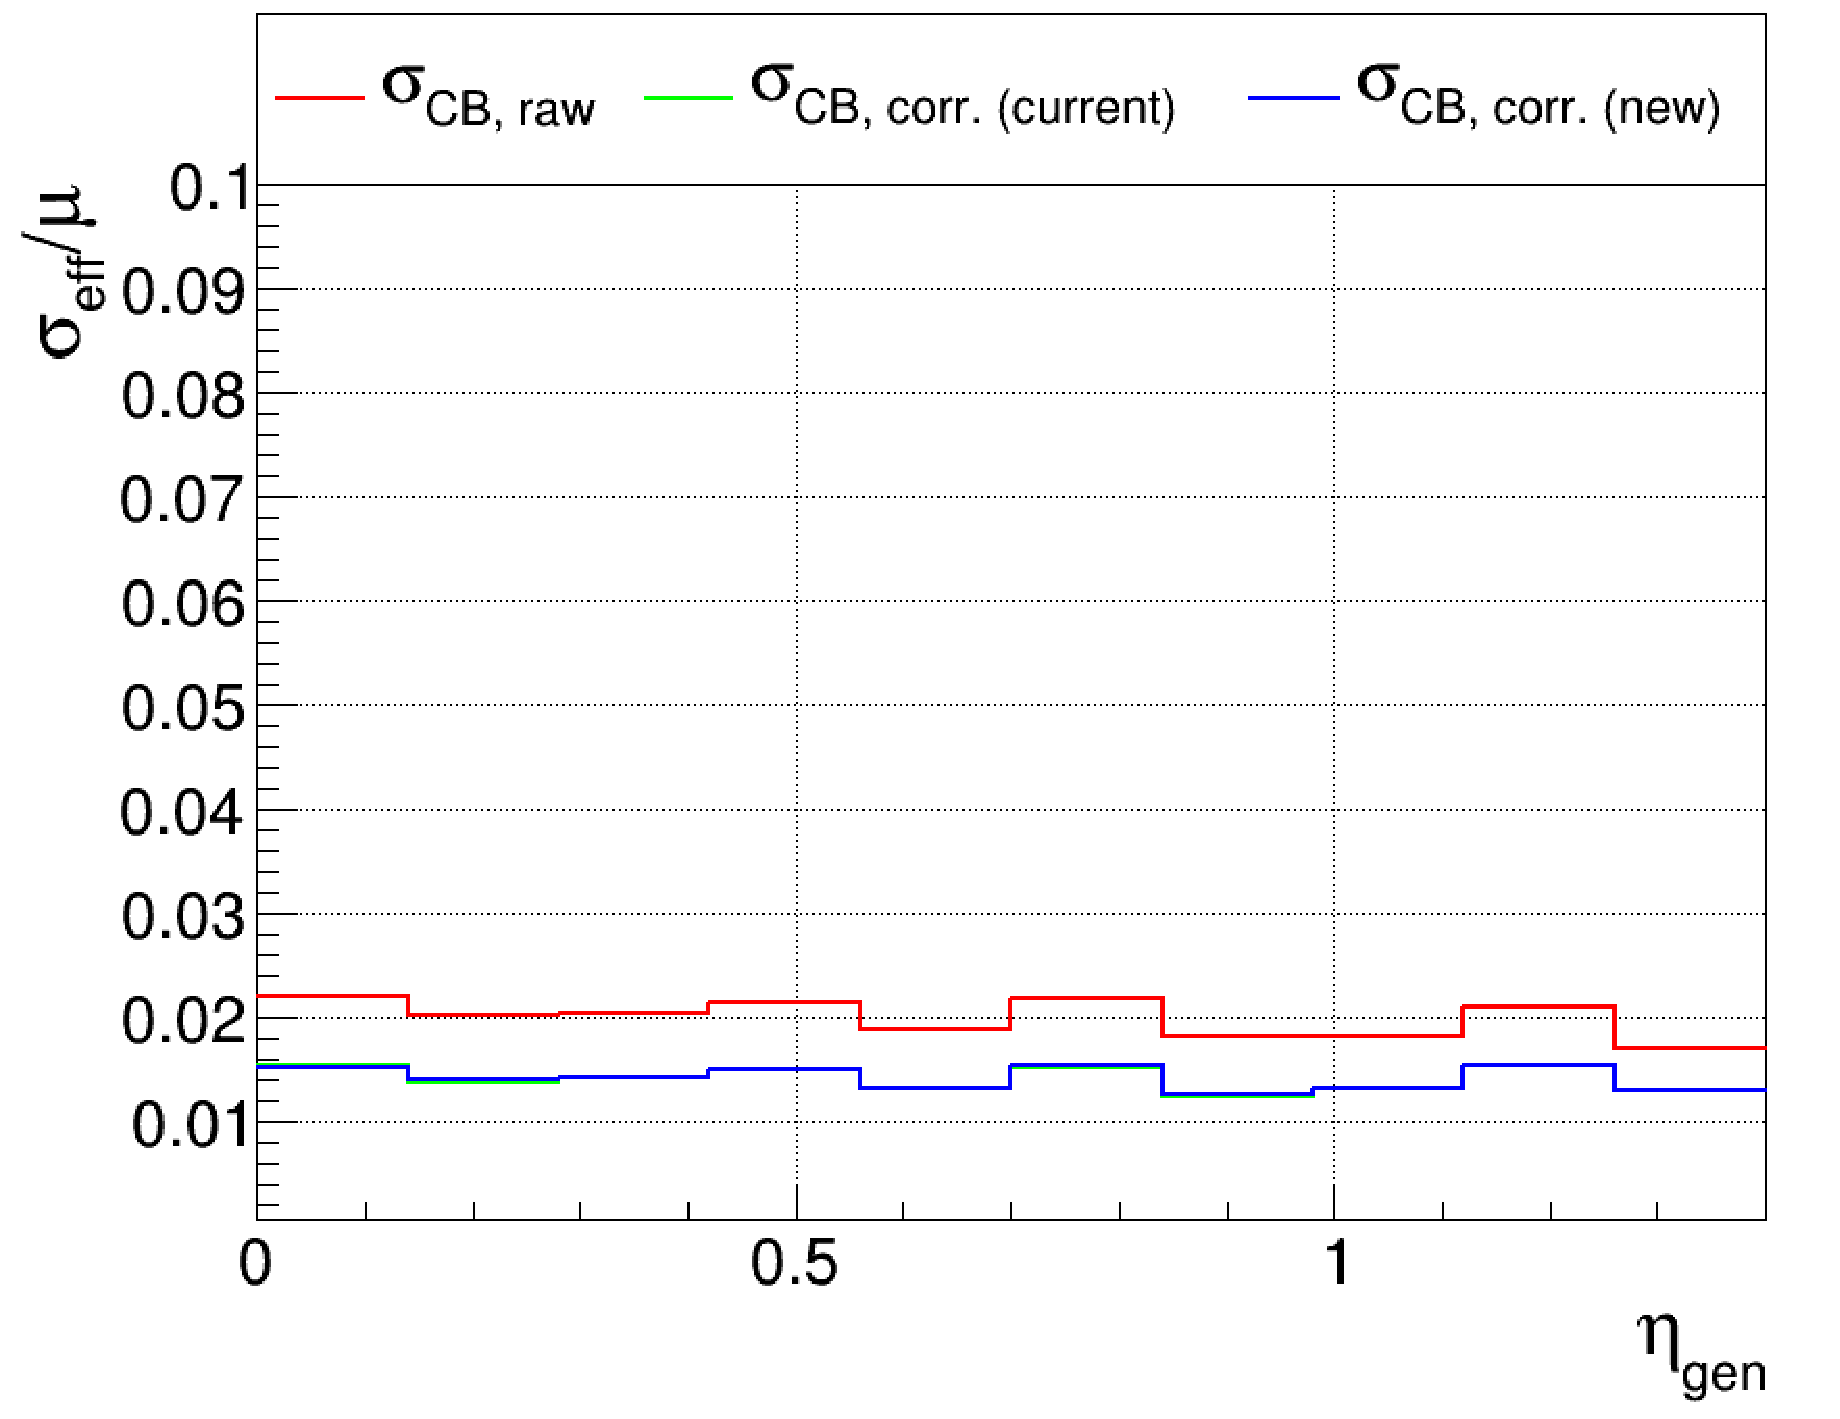
\includegraphics[width=0.495\textwidth]{./plots_pdf/ECAL_plots/plotsPU/EB/FULL/pdf/GENETA/EBFULL_GENETA_0020_0100_EffSigmaOverBins.pdf}
\caption{EB - Full Readout \pt 20--100\GeV.}
\end{figure}

\begin{figure}
\includegraphics[width=0.495\textwidth]{./plots_pdf/ECAL_plots/plotsPU/EB/FULL/pdf/GENPT/EBFULL_GENPT_0100_0300_MuOverBins.pdf}
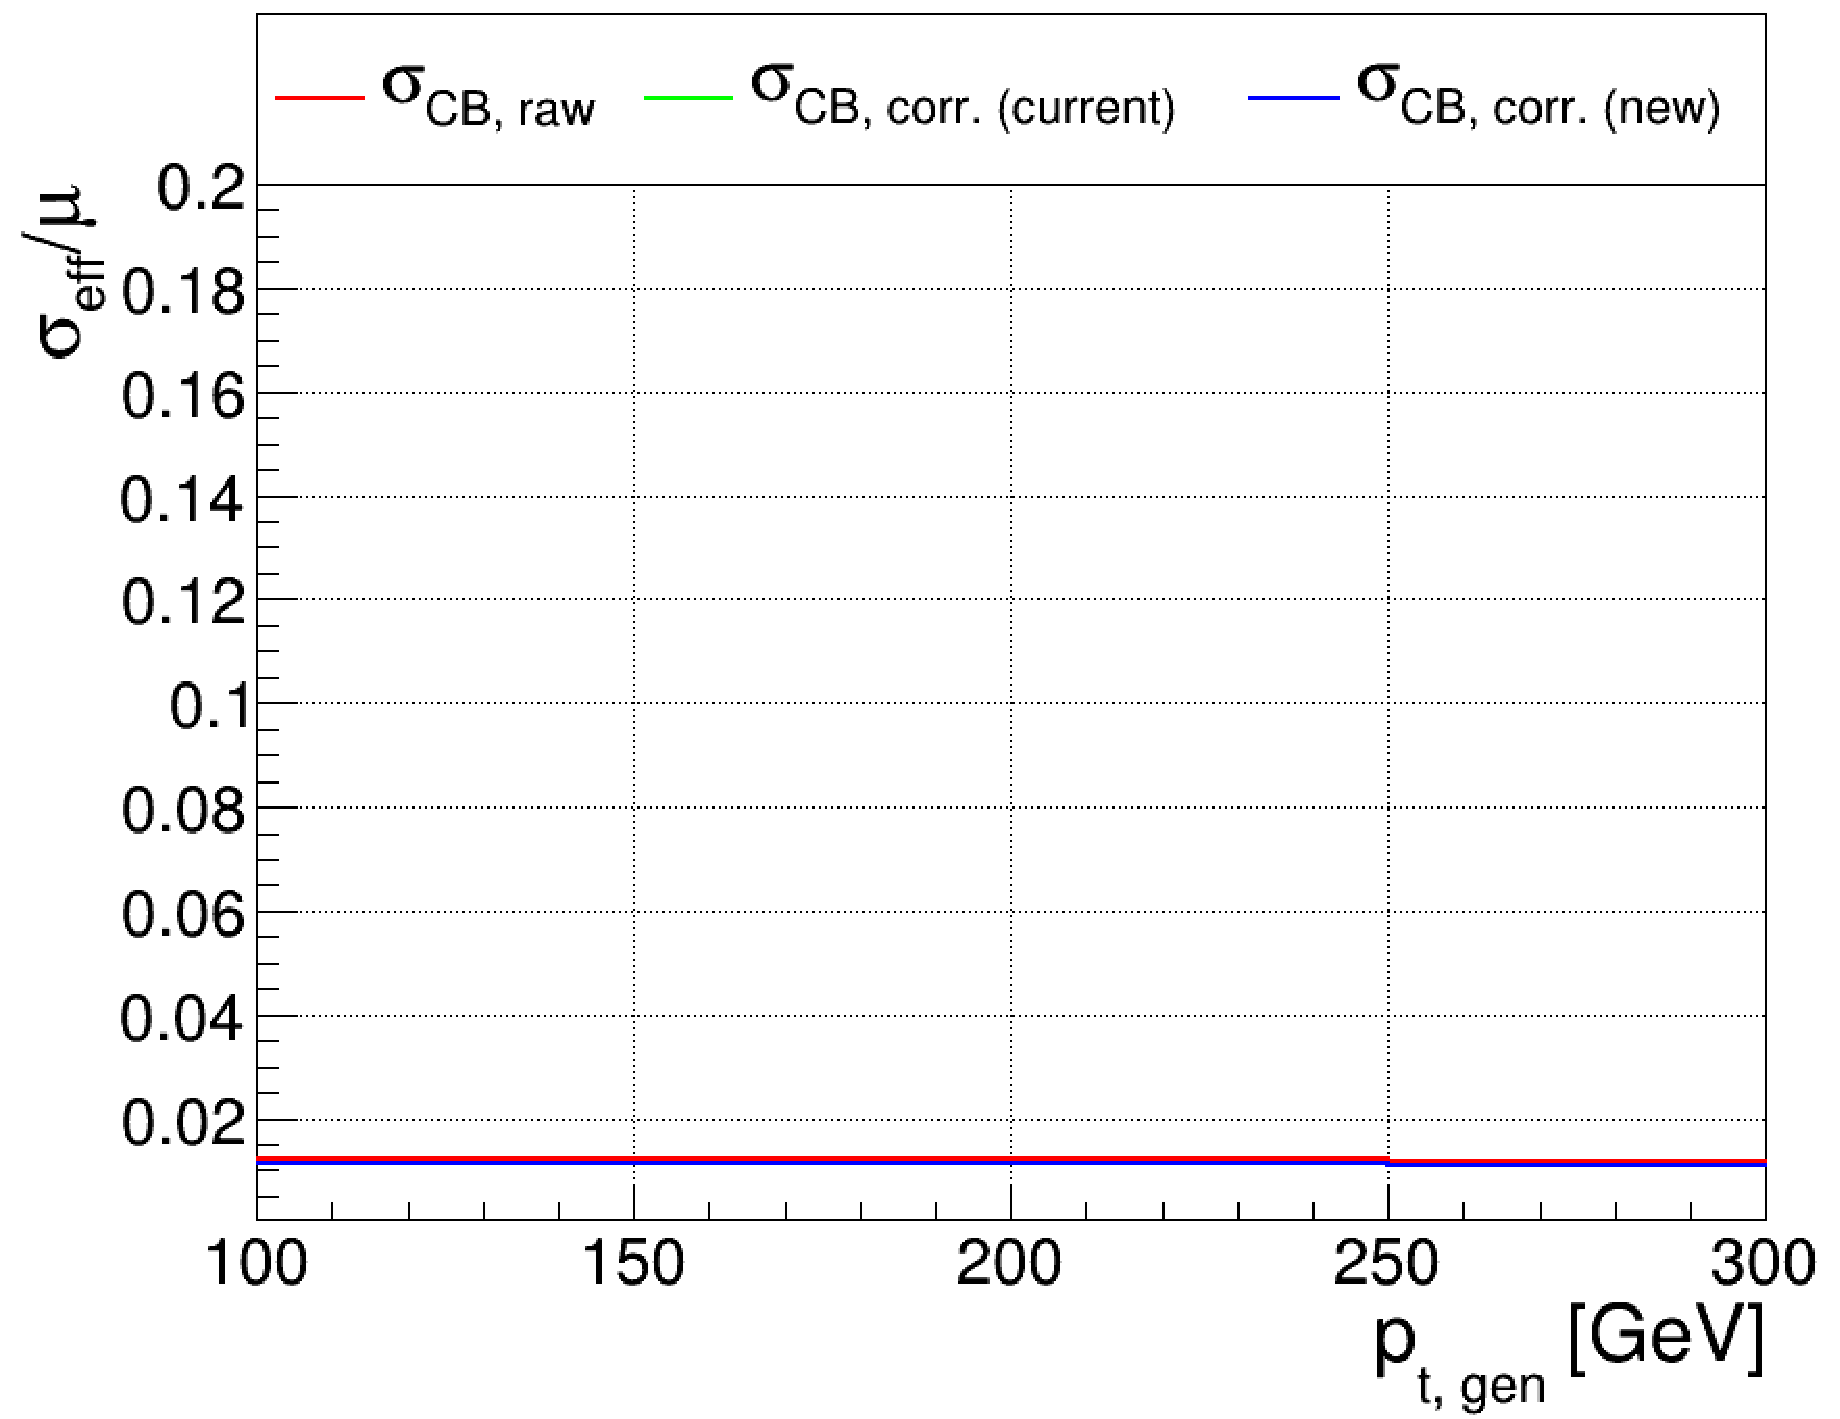
\includegraphics[width=0.495\textwidth]{./plots_pdf/ECAL_plots/plotsPU/EB/FULL/pdf/GENPT/EBFULL_GENPT_0100_0300_EffSigmaOverBins.pdf}
%\caption{EB - Full Readout pt 100-300}
%\end{figure}
%\begin{figure}
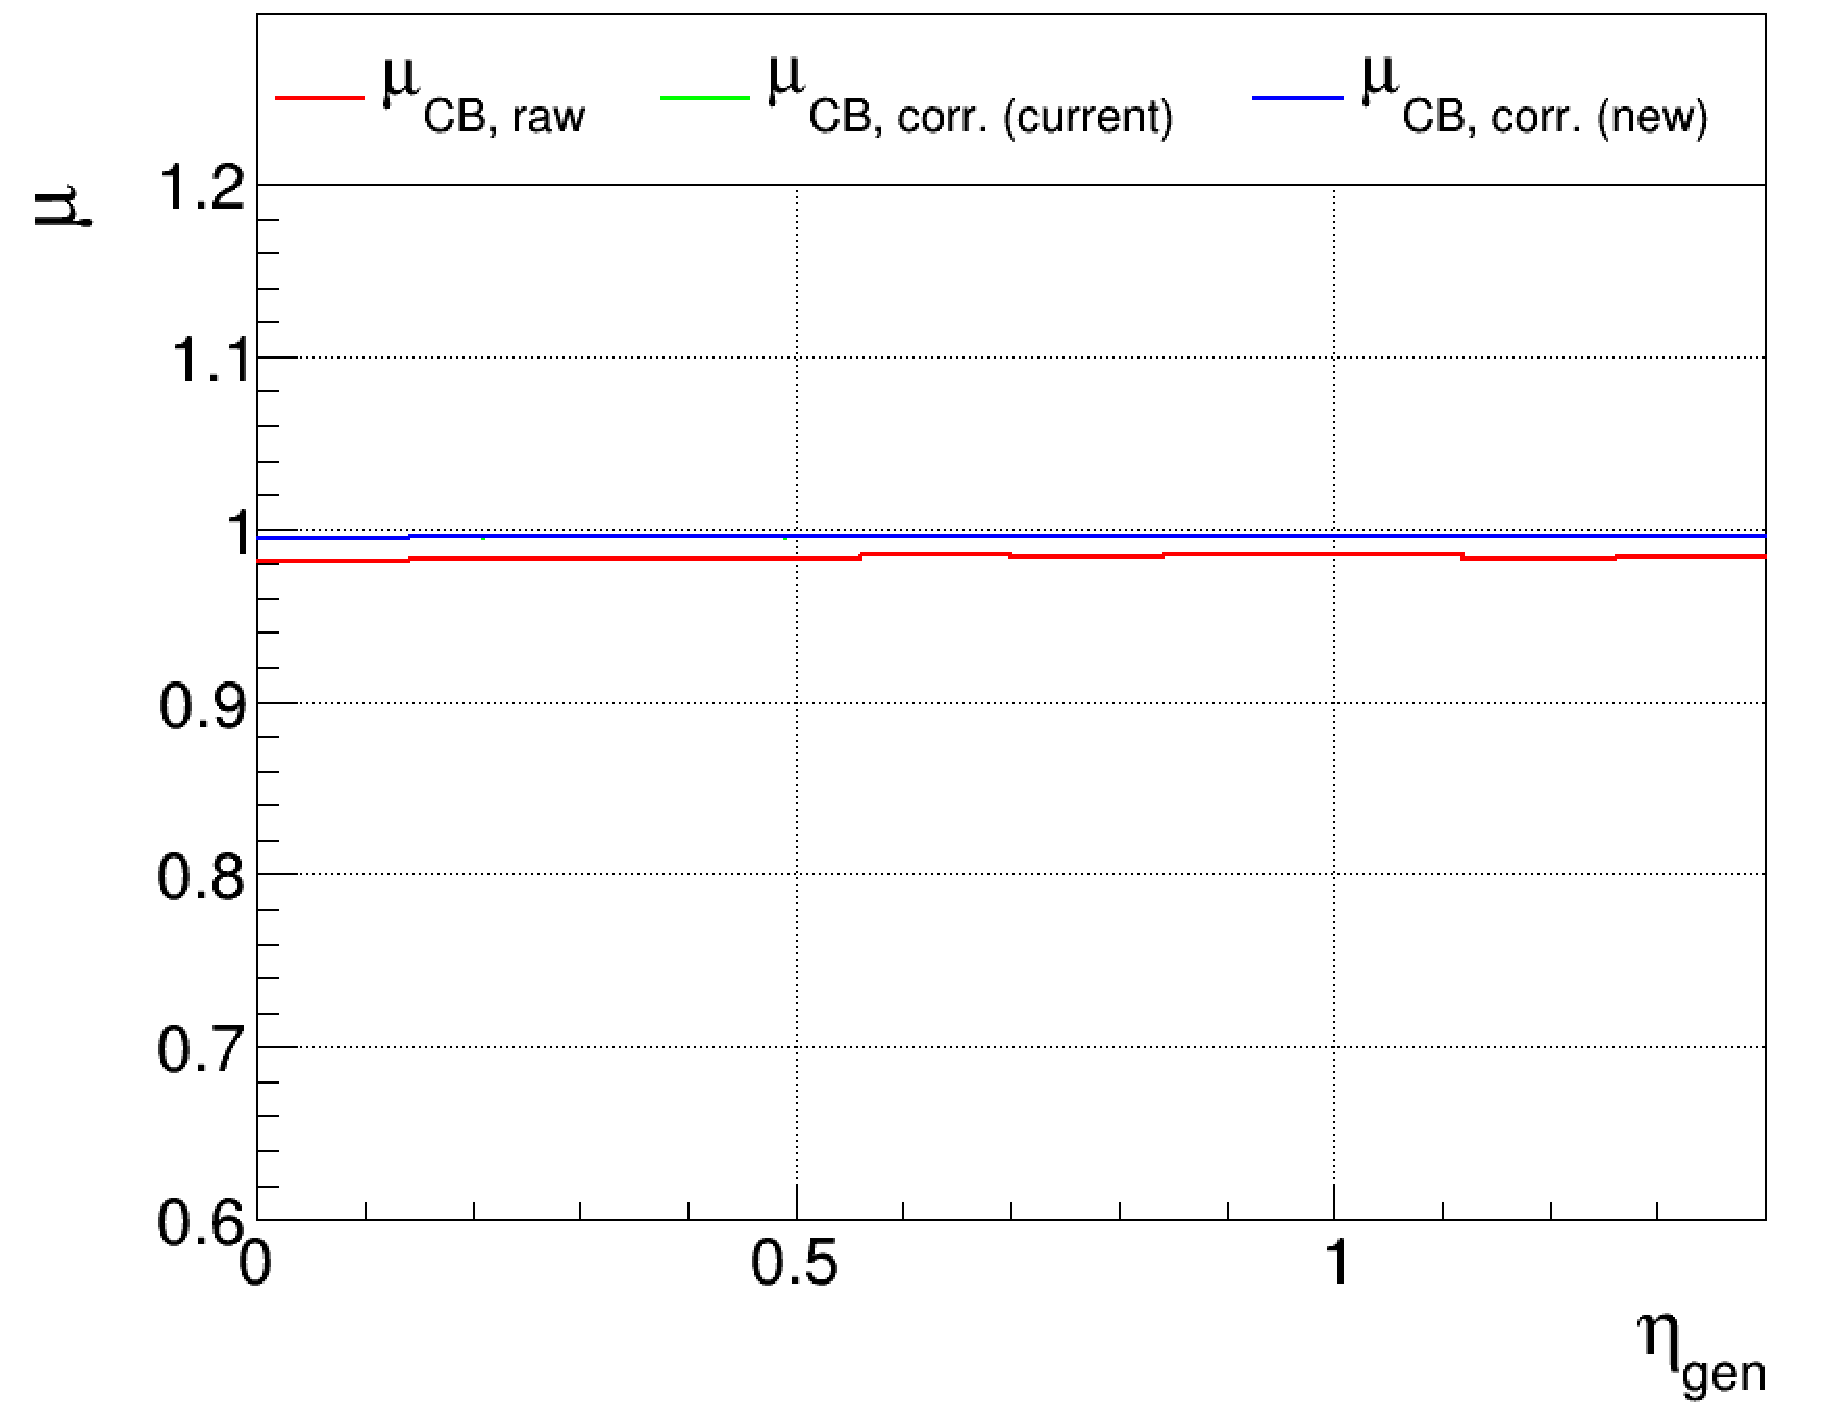
\includegraphics[width=0.495\textwidth]{./plots_pdf/ECAL_plots/plotsPU/EB/FULL/pdf/GENETA/EBFULL_GENETA_0100_0300_MuOverBins.pdf}
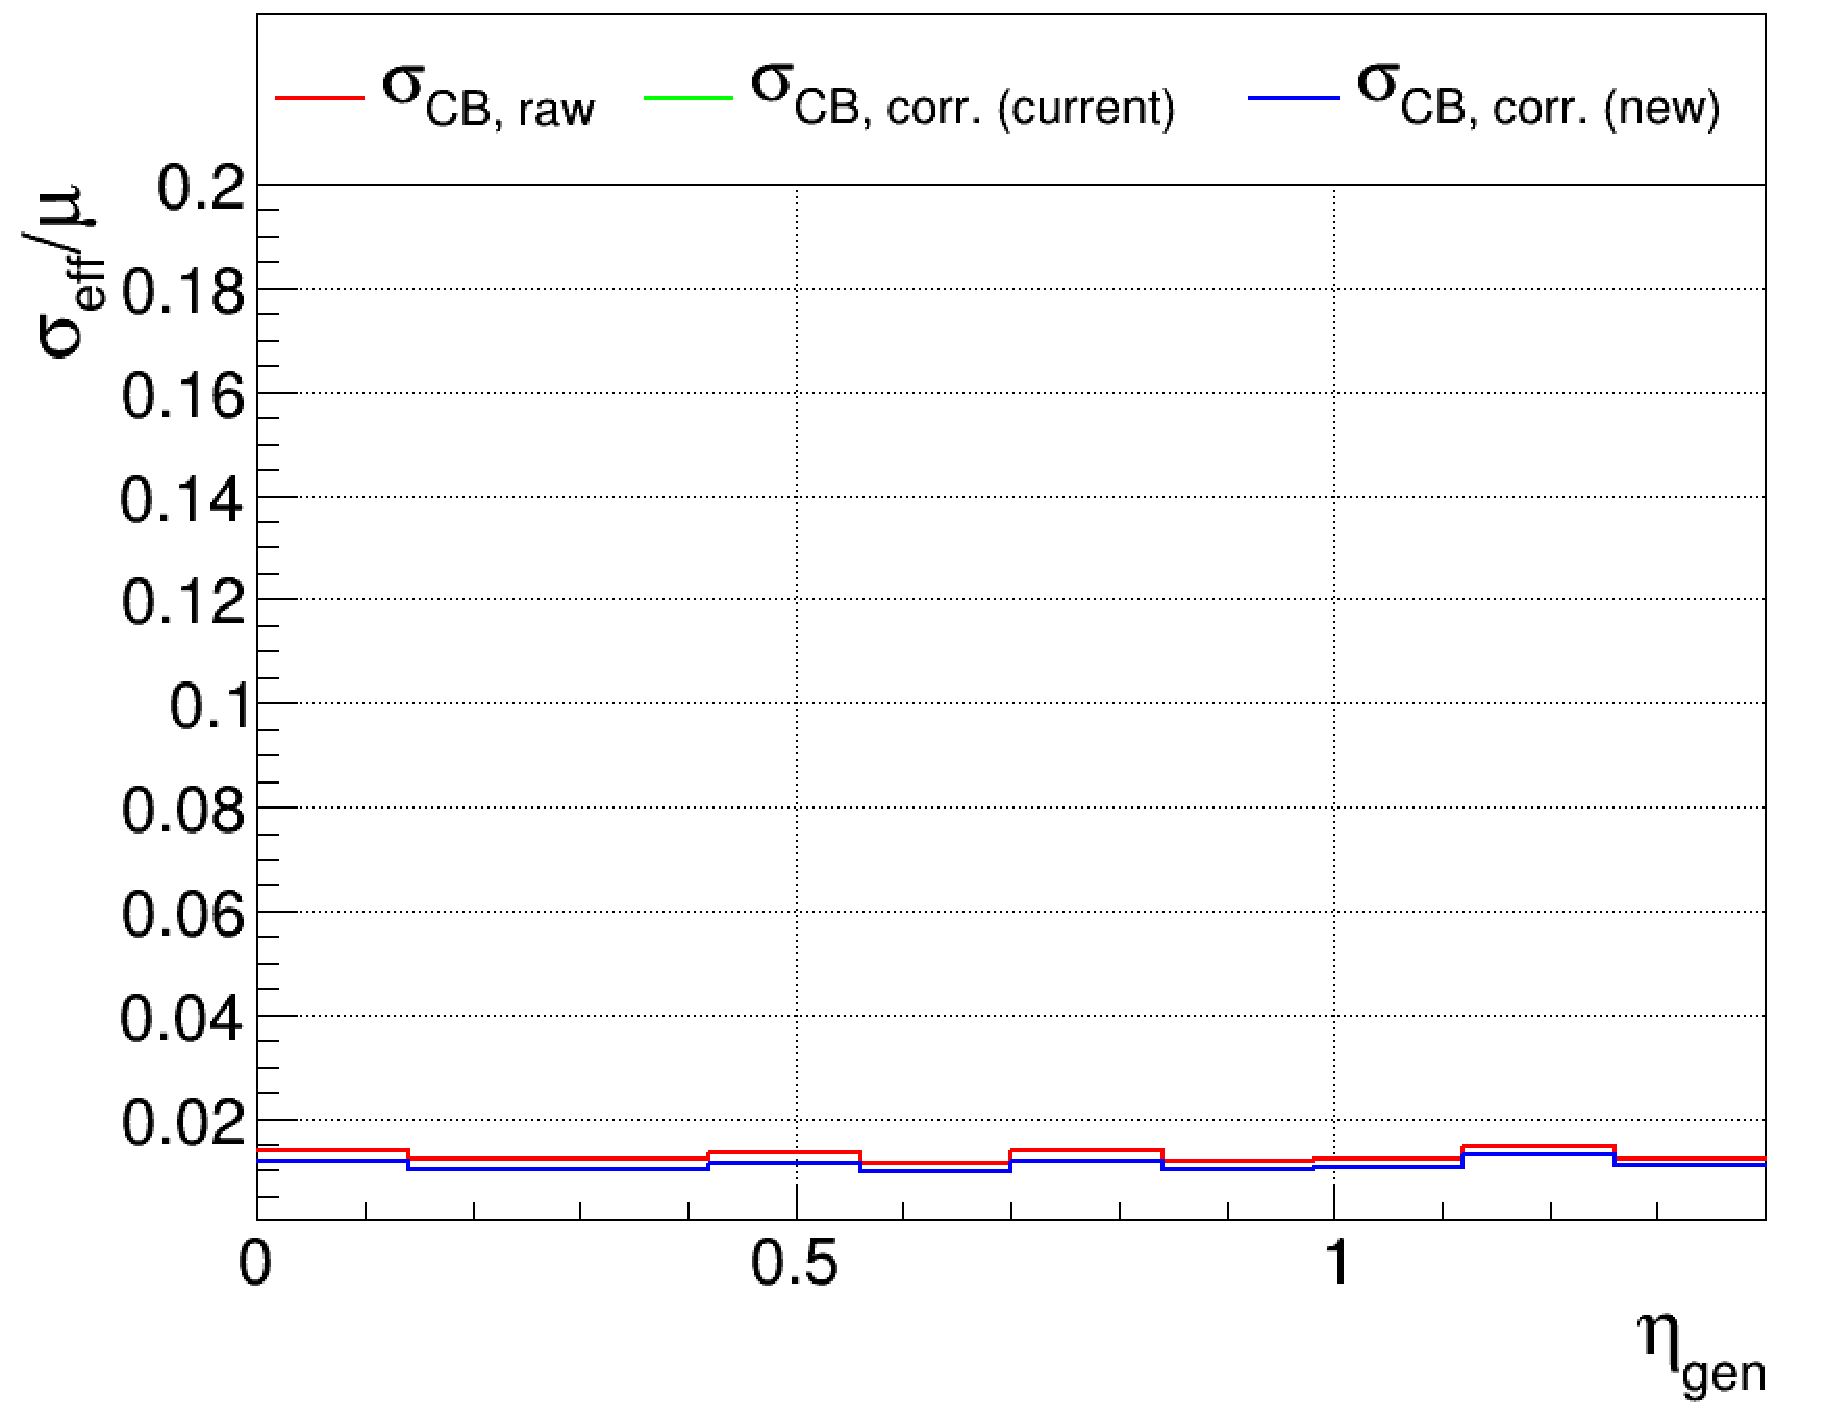
\includegraphics[width=0.495\textwidth]{./plots_pdf/ECAL_plots/plotsPU/EB/FULL/pdf/GENETA/EBFULL_GENETA_0100_0300_EffSigmaOverBins.pdf}
\caption{EB - Full Readout \pt 100-300\GeV}
\end{figure}





\begin{figure}
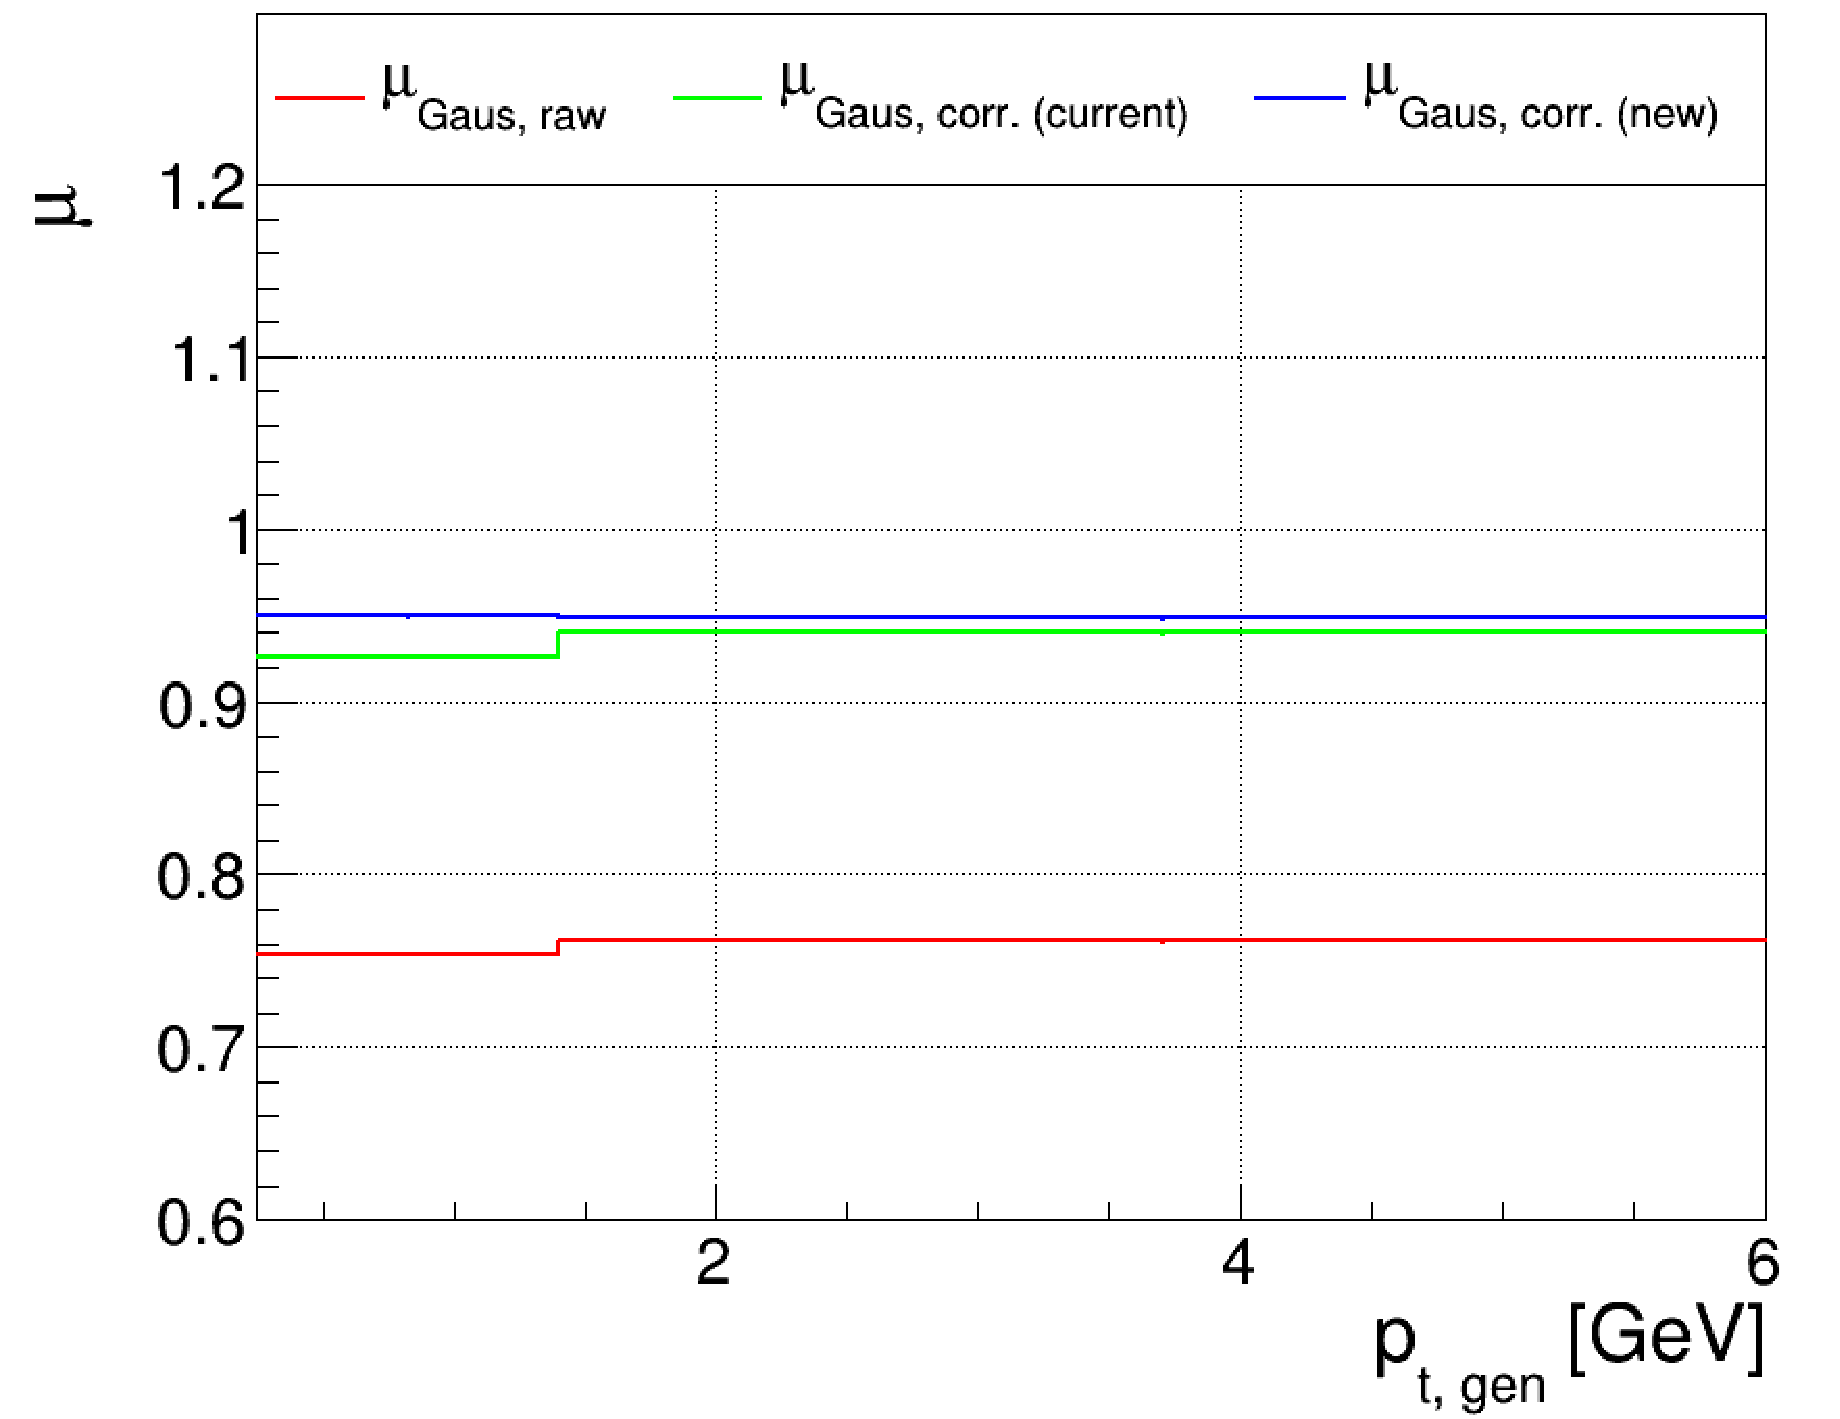
\includegraphics[width=0.495\textwidth]{./plots_pdf/ECAL_plots/plotsPU/EB/ZS/pdf/GENPT/EBZS_GENPT_0000_0006_MuOverBins.pdf}
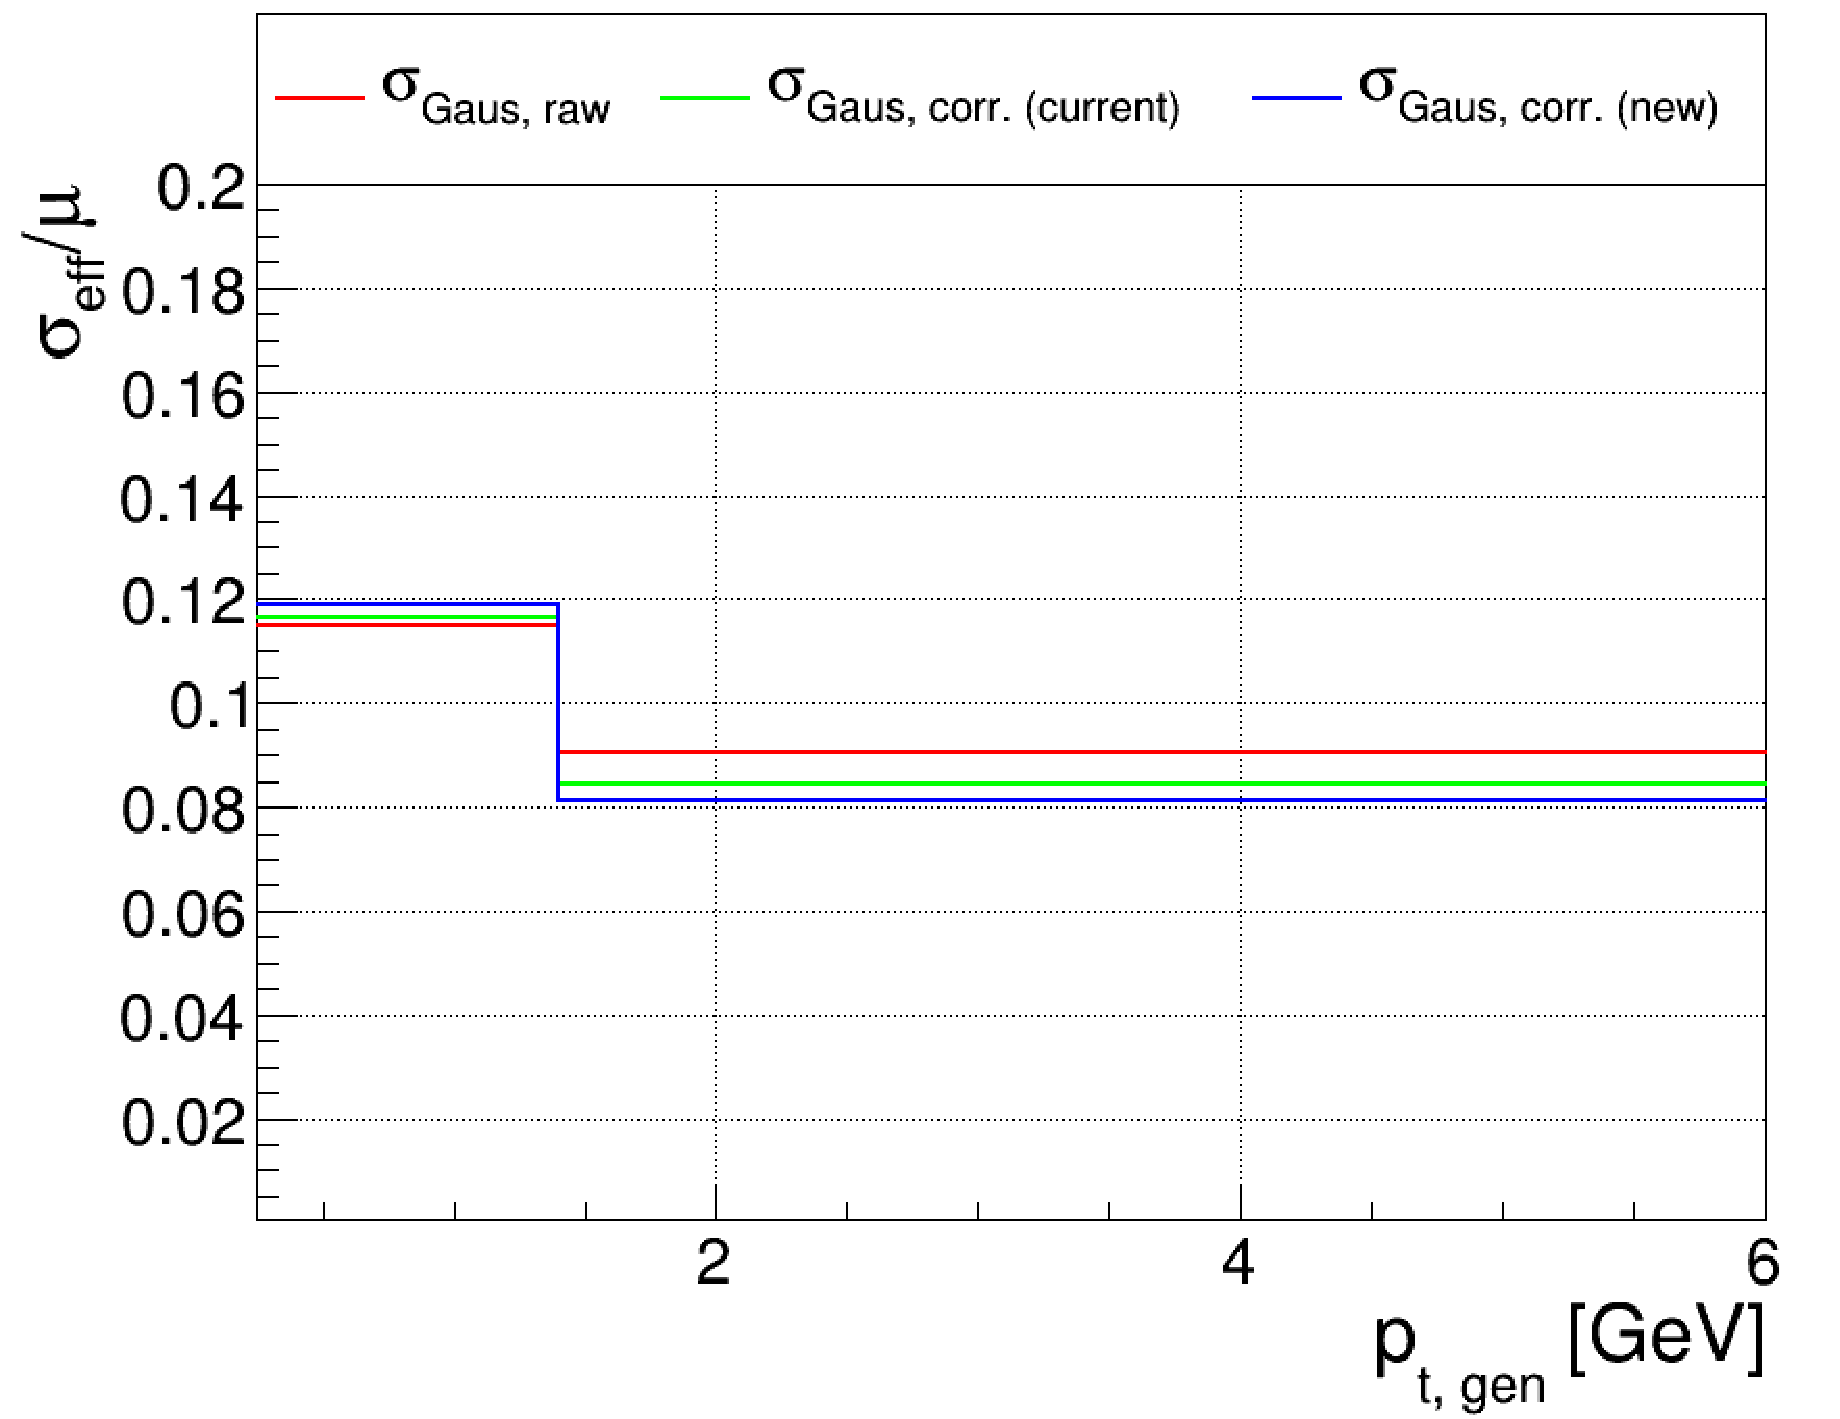
\includegraphics[width=0.495\textwidth]{./plots_pdf/ECAL_plots/plotsPU/EB/ZS/pdf/GENPT/EBZS_GENPT_0000_0006_EffSigmaOverBins.pdf}

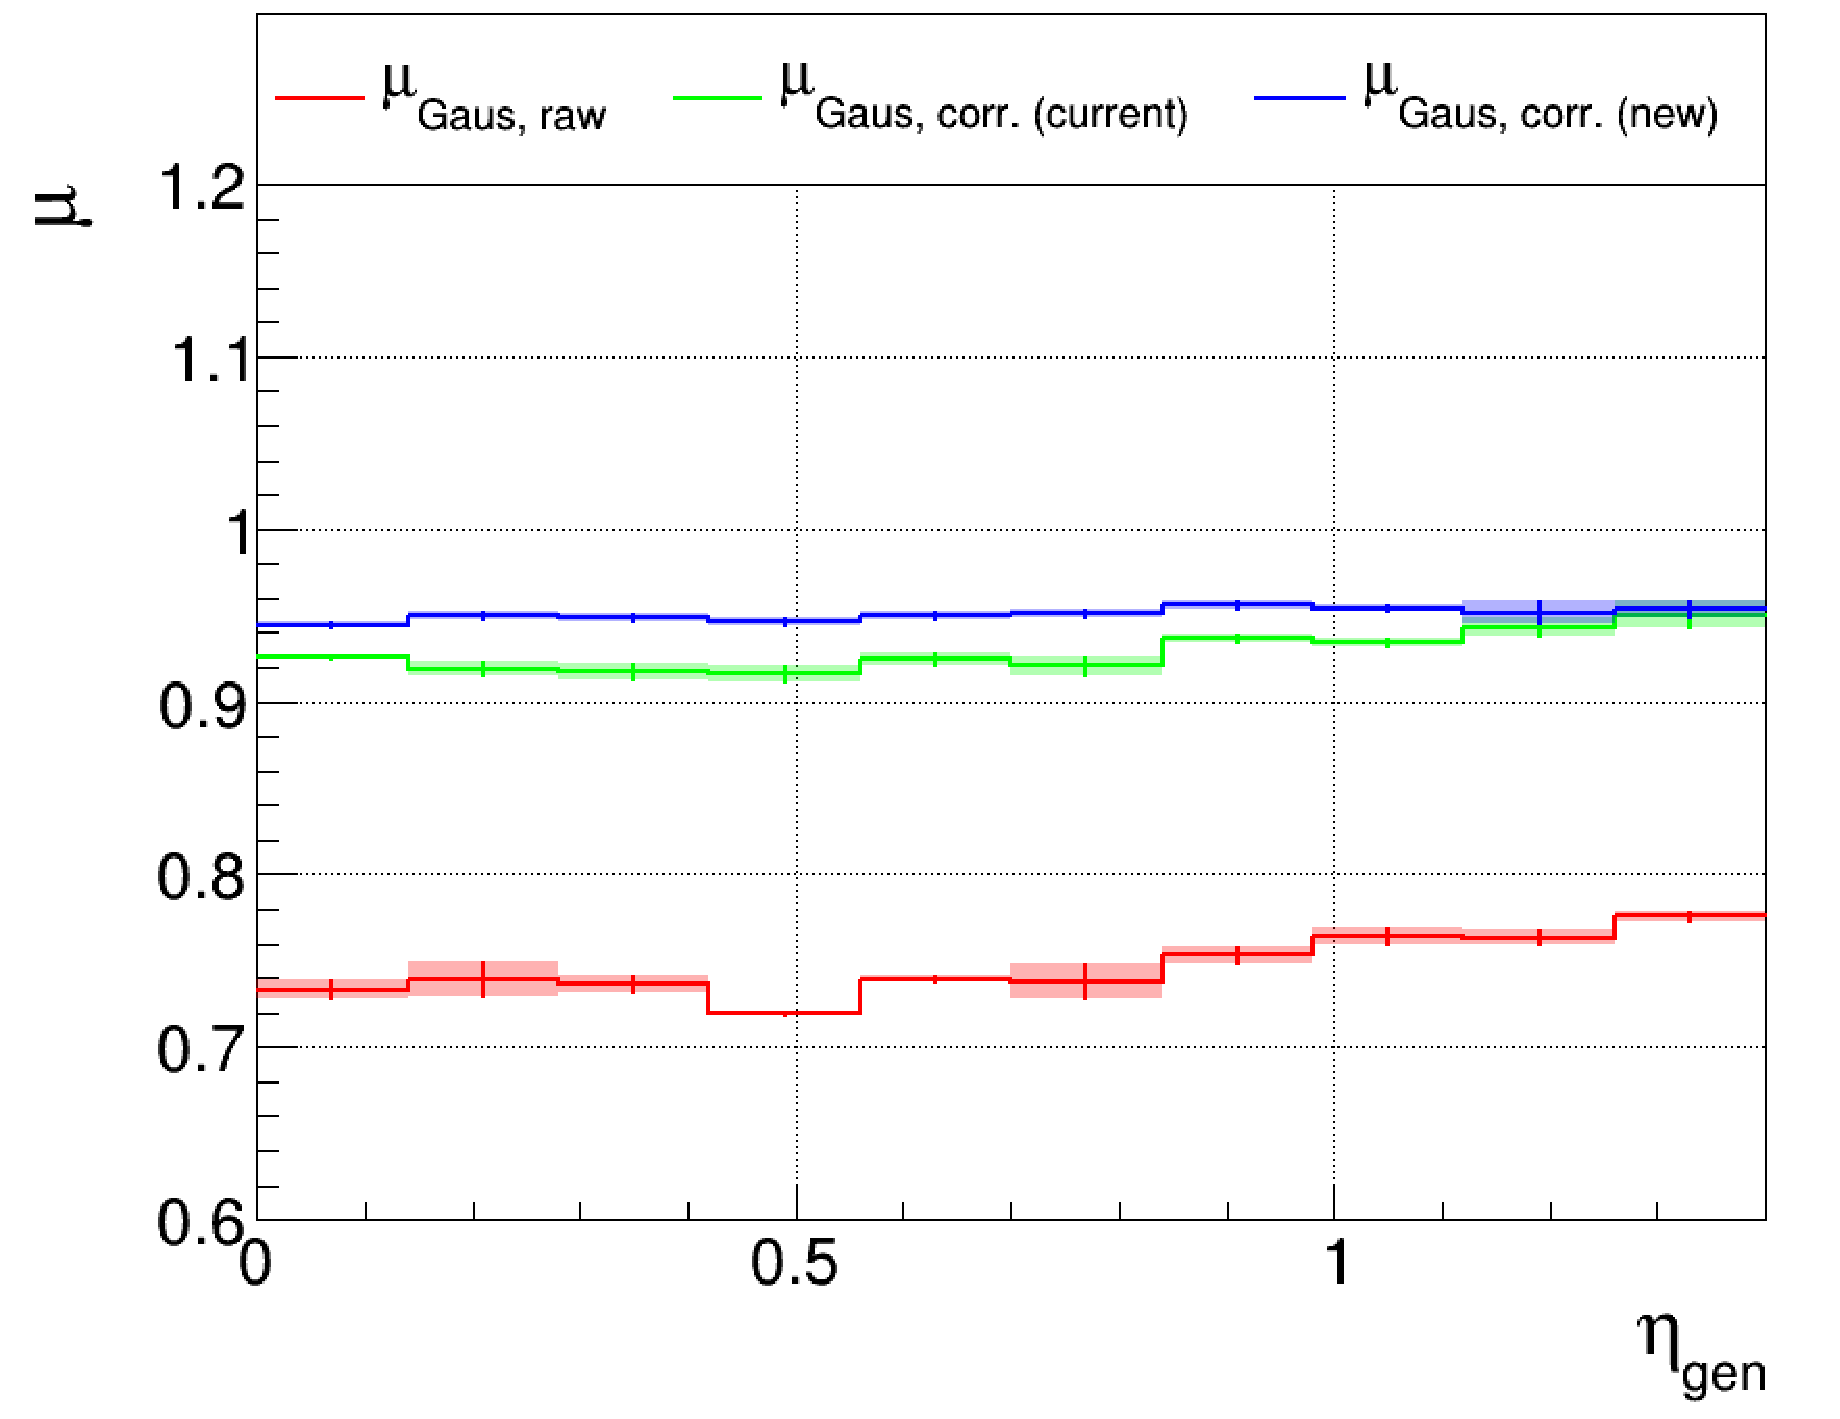
\includegraphics[width=0.495\textwidth]{./plots_pdf/ECAL_plots/plotsPU/EB/ZS/pdf/GENETA/EBZS_GENETA_0000_0006_MuOverBins.pdf}
\includegraphics[width=0.495\textwidth]{./plots_pdf/ECAL_plots/plotsPU/EB/ZS/pdf/GENETA/EBZS_GENETA_0000_0006_EffSigmaOverBins.pdf}
\caption[$\mu$ ($\sigma_\mathrm{eff}$) vs \pt of PF ECAL cluster - EB ZS readout PU  senario]{Mean response (resolution) defined by Raw PF ECAL clusters (red), the calibration derived earlier in Ru\
n3 based on 126X (green), and the new correction from 2024 simulation sample based on 133X (blue). \pt 0--6\GeV PU EB ZS readout PU senario.}
\label{fig:PU_EBZS}
\end{figure}

%% %\begin{figure}
%% \includegraphics[width=0.495\textwidth]{./plots_pdf/ECAL_plots/plotsPU/EB/ZS/pdf/GENPT/EBZS_GENPT_0006_0025_MuOverBins.pdf}
%% 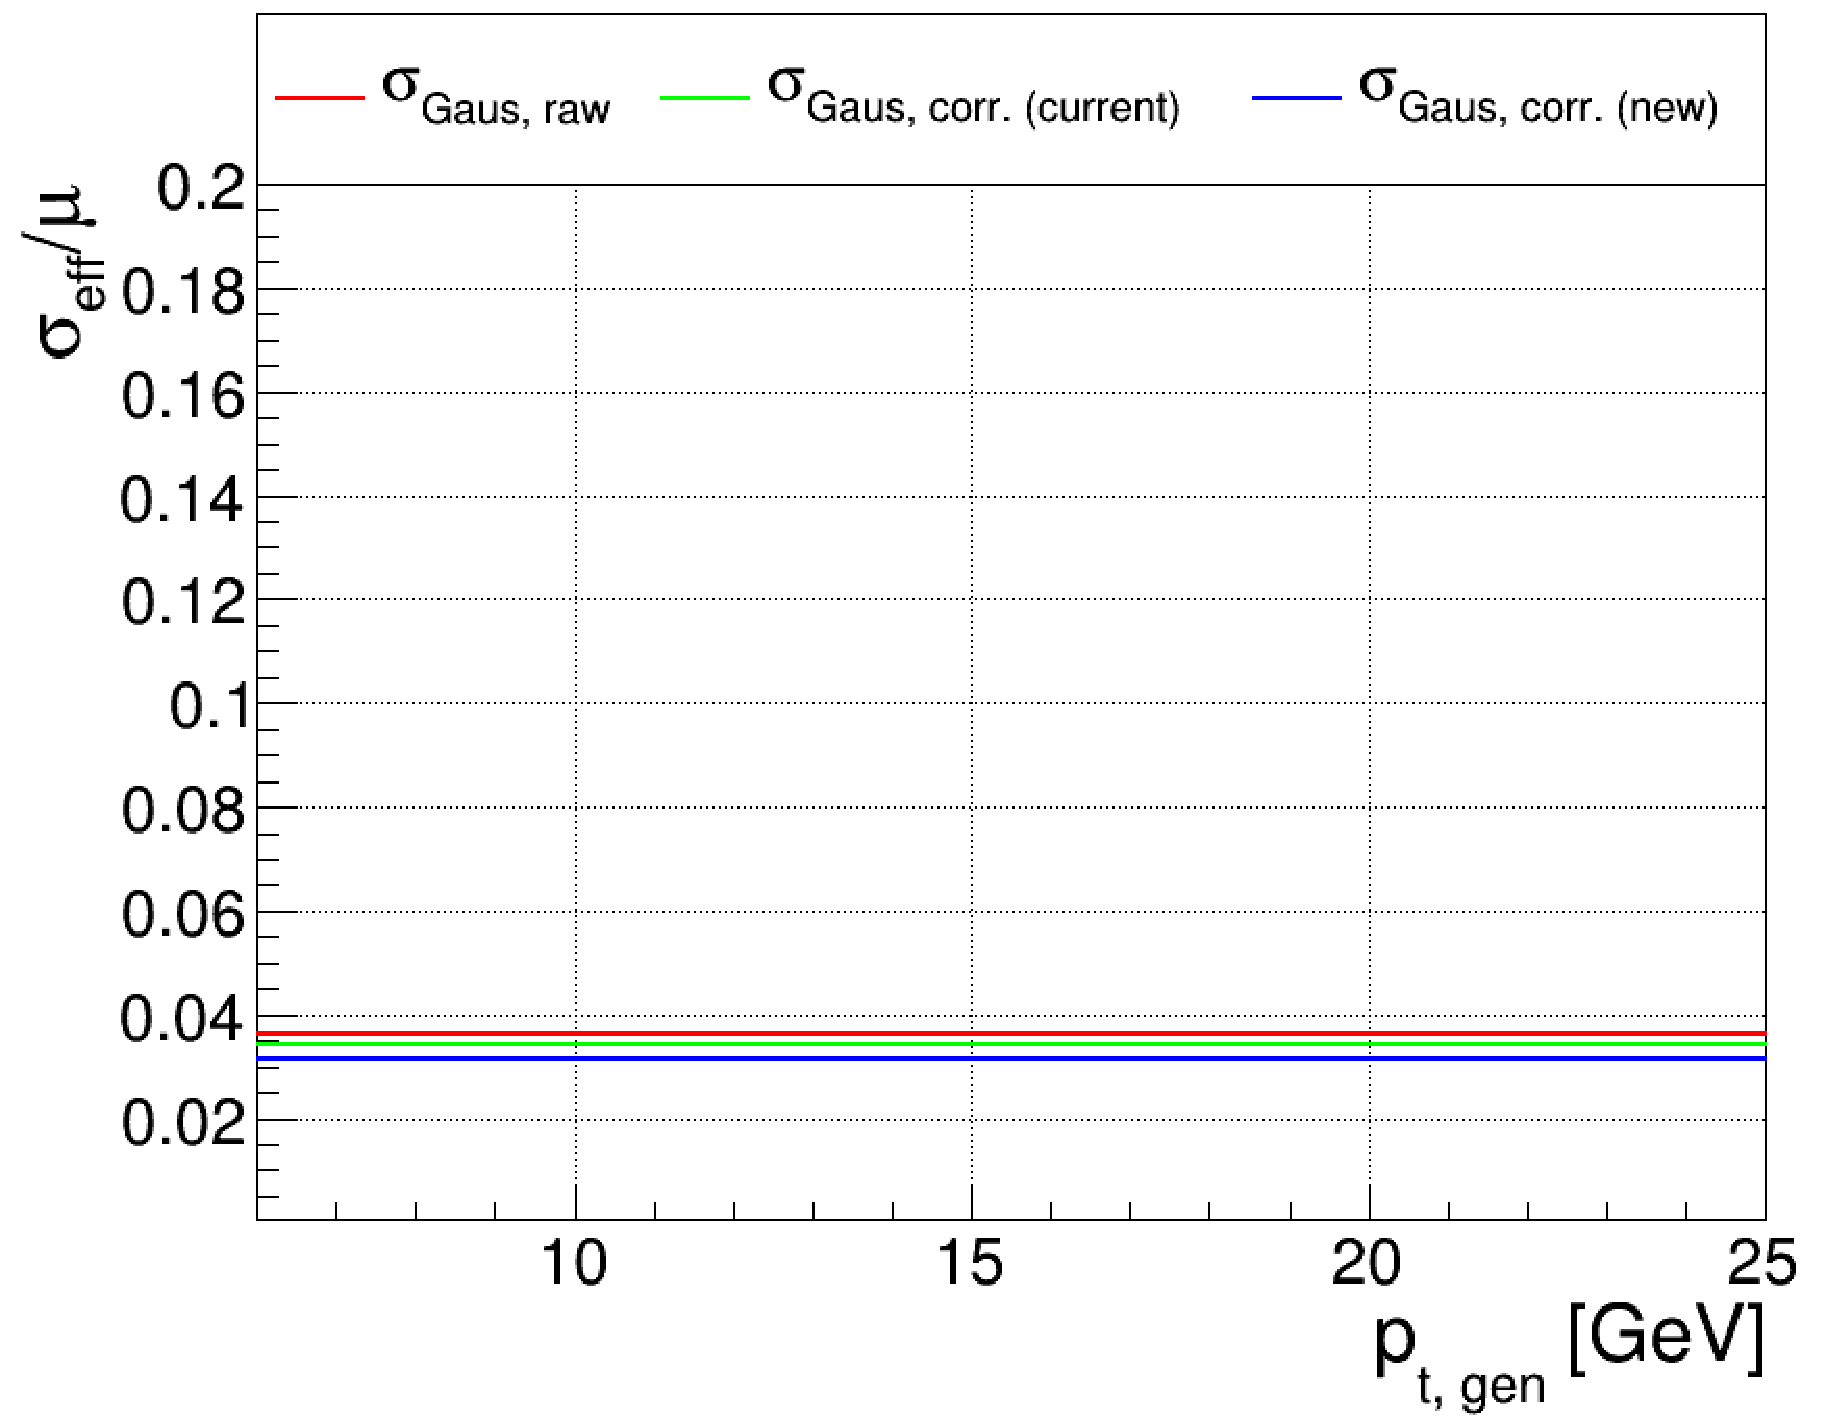
\includegraphics[width=0.495\textwidth]{./plots_pdf/ECAL_plots/plotsPU/EB/ZS/pdf/GENPT/EBZS_GENPT_0006_0025_EffSigmaOverBins.pdf}
%% %\caption{EB - ZS Readout pt 6-25}
%% %\end{figure}
%% %\begin{figure}
%% 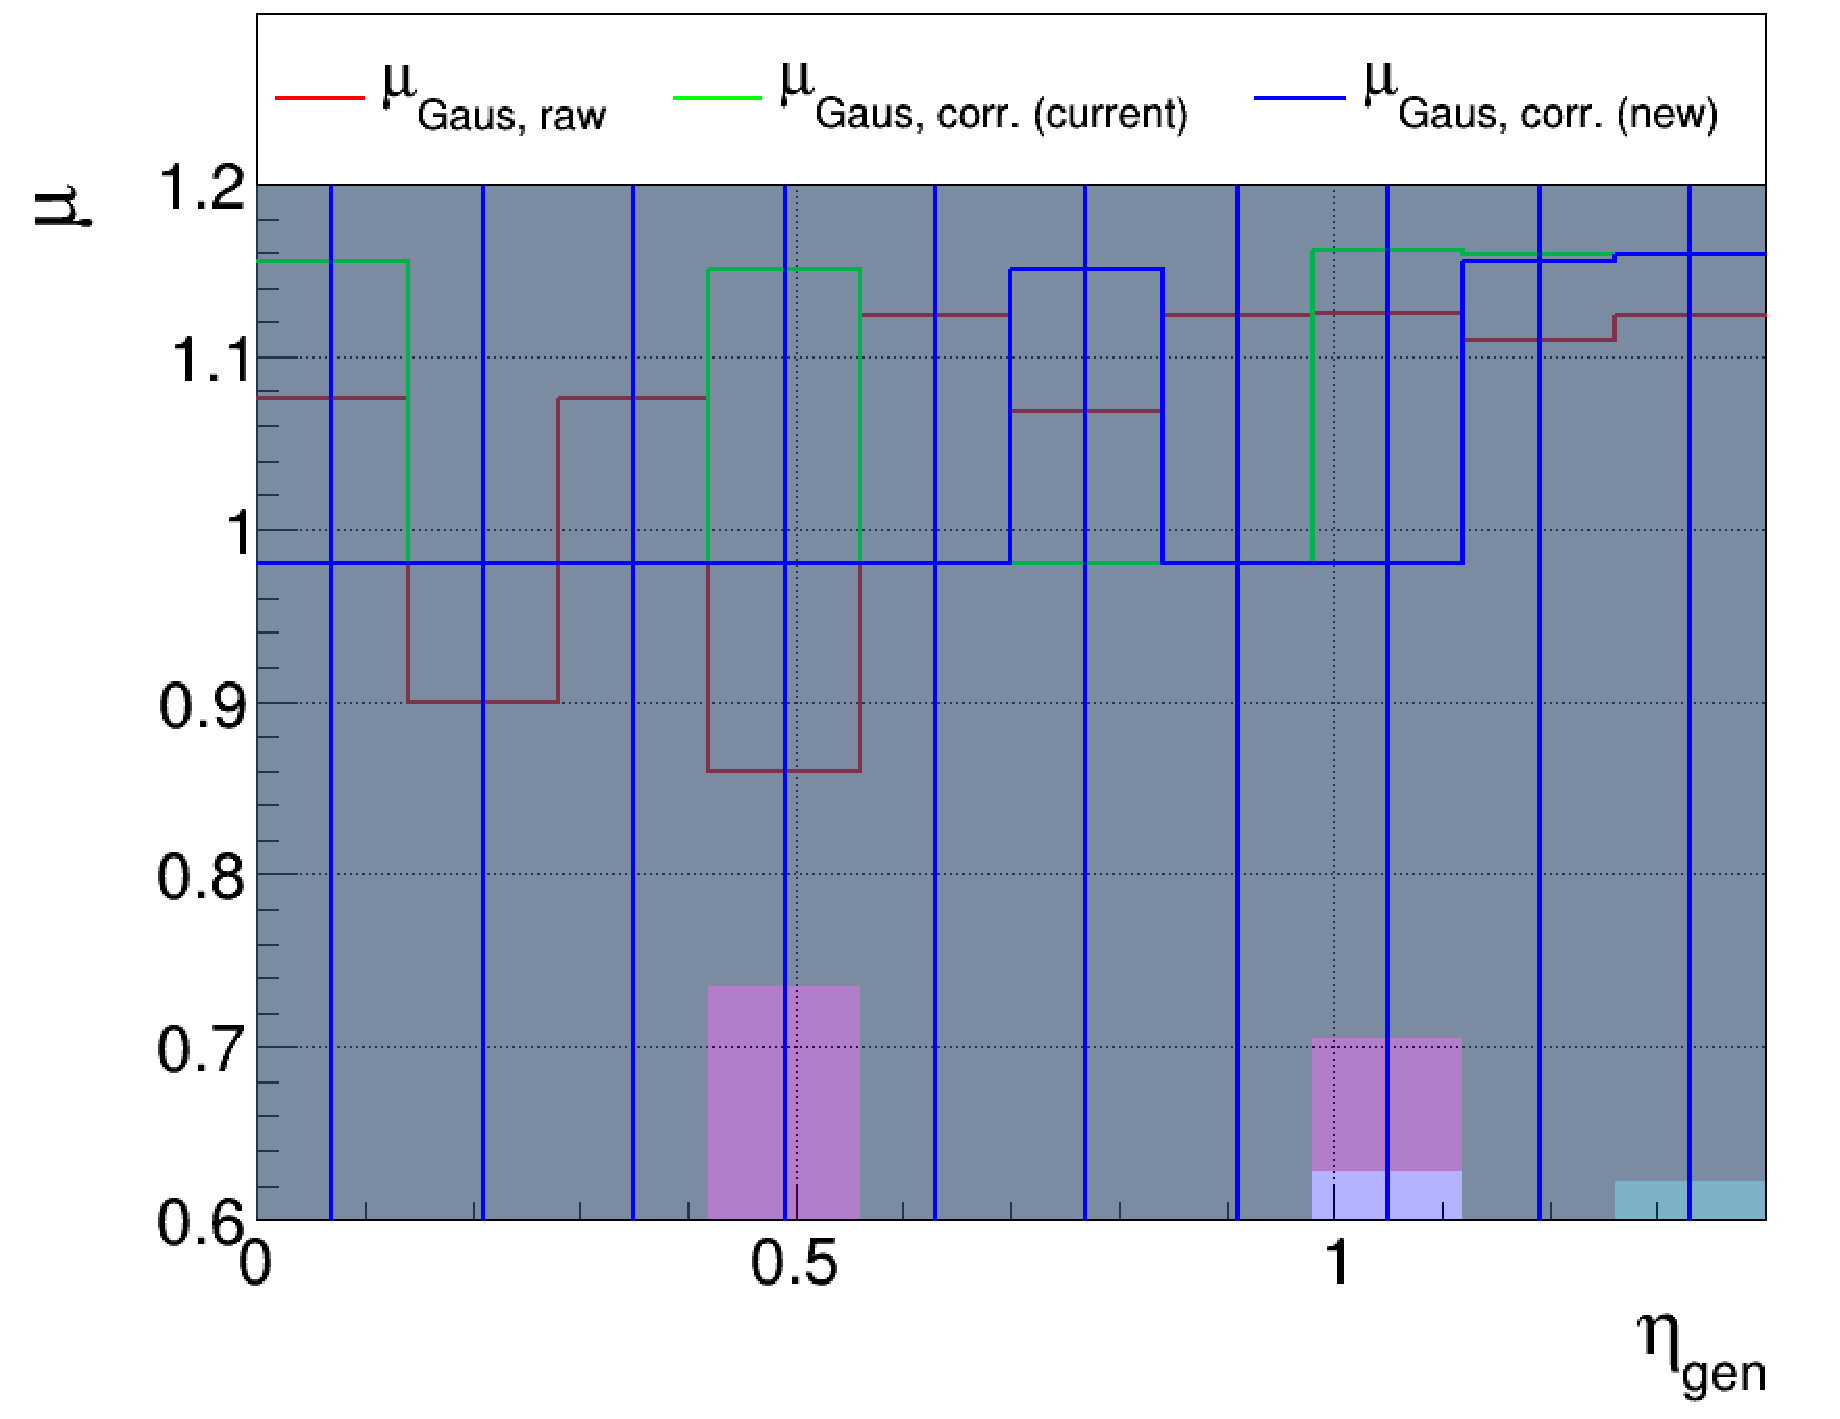
\includegraphics[width=0.495\textwidth]{./plots_pdf/ECAL_plots/plotsPU/EB/ZS/pdf/GENETA/EBZS_GENETA_0006_0025_MuOverBins.pdf}
%% 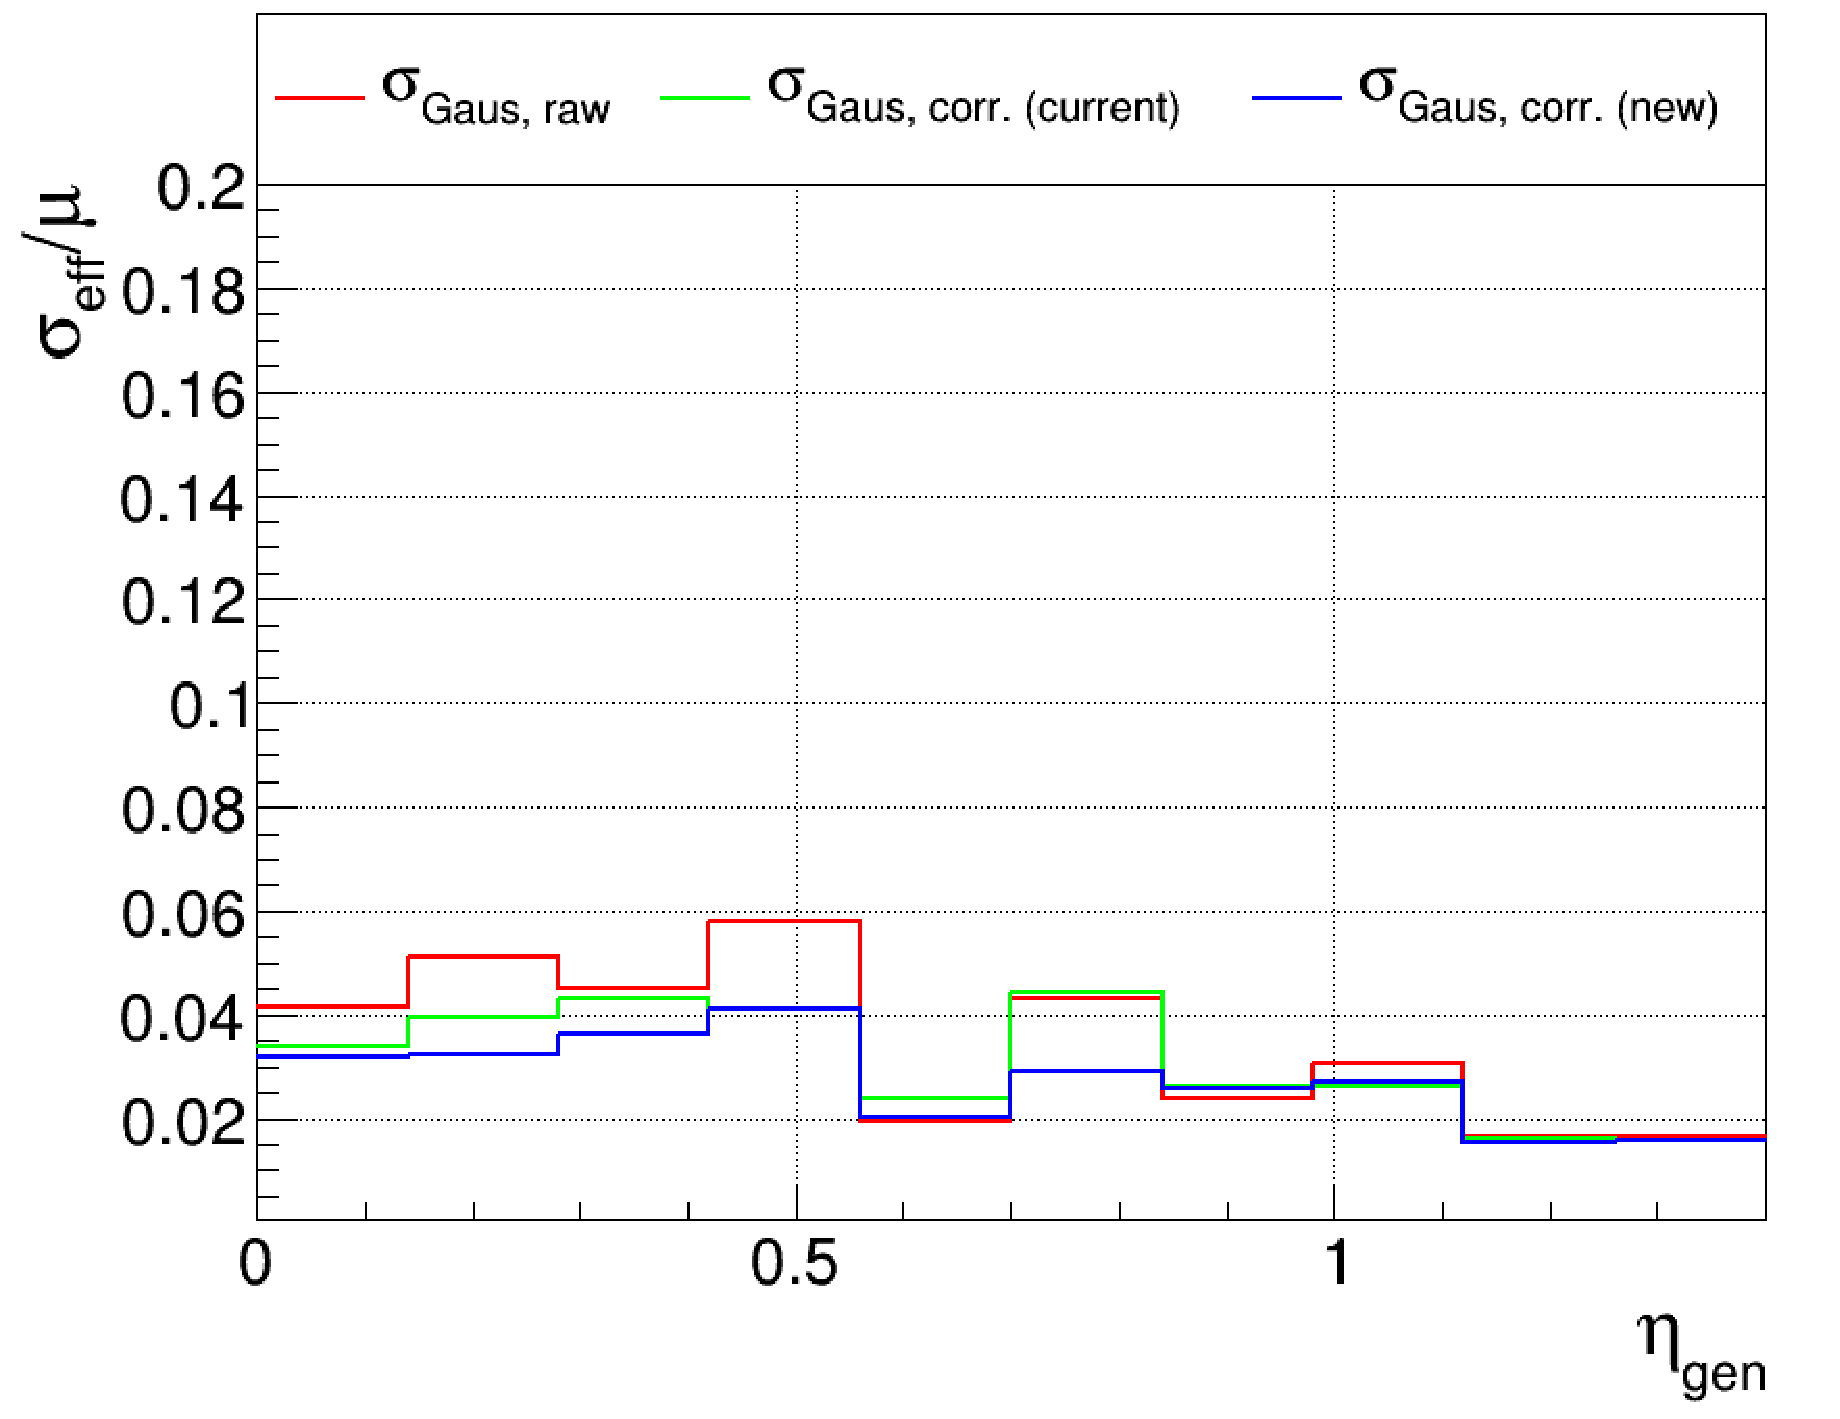
\includegraphics[width=0.495\textwidth]{./plots_pdf/ECAL_plots/plotsPU/EB/ZS/pdf/GENETA/EBZS_GENETA_0006_0025_EffSigmaOverBins.pdf}
%% \caption{EB - ZS Readout \pt 6-25}
%% \end{figure}







\begin{figure}
  %5-20 pt 
\includegraphics[width=0.335\textwidth]{./plots_pdf/ECAL_plots/plotsNOPU/EB/FULL/pdf/GENPT/EBFULL_GENPT_0005_0020_MuOverBins.pdf}
\includegraphics[width=0.3355\textwidth]{./plots_pdf/ECAL_plots/plotsNOPU/EB/FULL/pdf/GENPT/EBFULL_GENPT_0005_0020_EffSigmaOverBins.pdf}

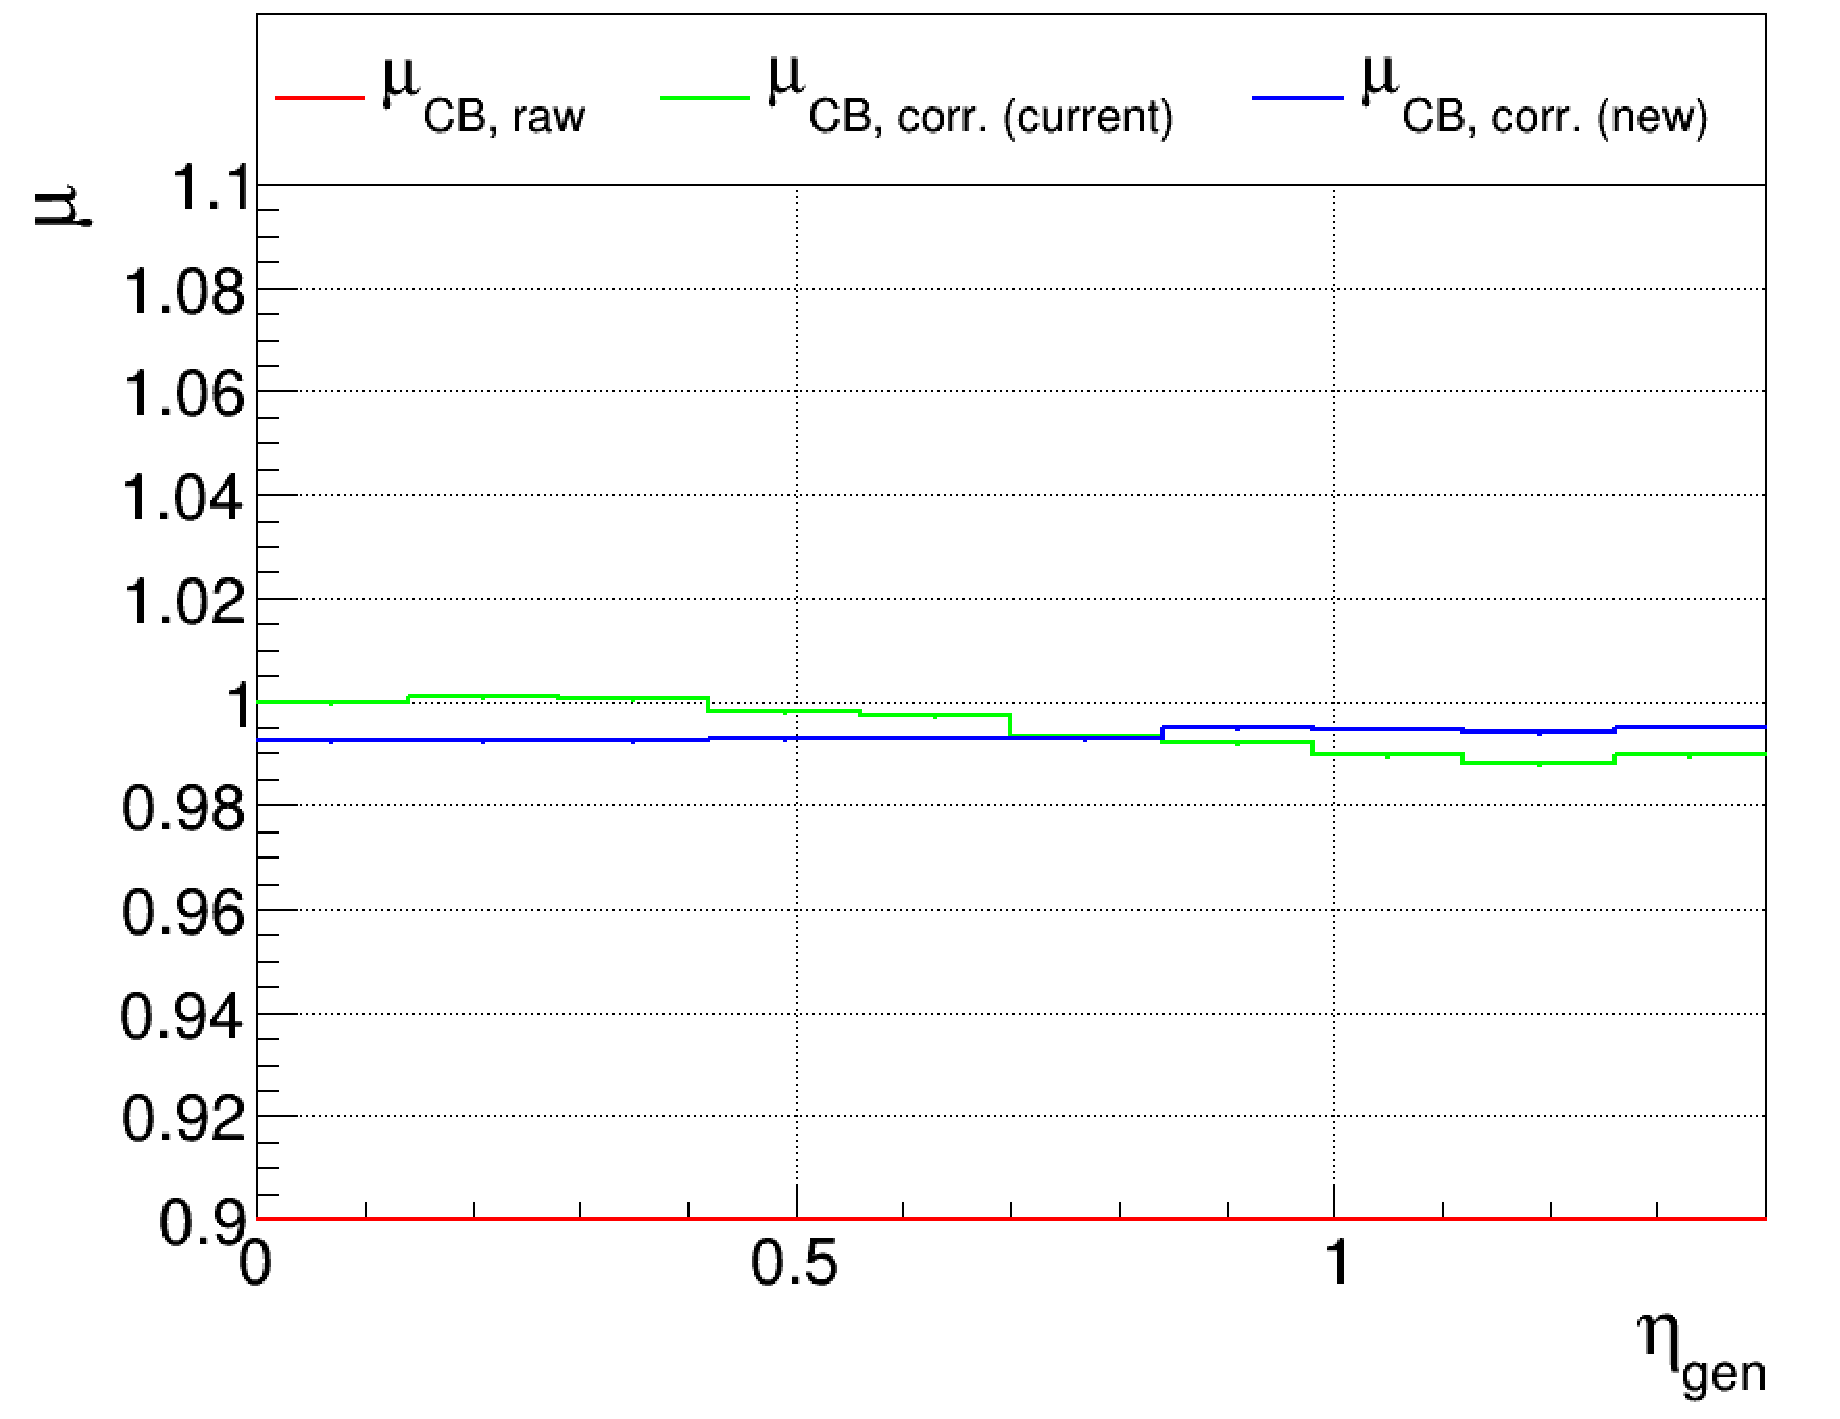
\includegraphics[width=0.495\textwidth]{./plots_pdf/ECAL_plots/plotsNOPU/EB/FULL/pdf/GENETA/EBFULL_GENETA_0005_0020_MuOverBins.pdf}
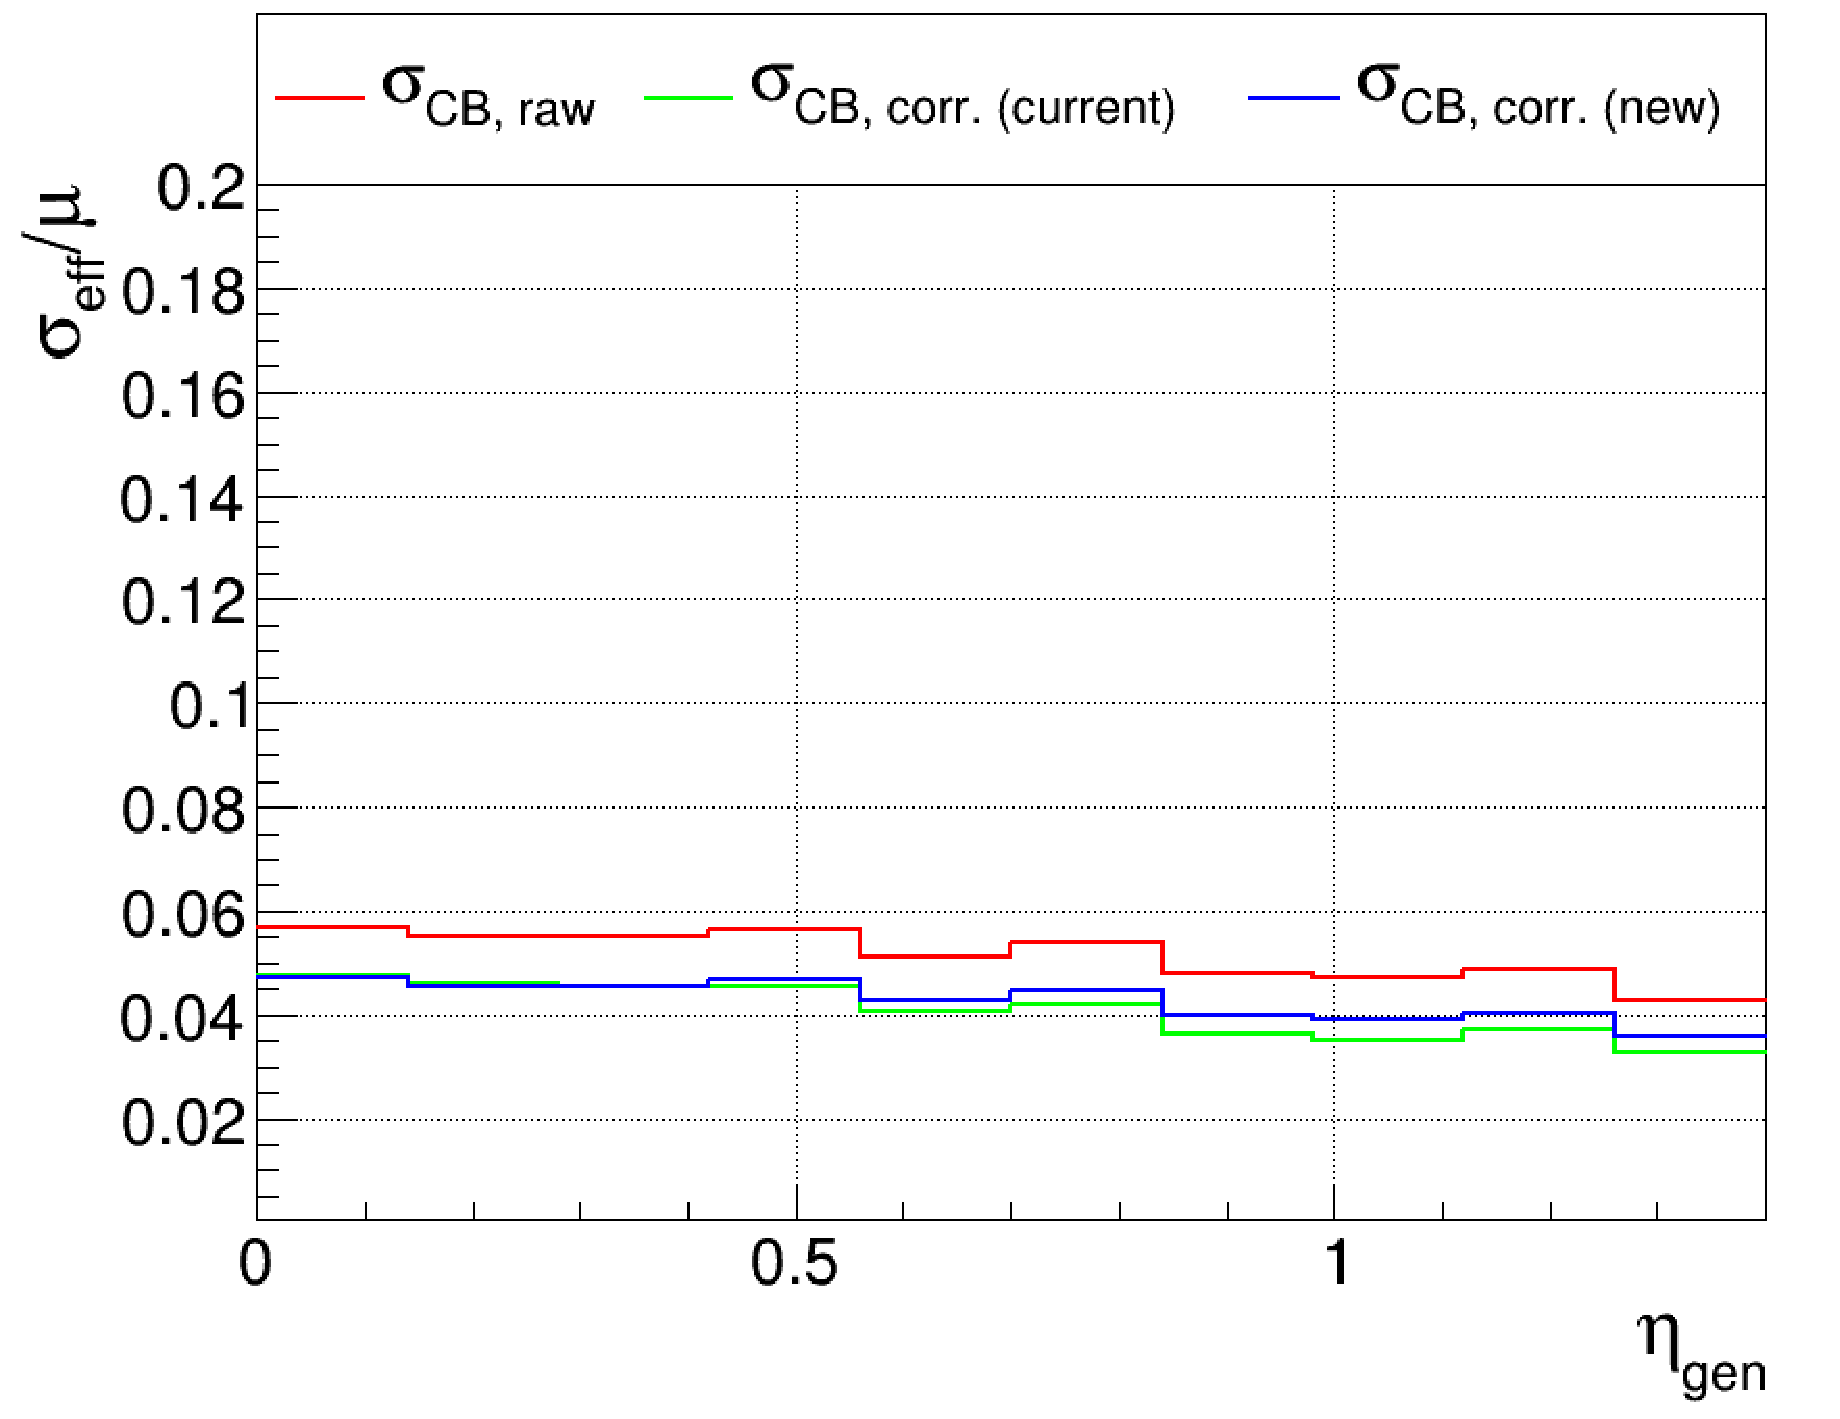
\includegraphics[width=0.495\textwidth]{./plots_pdf/ECAL_plots/plotsPU/EB/FULL/pdf/GENETA/EBFULL_GENETA_0005_0020_EffSigmaOverBins.pdf}
\caption{EB - Full Readout \pt 5-20}

%\begin{figure}
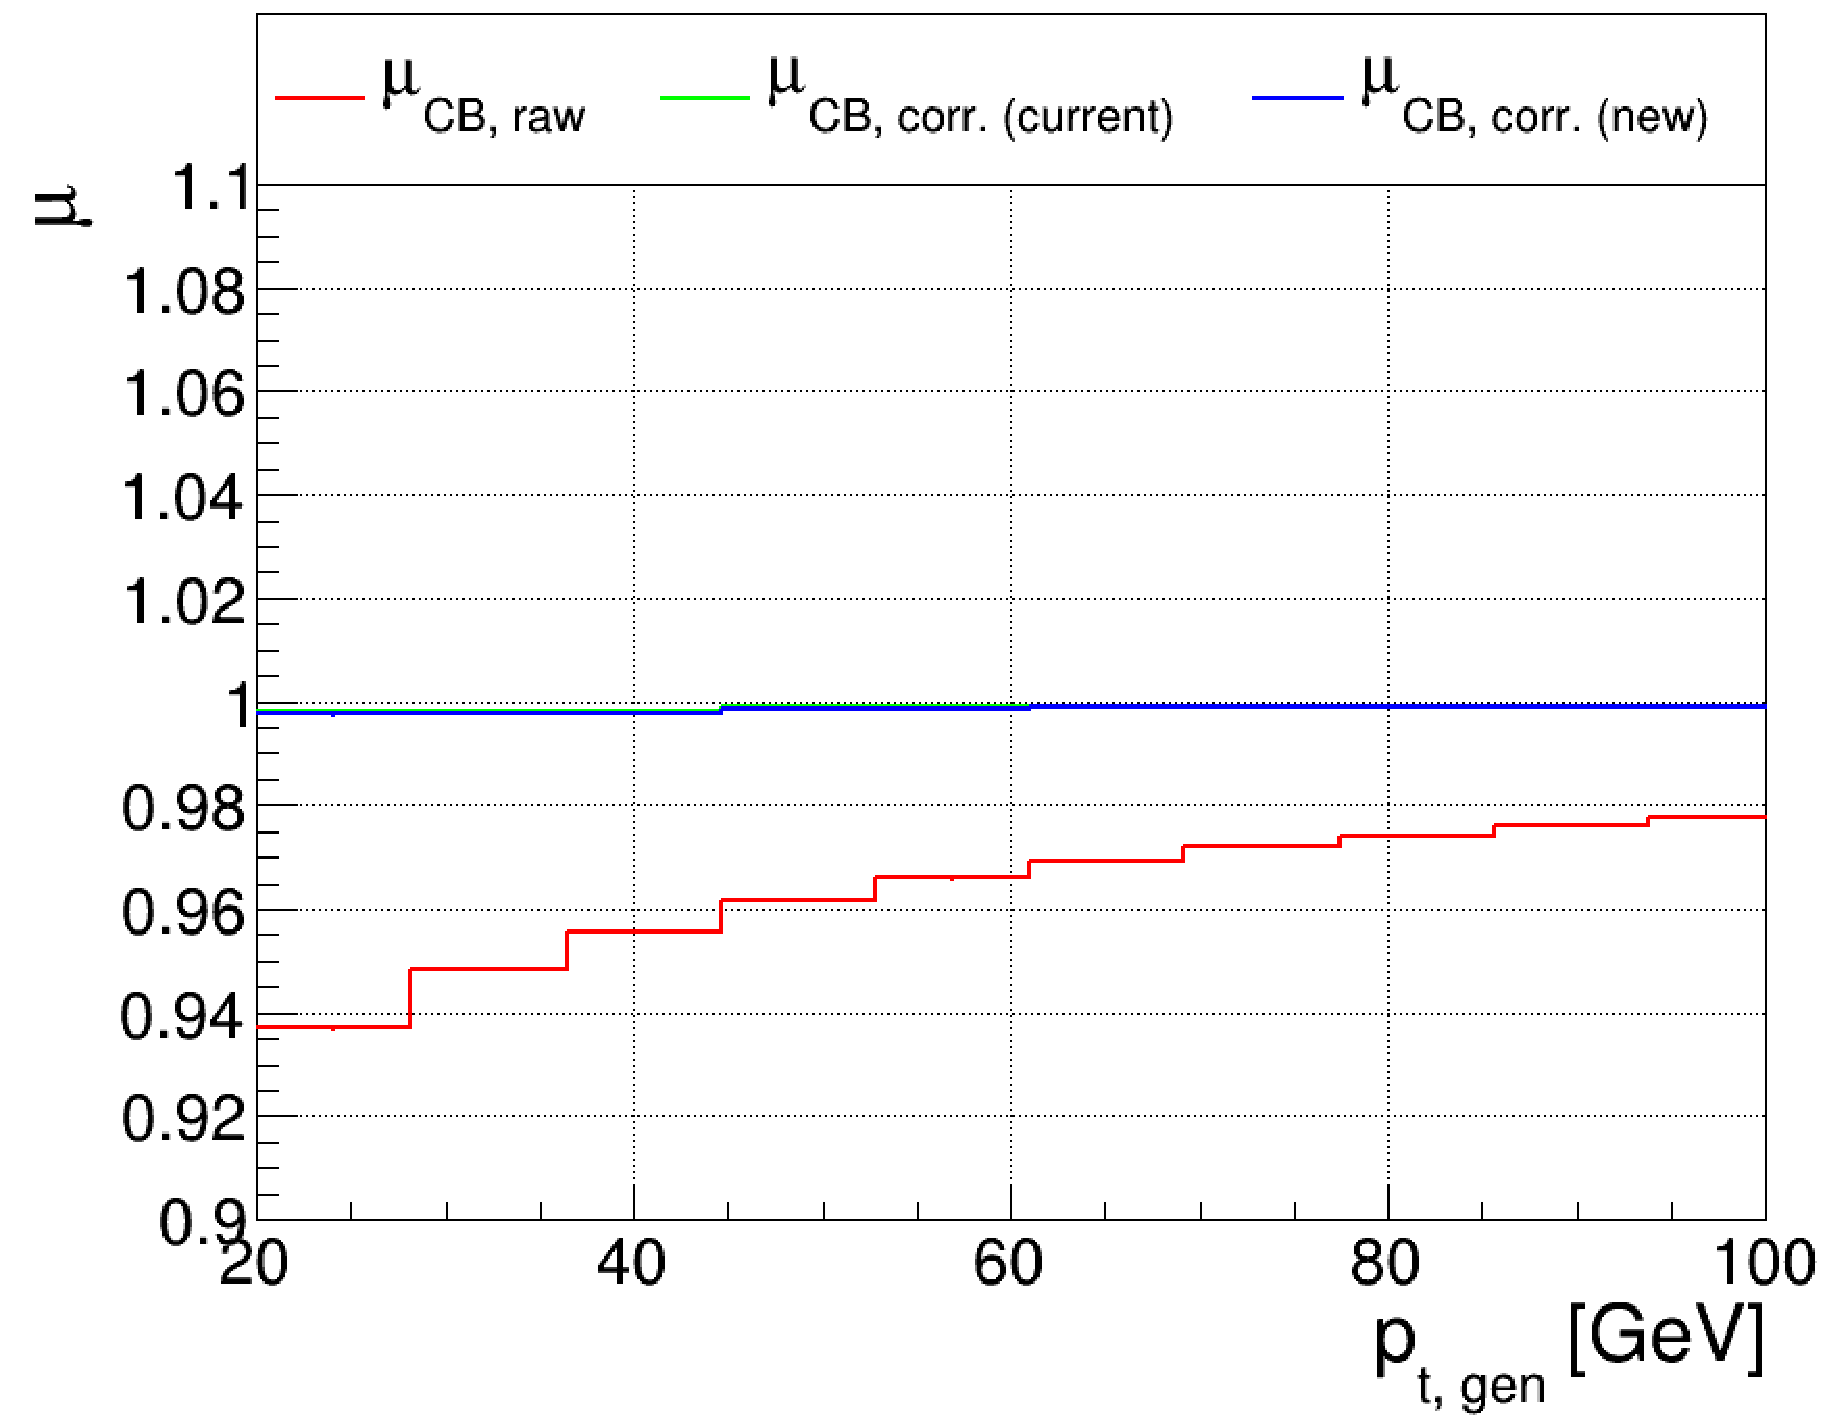
\includegraphics[width=0.495\textwidth]{./plots_pdf/ECAL_plots/plotsNOPU/EB/FULL/pdf/GENPT/EBFULL_GENPT_0020_0100_MuOverBins.pdf}
\includegraphics[width=0.495\textwidth]{./plots_pdf/ECAL_plots/plotsNOPU/EB/FULL/pdf/GENPT/EBFULL_GENPT_0020_0100_EffSigmaOverBins.pdf}

\includegraphics[width=0.495\textwidth]{./plots_pdf/ECAL_plots/plotsNOPU/EB/FULL/pdf/GENETA/EBFULL_GENETA_0020_0100_MuOverBins.pdf}
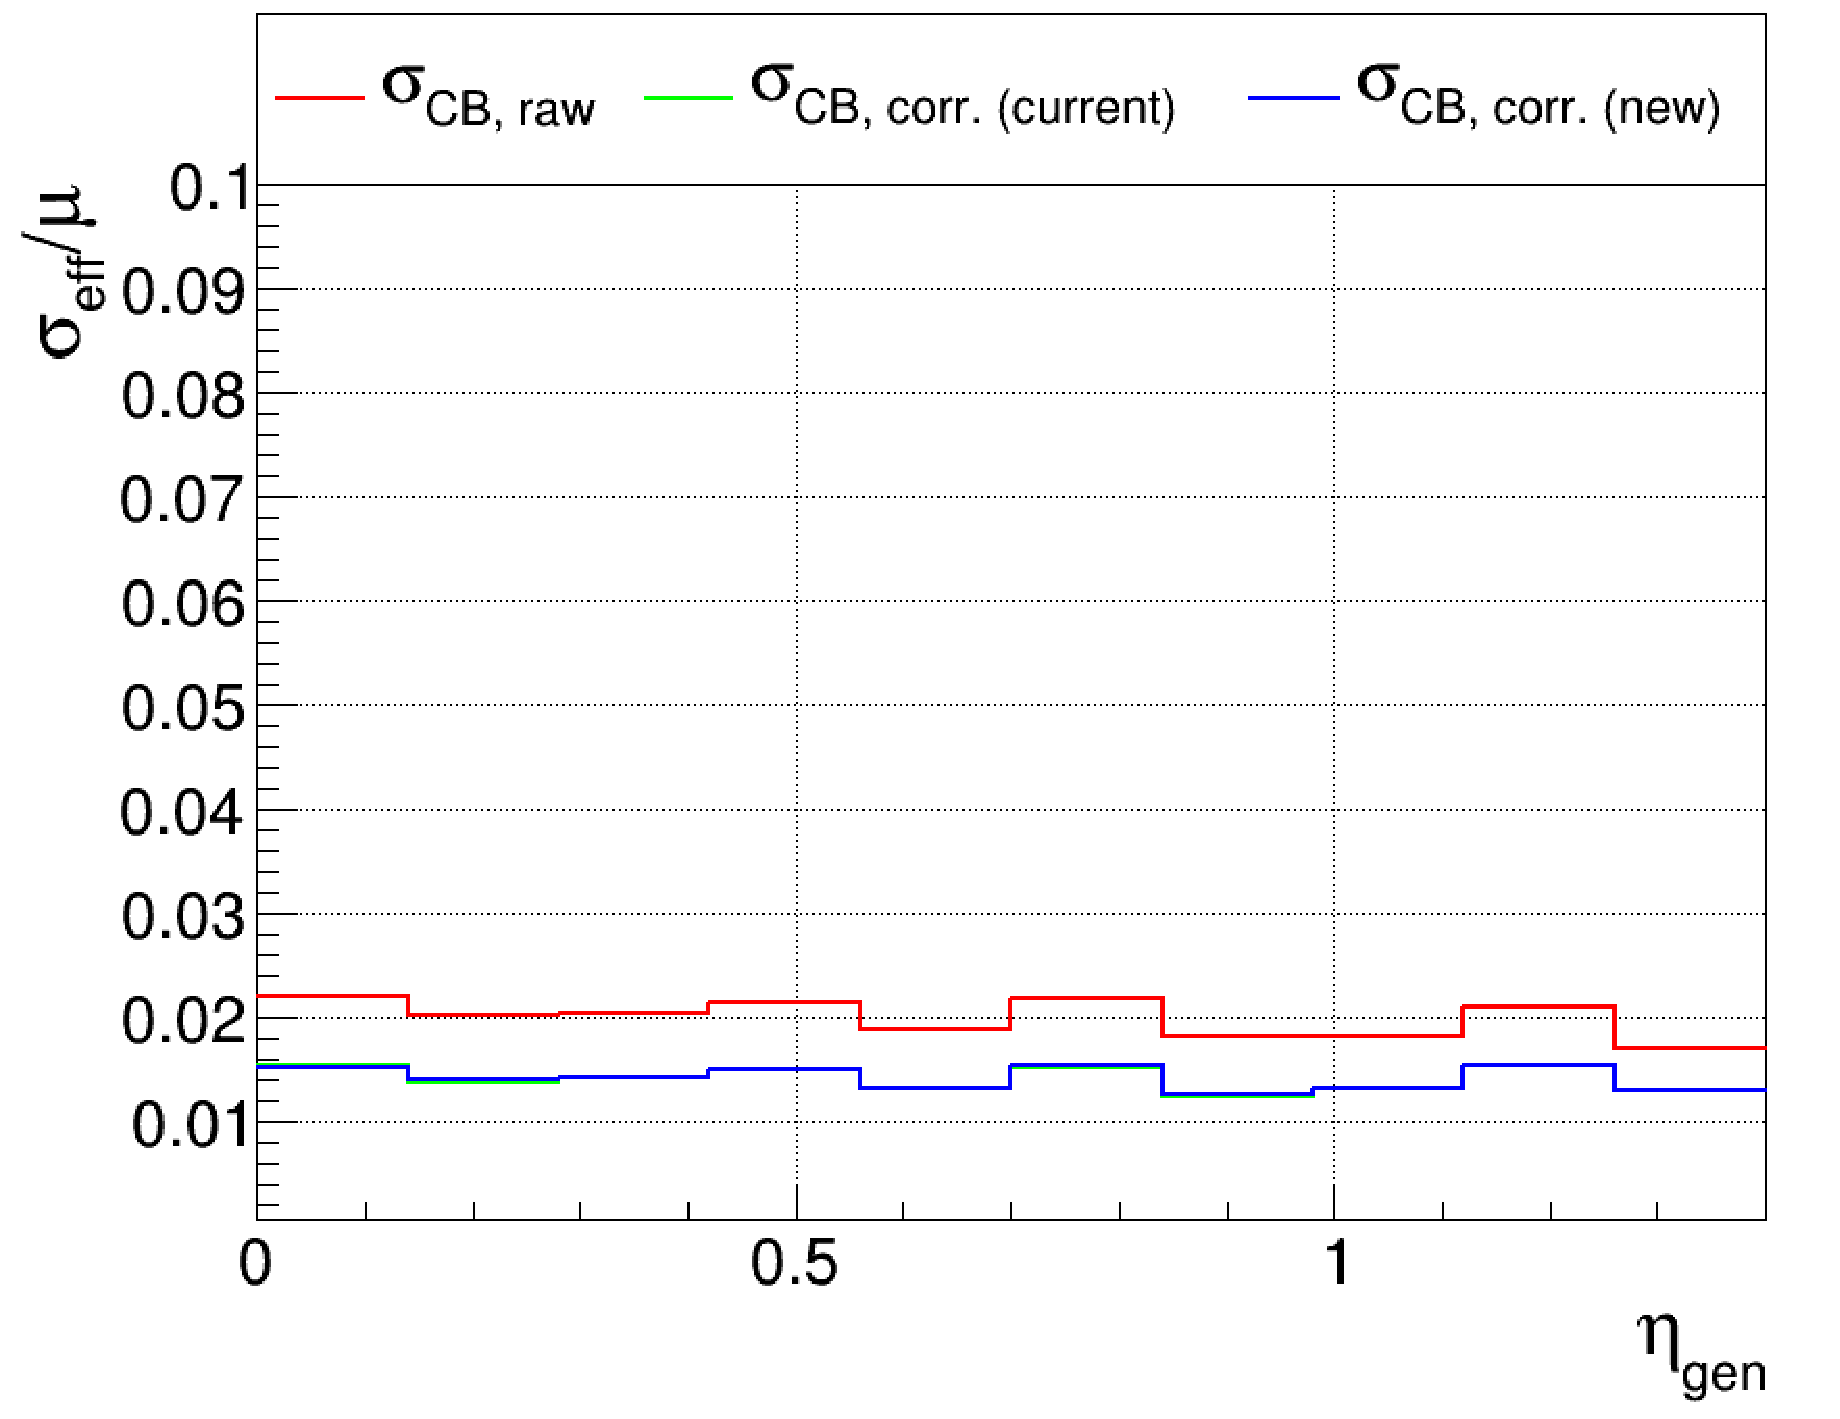
\includegraphics[width=0.495\textwidth]{./plots_pdf/ECAL_plots/plotsPU/EB/FULL/pdf/GENETA/EBFULL_GENETA_0020_0100_EffSigmaOverBins.pdf}
\caption{EB - Full Readout \pt 20-100}
\end{figure}


\begin{figure}
\includegraphics[width=0.495\textwidth]{./plots_pdf/ECAL_plots/plotsNOPU/EB/FULL/pdf/GENPT/EBFULL_GENPT_0100_0300_MuOverBins.pdf}
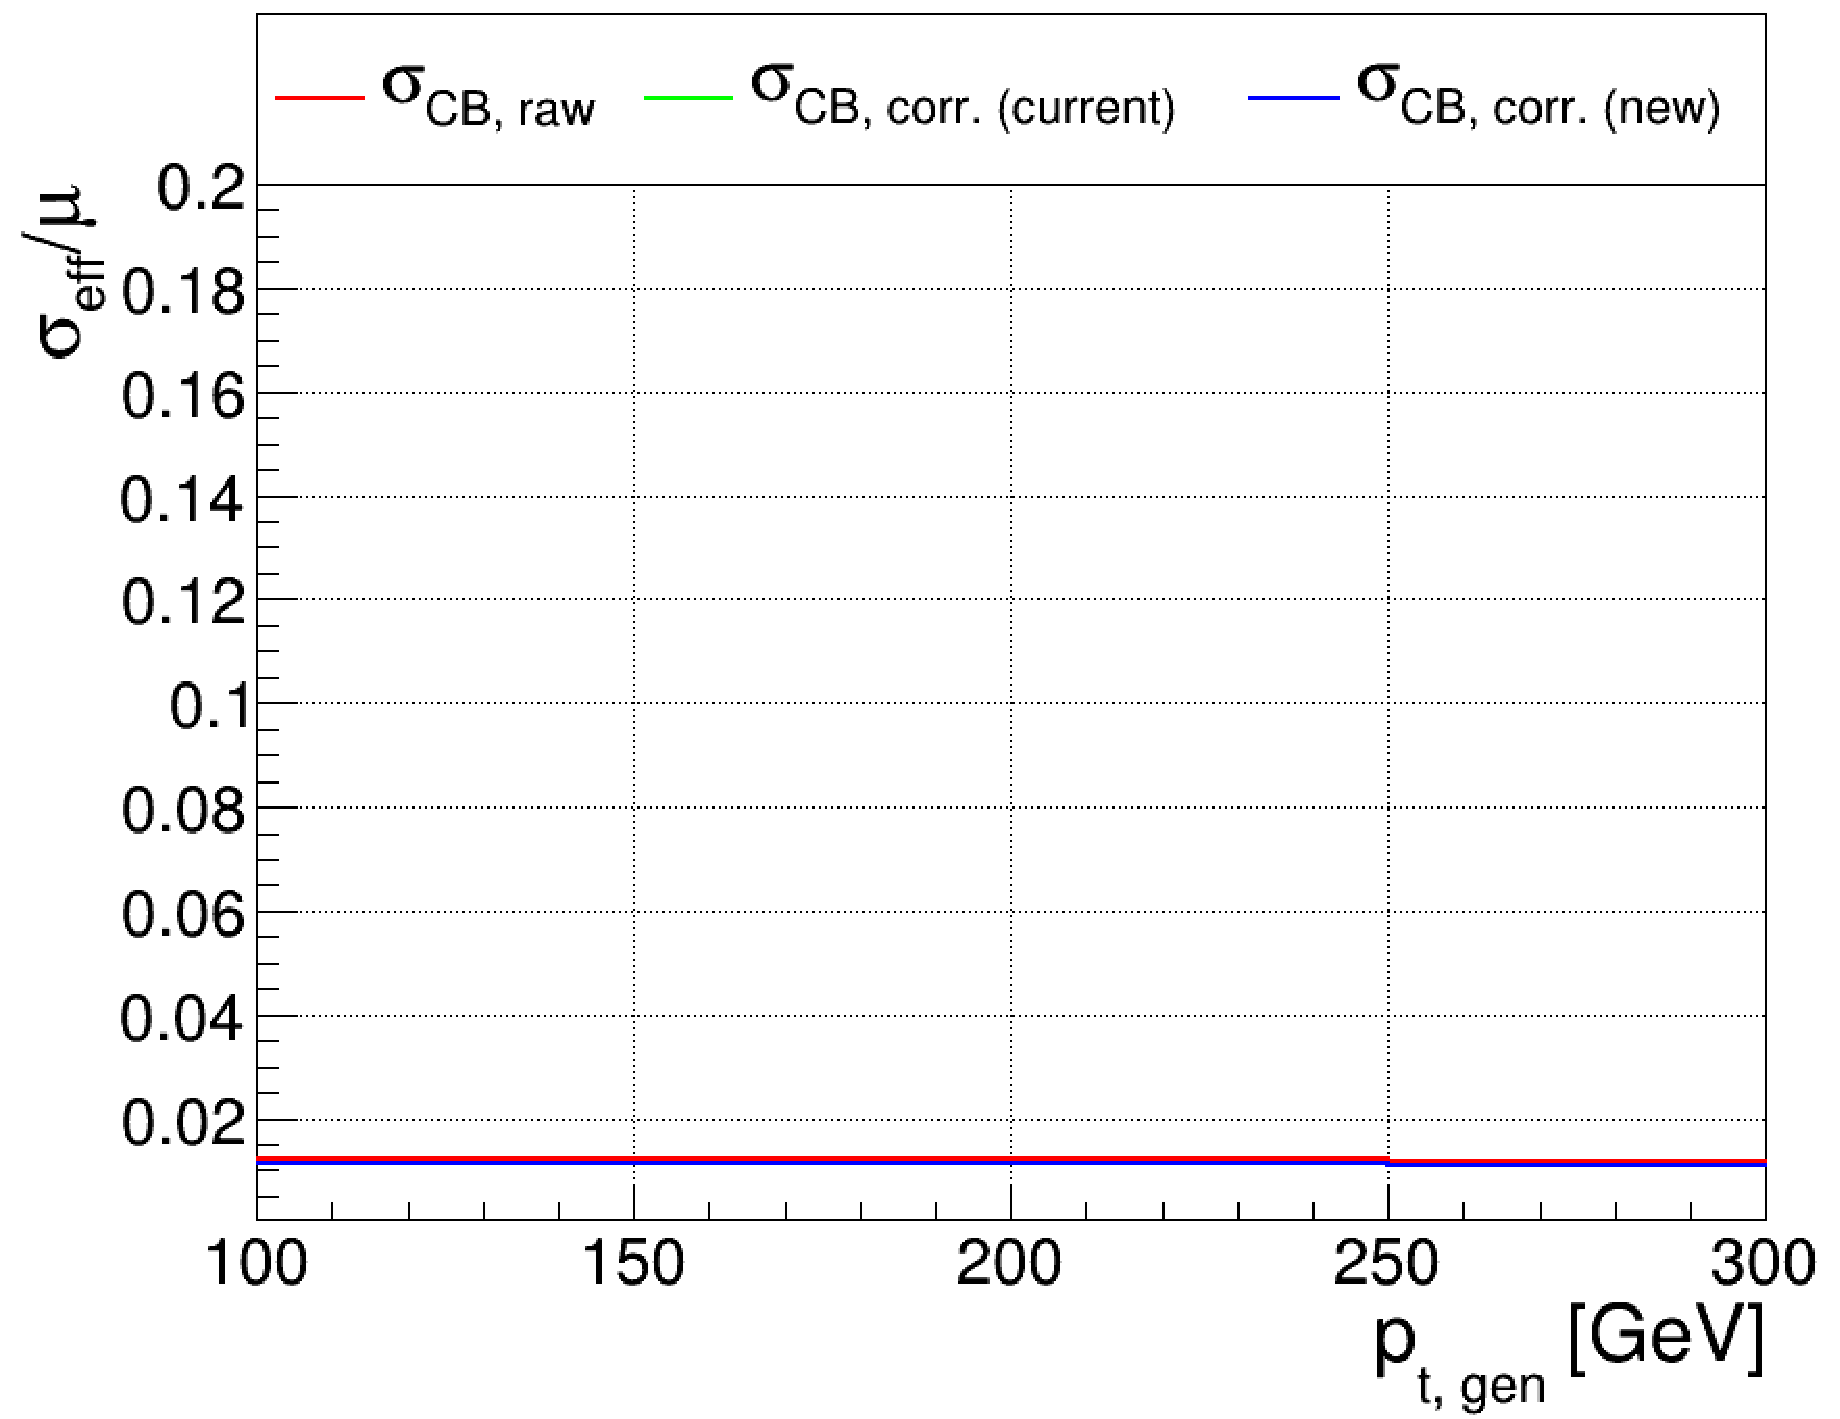
\includegraphics[width=0.495\textwidth]{./plots_pdf/ECAL_plots/plotsPU/EB/FULL/pdf/GENPT/EBFULL_GENPT_0100_0300_EffSigmaOverBins.pdf}


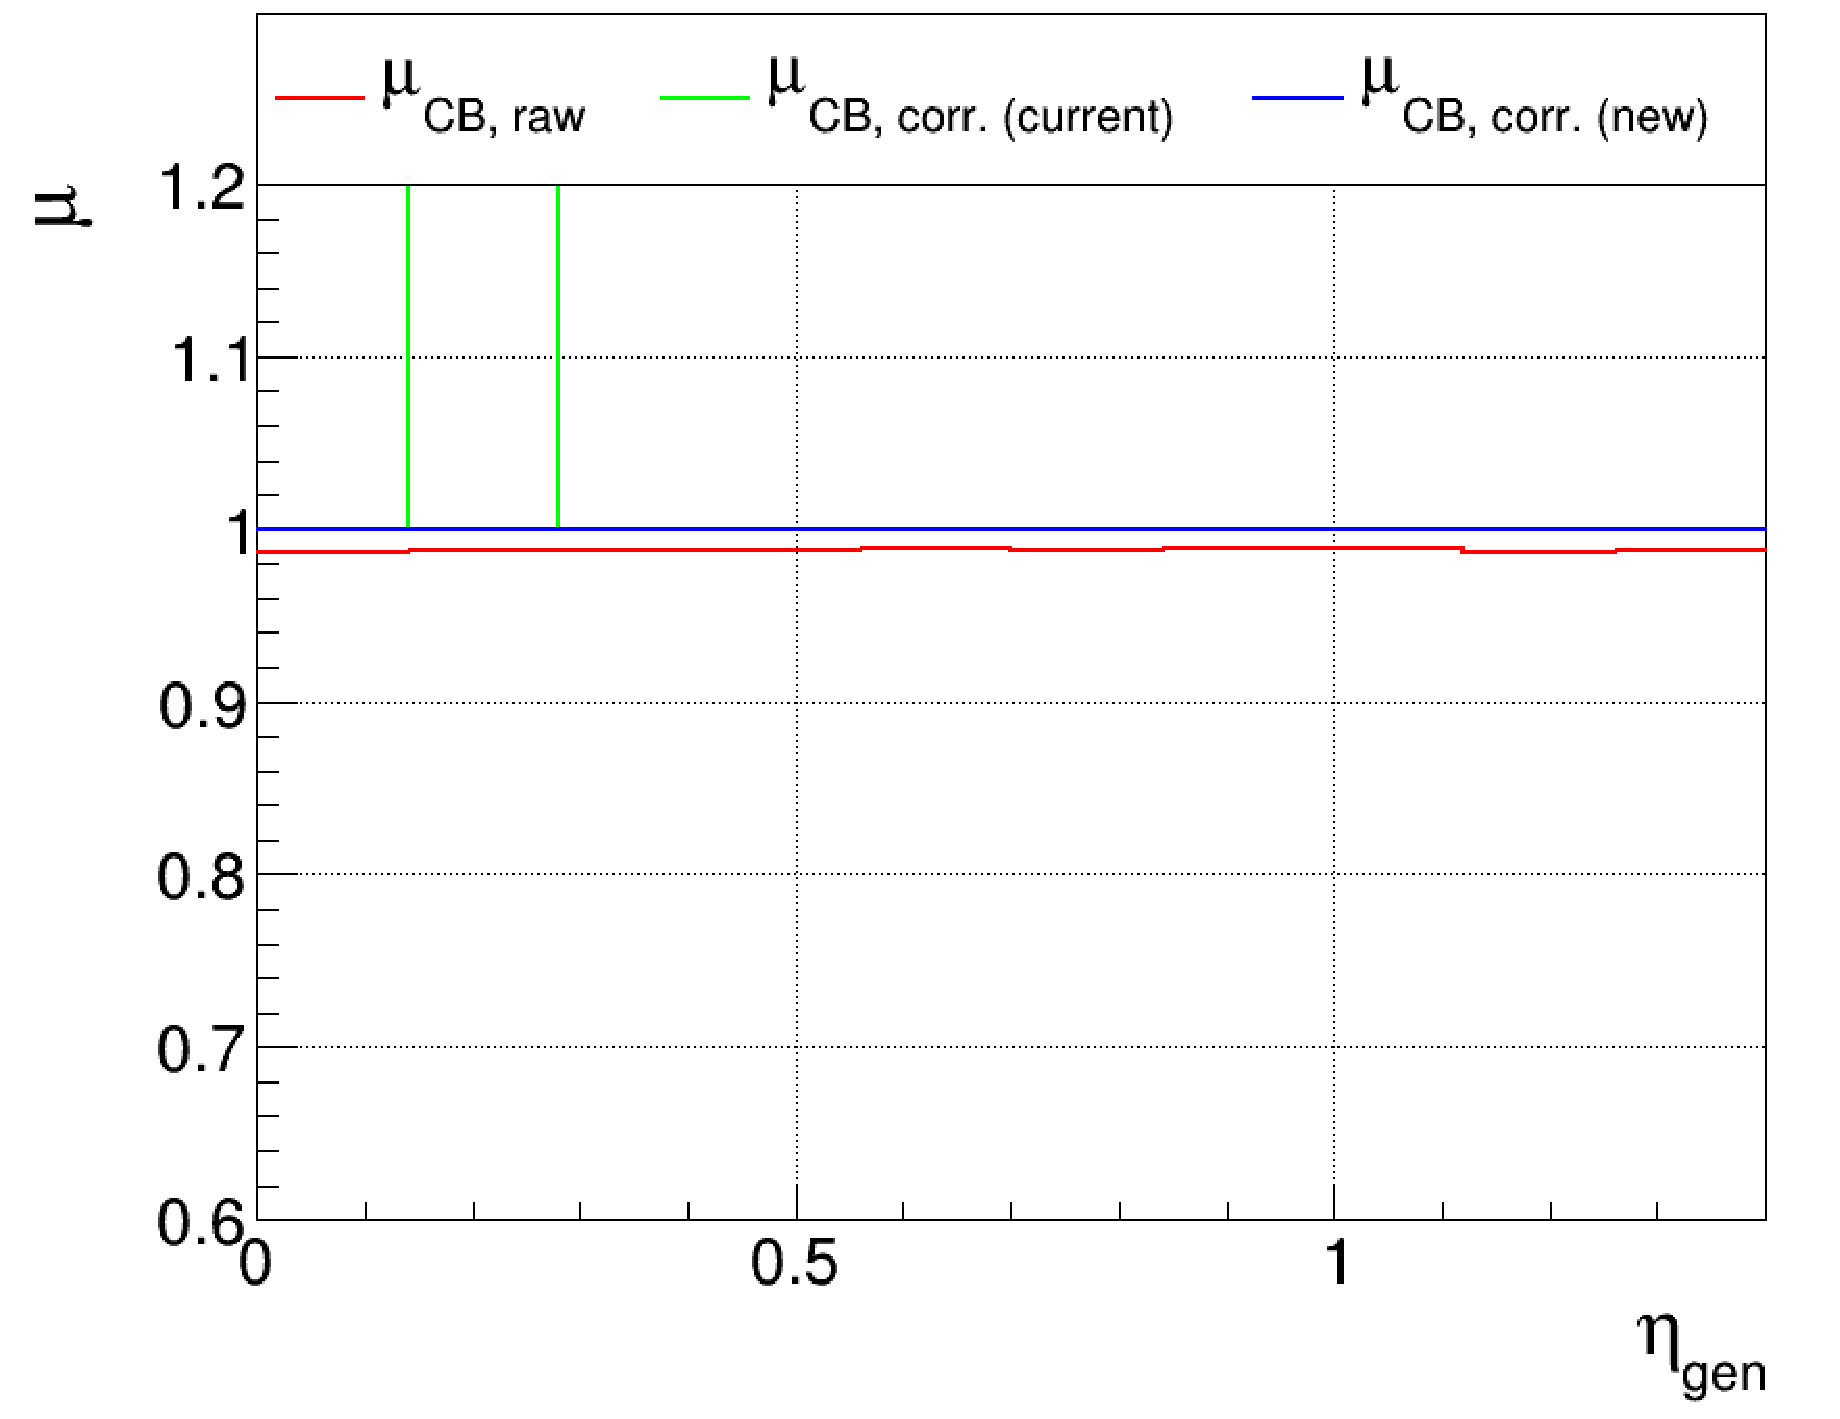
\includegraphics[width=0.495\textwidth]{./plots_pdf/ECAL_plots/plotsNOPU/EB/FULL/pdf/GENETA/EBFULL_GENETA_0100_0300_MuOverBins.pdf}
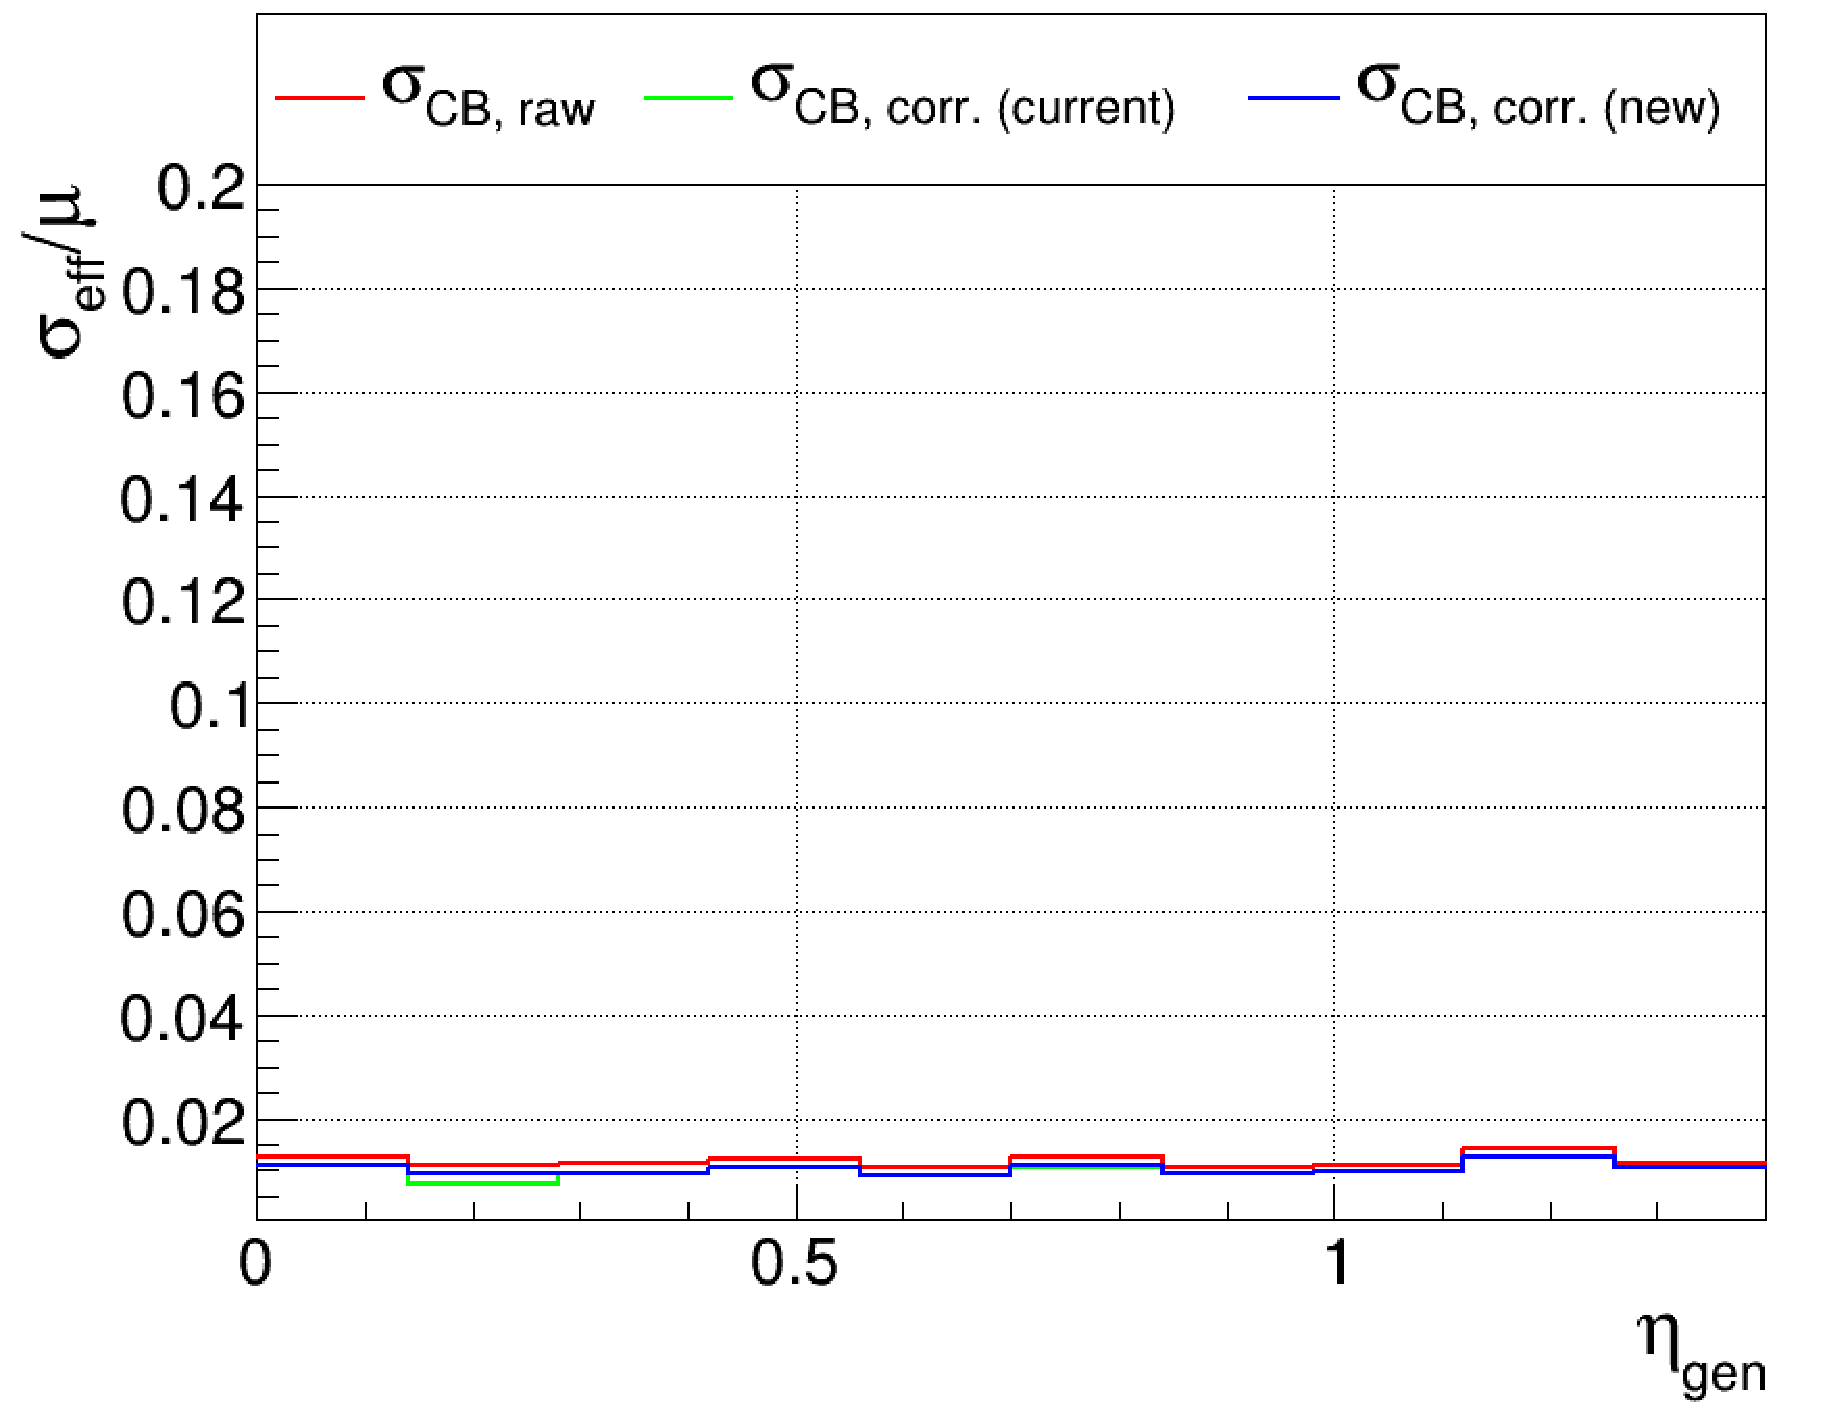
\includegraphics[width=0.495\textwidth]{./plots_pdf/ECAL_plots/plotsNOPU/EB/FULL/pdf/GENETA/EBFULL_GENETA_0100_0300_EffSigmaOverBins.pdf}
\caption{EB - Full Readout \pt 100-300}
\end{figure}




\begin{figure}
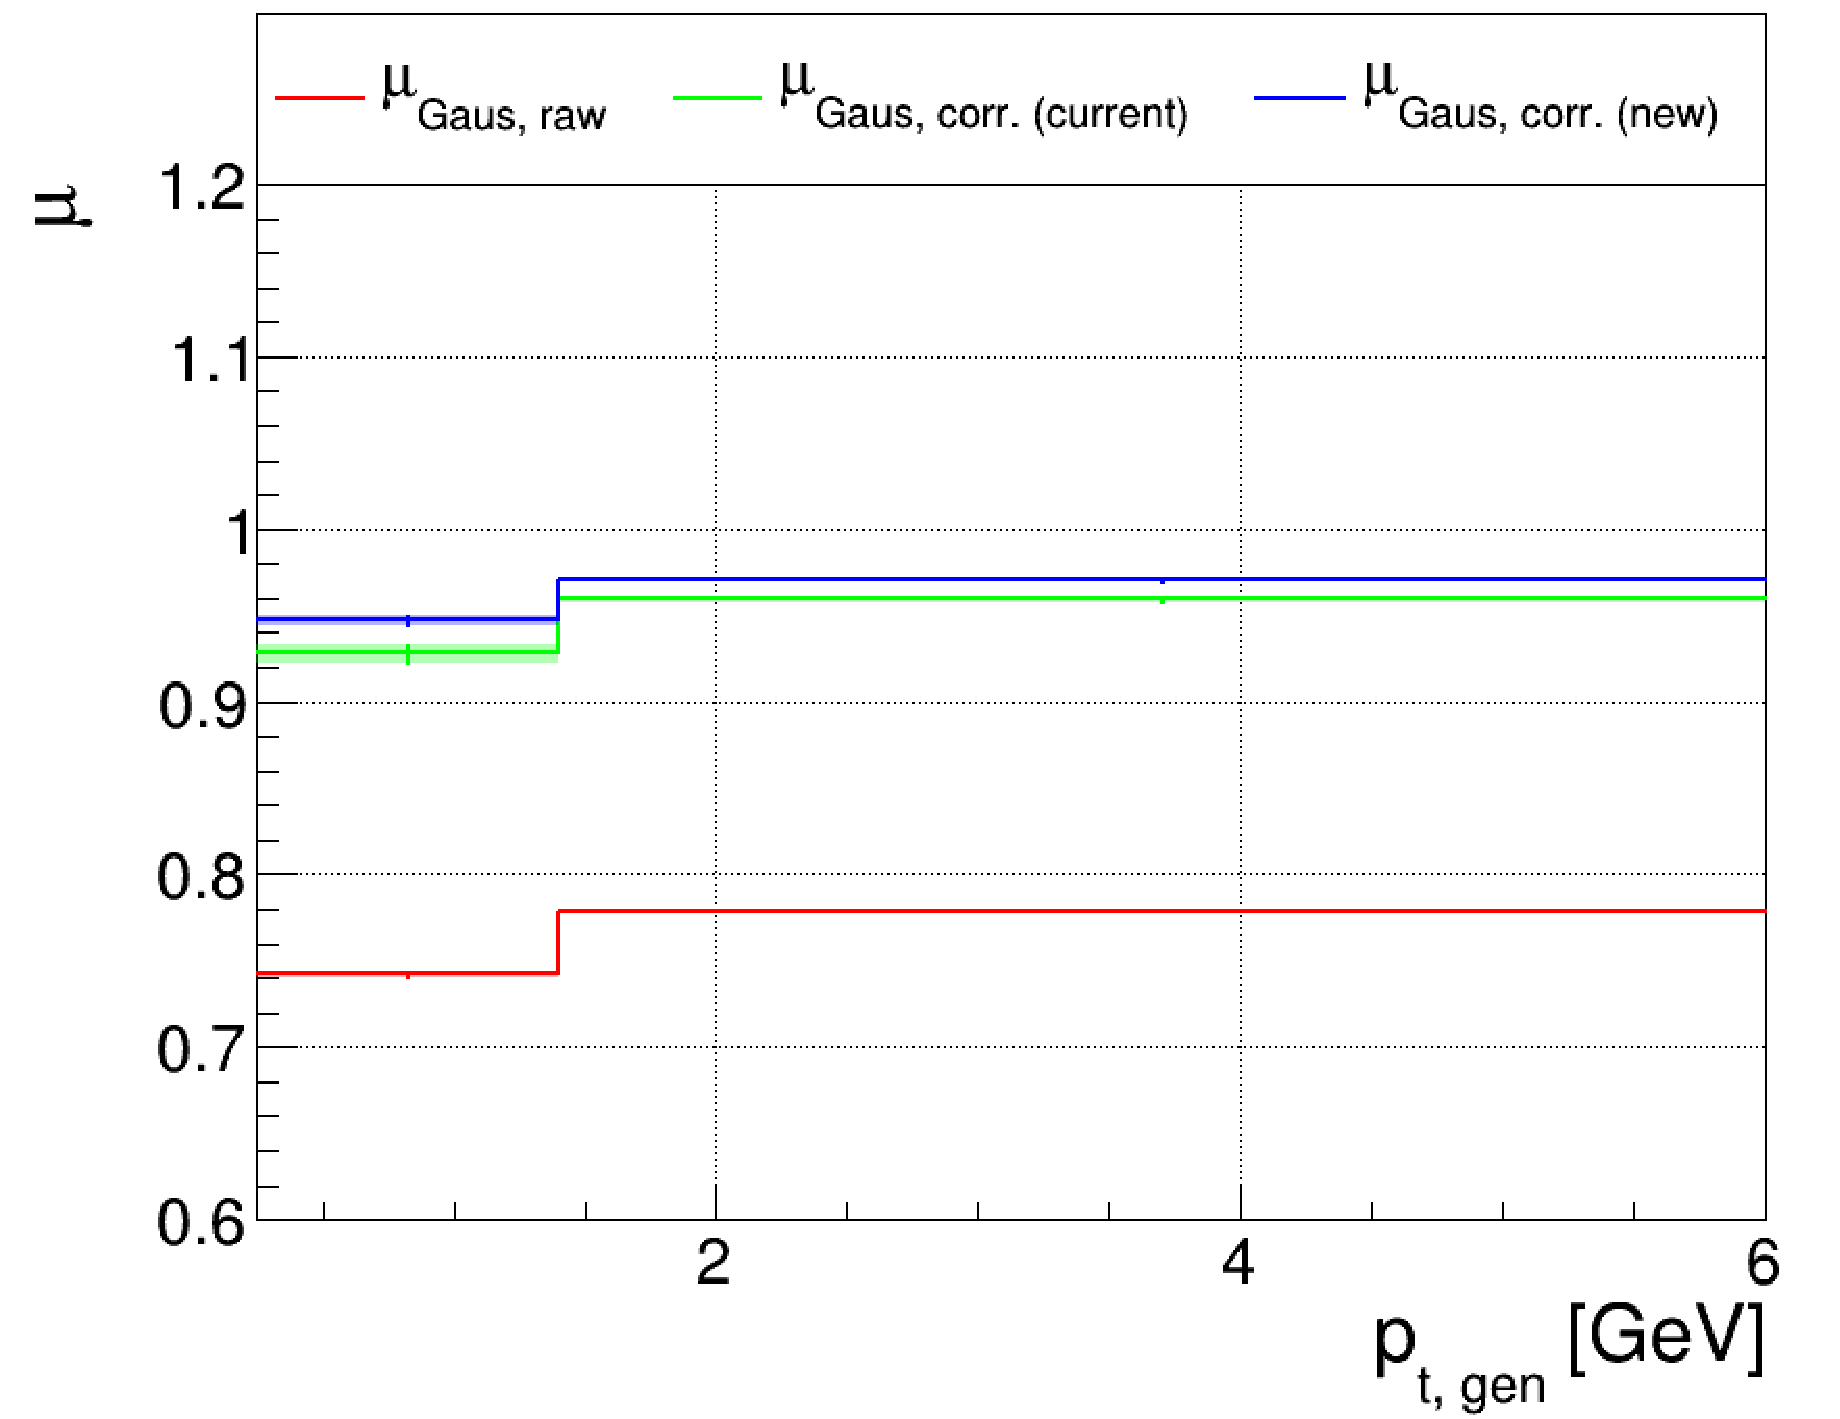
\includegraphics[width=0.495\textwidth]{./ECAL_plots/plotsNOPU/EB/ZS/pdf/GENPT/EBZS_GENPT_0000_0006_MuOverBins.pdf}
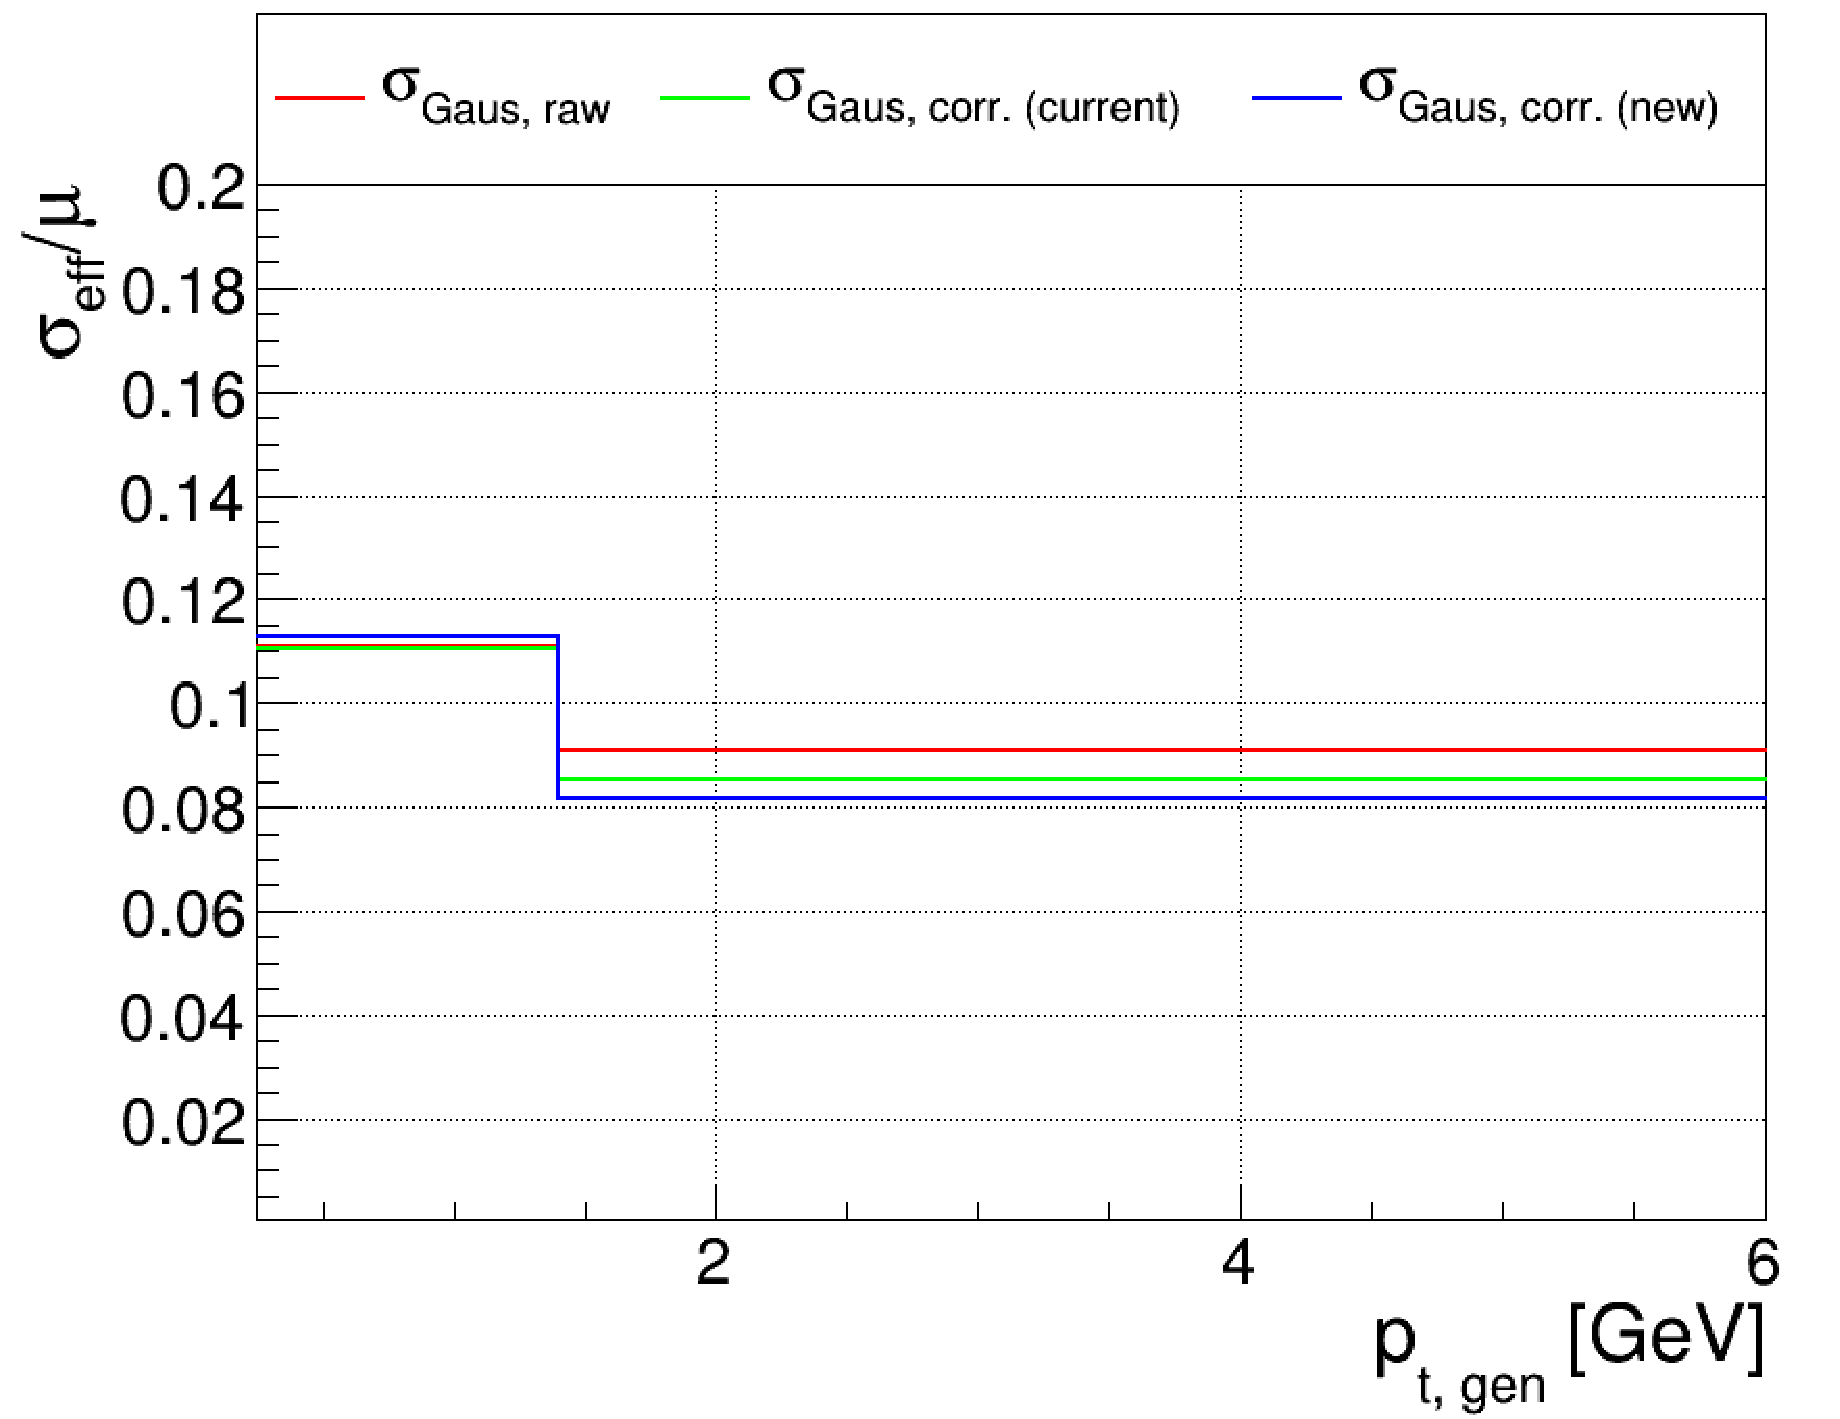
\includegraphics[width=0.495\textwidth]{./ECAL_plots/plotsNOPU/EB/ZS/pdf/GENPT/EBZS_GENPT_0000_0006_EffSigmaOverBins.pdf}
%\caption{EB - ZSl Readout pt 0-6}
%\end{figure}
%\begin{figure}
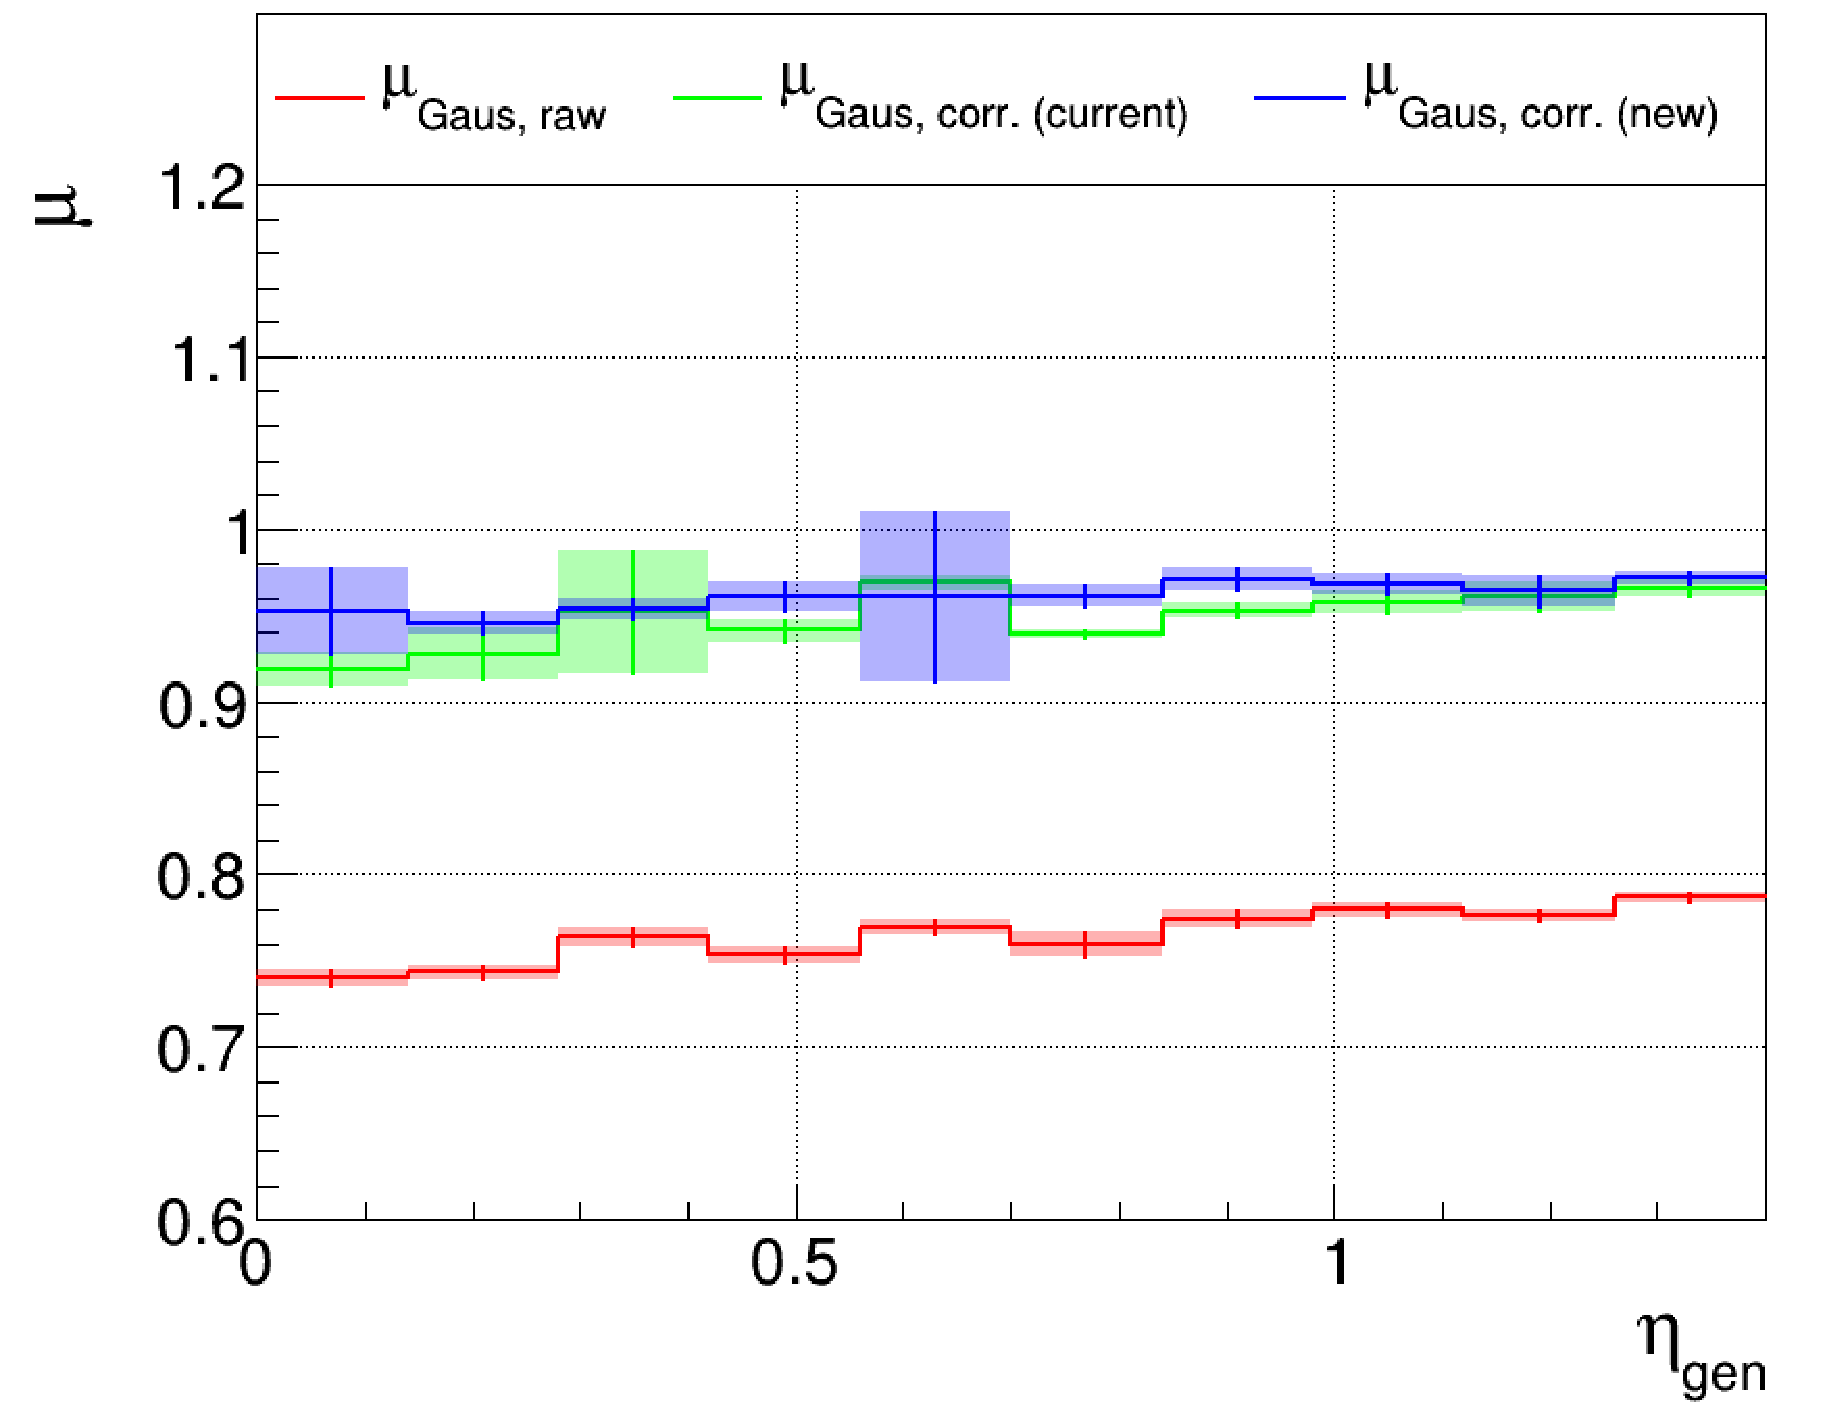
\includegraphics[width=0.495\textwidth]{./ECAL_plots/plotsNOPU/EB/ZS/pdf/GENETA/EBZS_GENETA_0000_0006_MuOverBins.pdf}
\includegraphics[width=0.495\textwidth]{./ECAL_plots/plotsNOPU/EB/ZS/pdf/GENETA/EBZS_GENETA_0000_0006_EffSigmaOverBins.pdf}
\caption{EB - ZS Readout pt 0-6}
\end{figure}


\begin{figure}
\includegraphics[width=0.495\textwidth]{./ECAL_plots/plotsNOPU/EB/ZS/pdf/GENPT/EBZS_GENPT_0006_0025_MuOverBins.pdf}
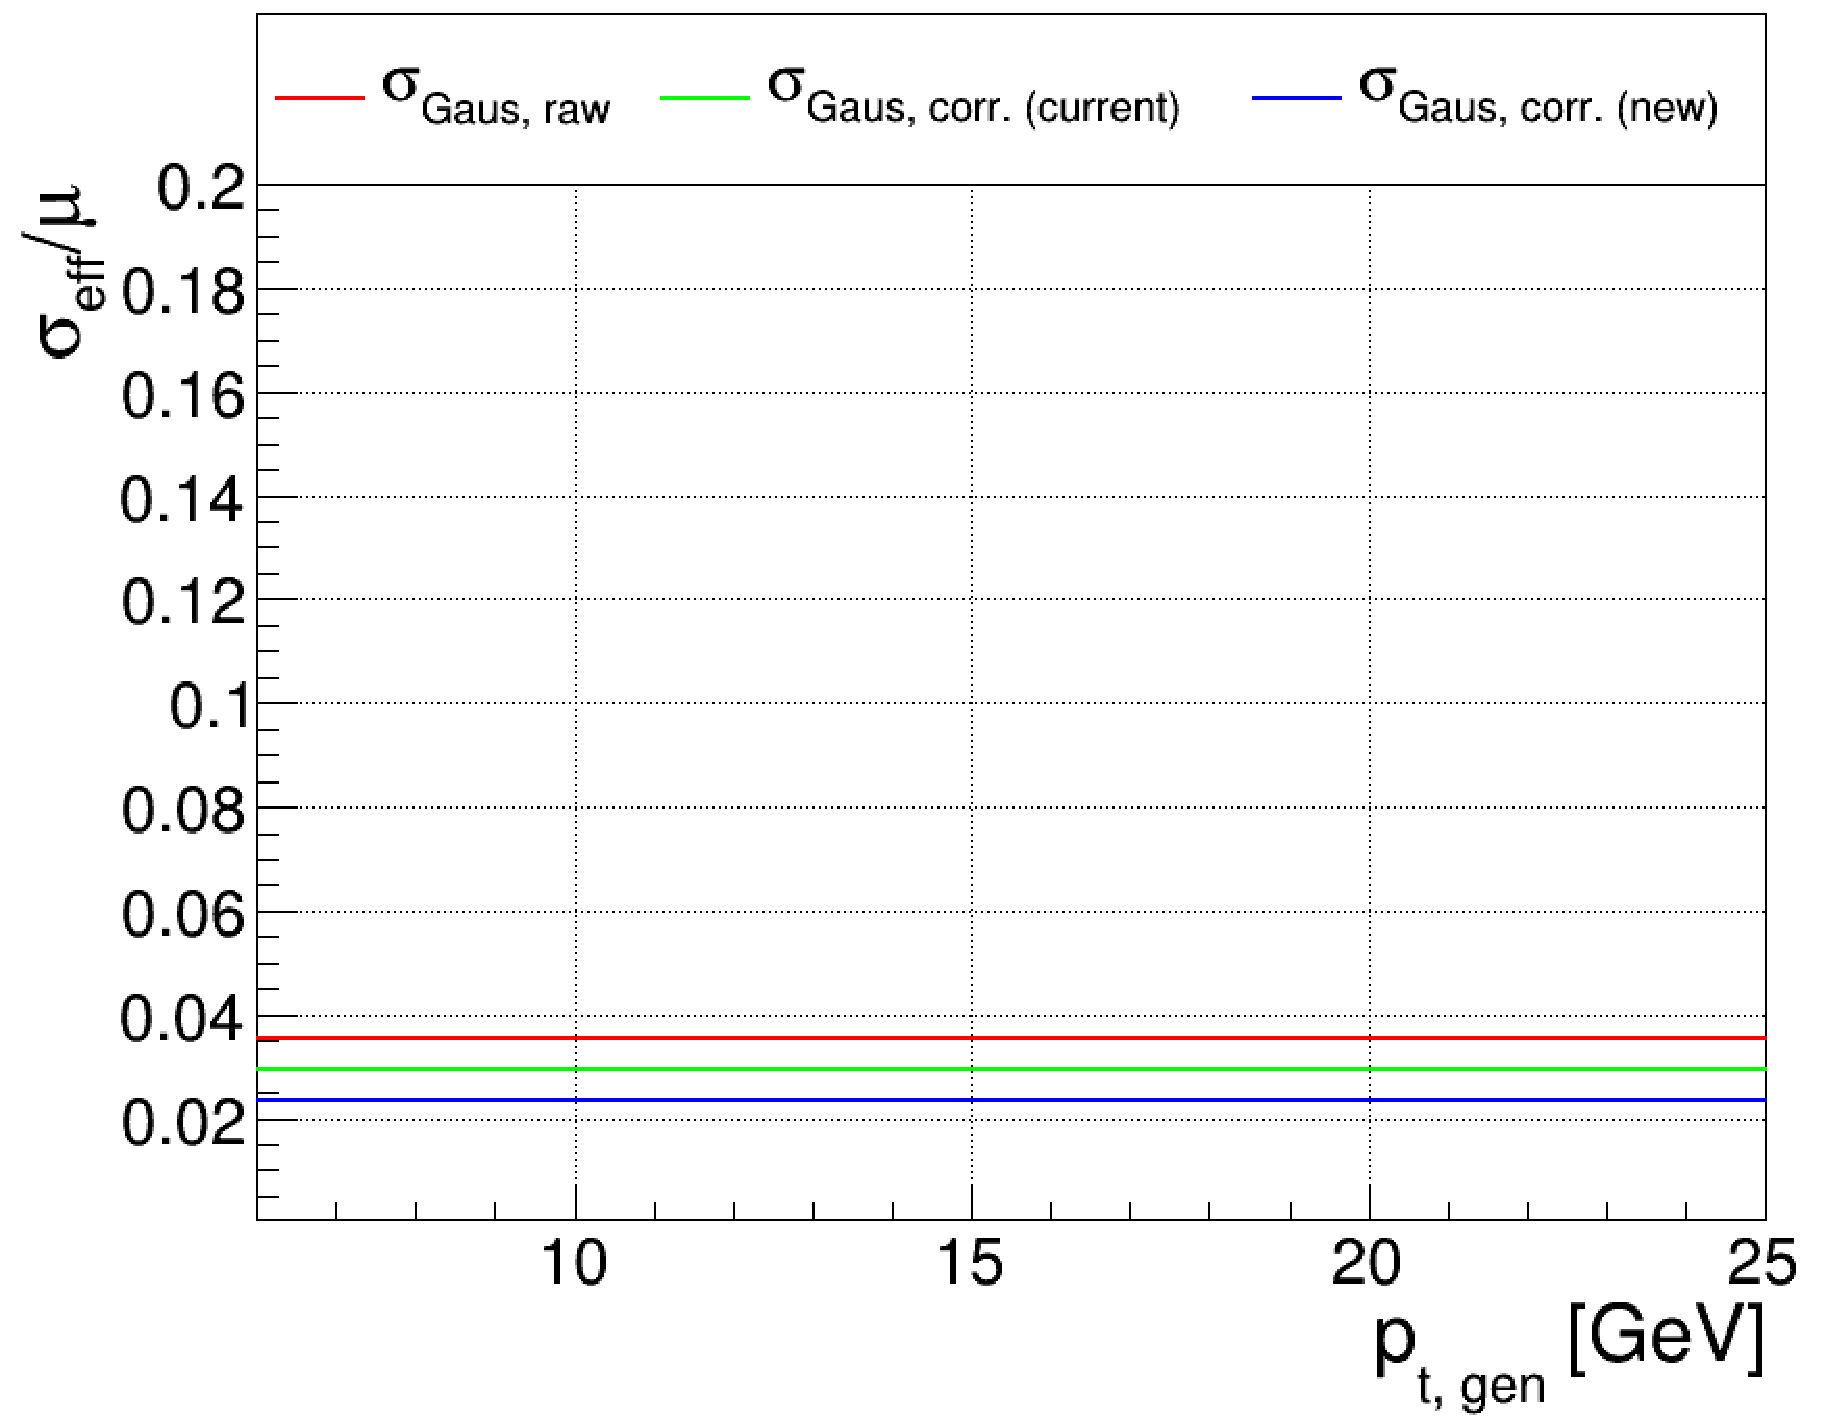
\includegraphics[width=0.495\textwidth]{./ECAL_plots/plotsNOPU/EB/ZS/pdf/GENPT/EBZS_GENPT_0006_0025_EffSigmaOverBins.pdf}
%\caption{EB - ZS Readout pt 6-25}
%\end{figure}
%\begin{figure}
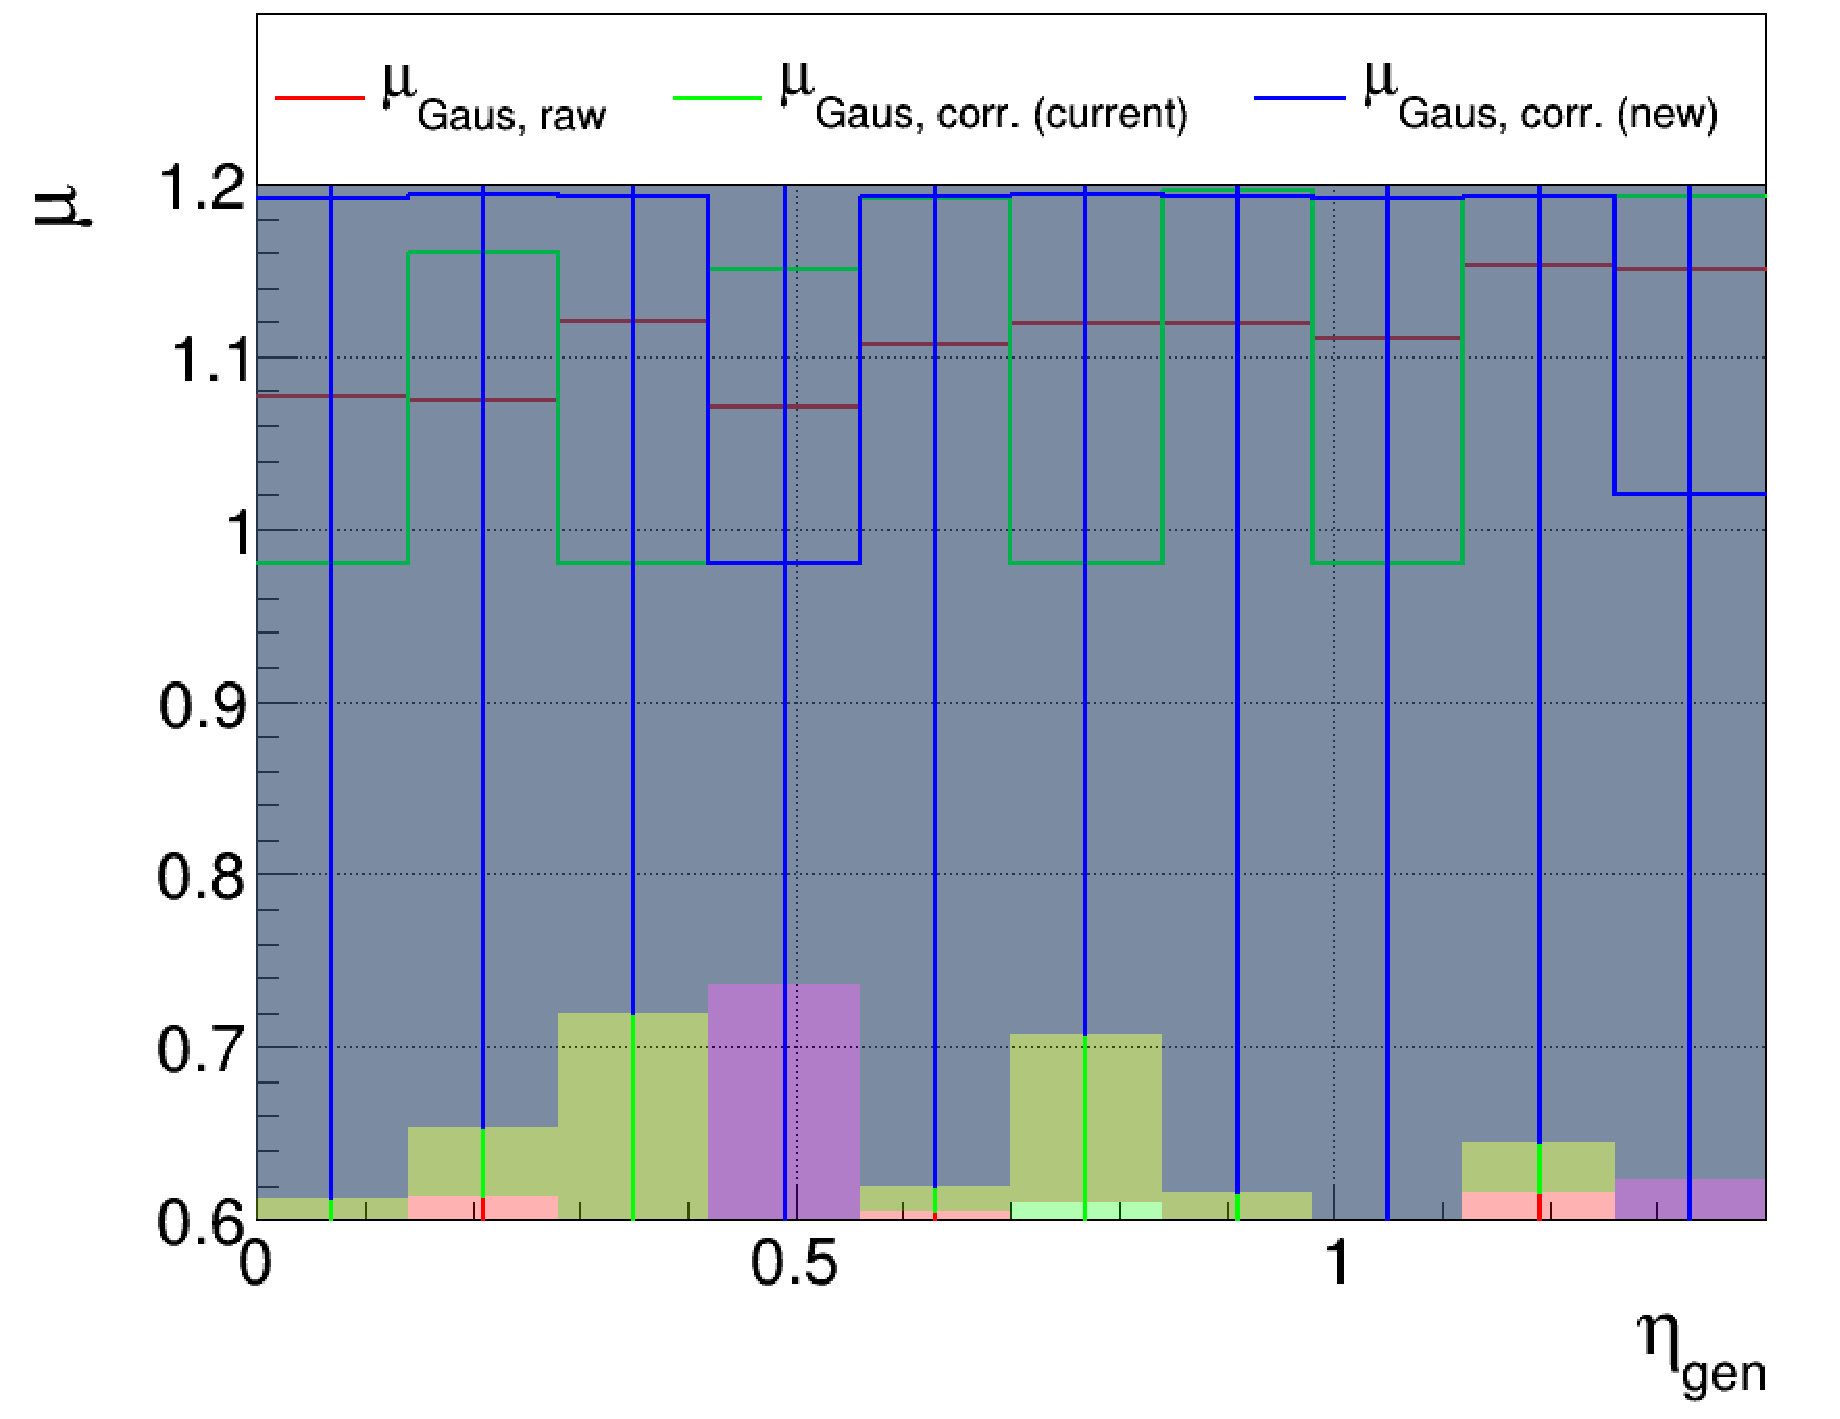
\includegraphics[width=0.495\textwidth]{./ECAL_plots/plotsNOPU/EB/ZS/pdf/GENETA/EBZS_GENETA_0006_0025_MuOverBins.pdf}
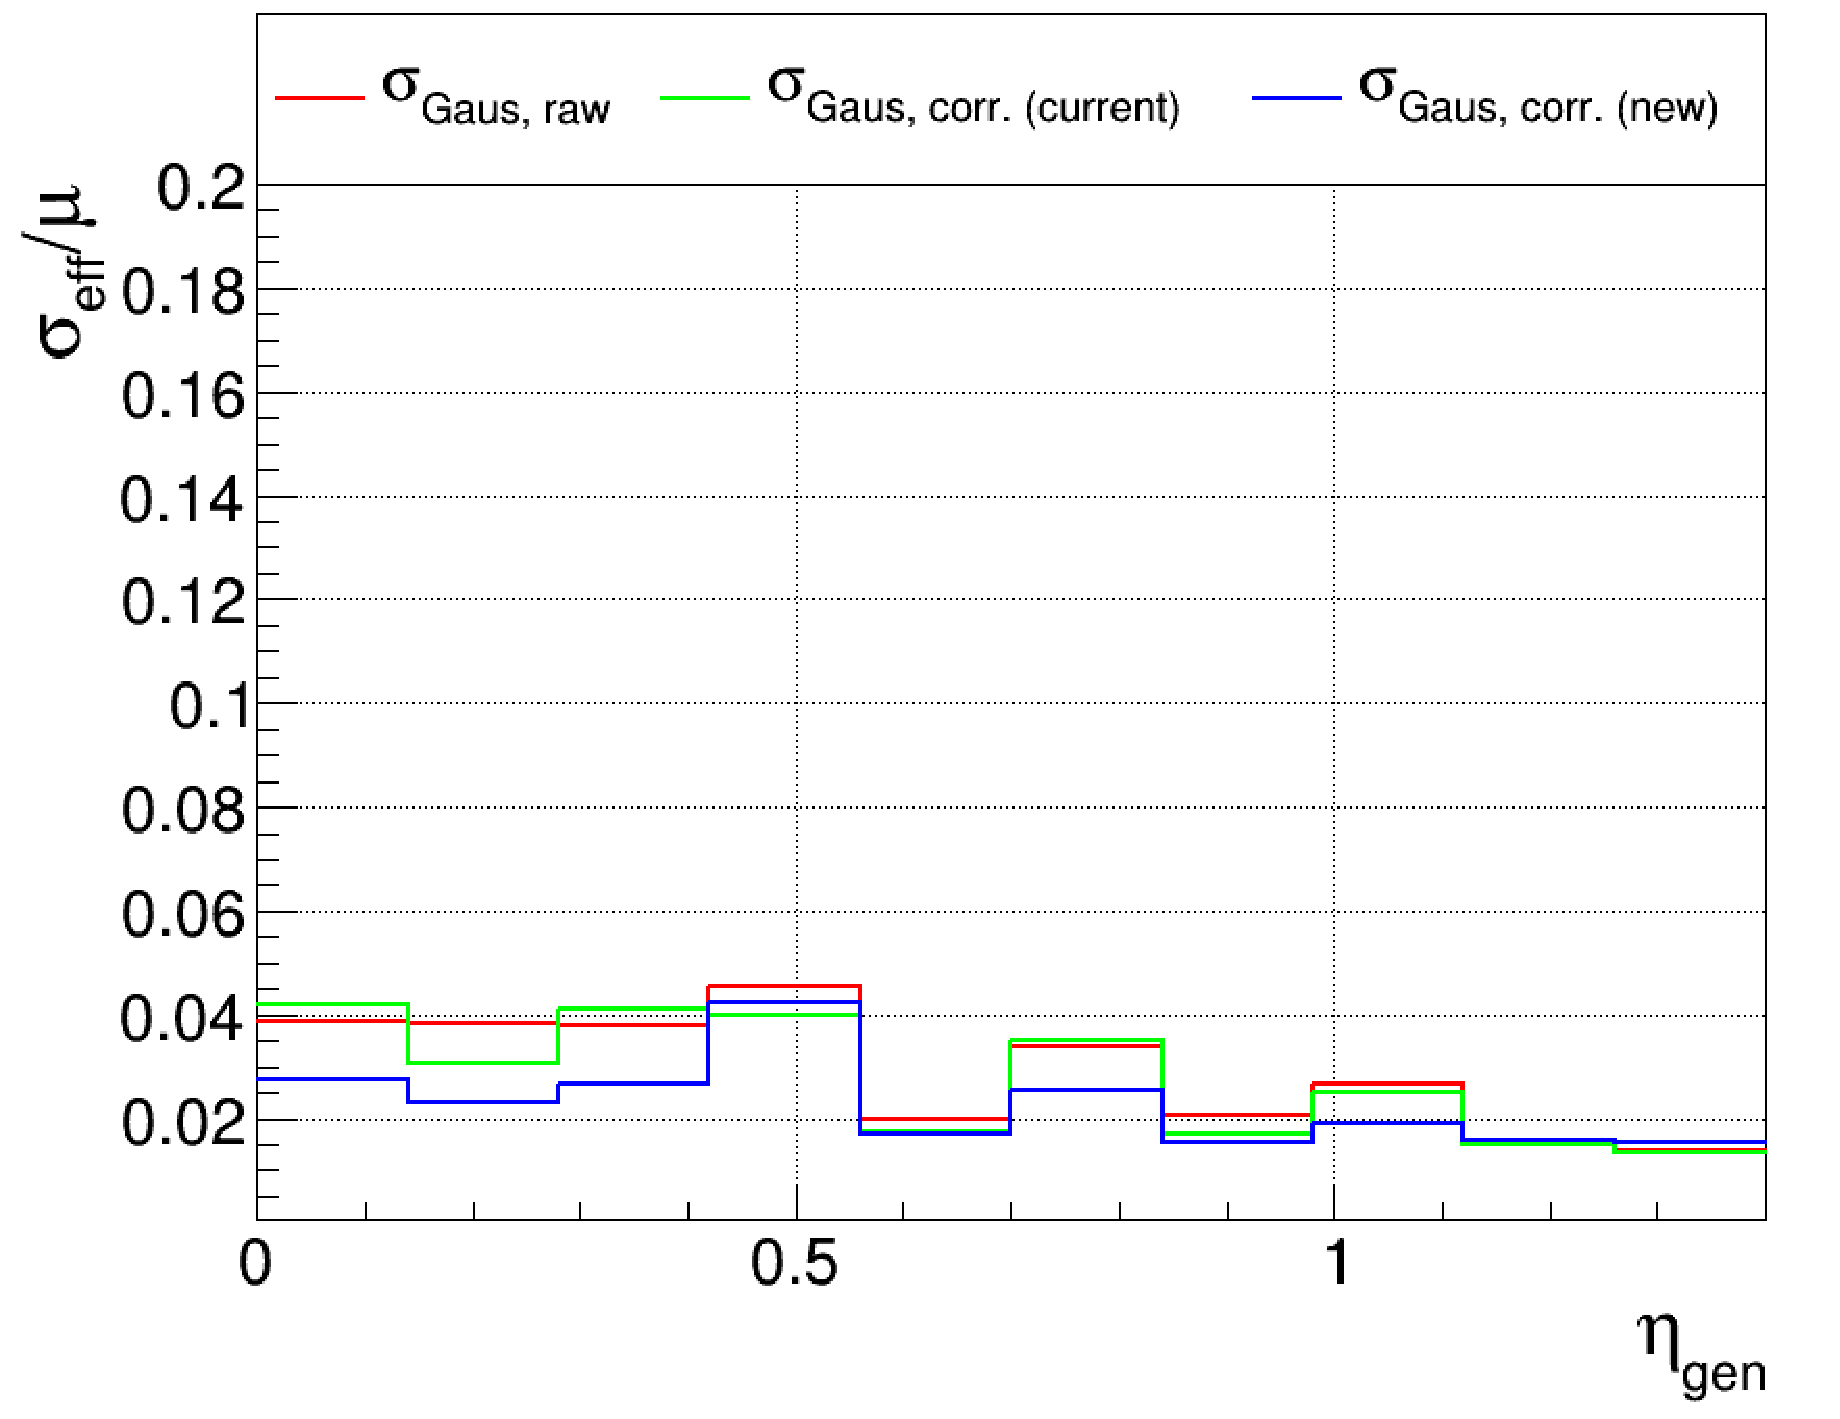
\includegraphics[width=0.495\textwidth]{./ECAL_plots/plotsNOPU/EB/ZS/pdf/GENETA/EBZS_GENETA_0006_0025_EffSigmaOverBins.pdf}
\caption{EB - ZS Readout pt 6-25}
\end{figure}






\subsection{ECAL Endcap}
in EE region:
\begin{figure}
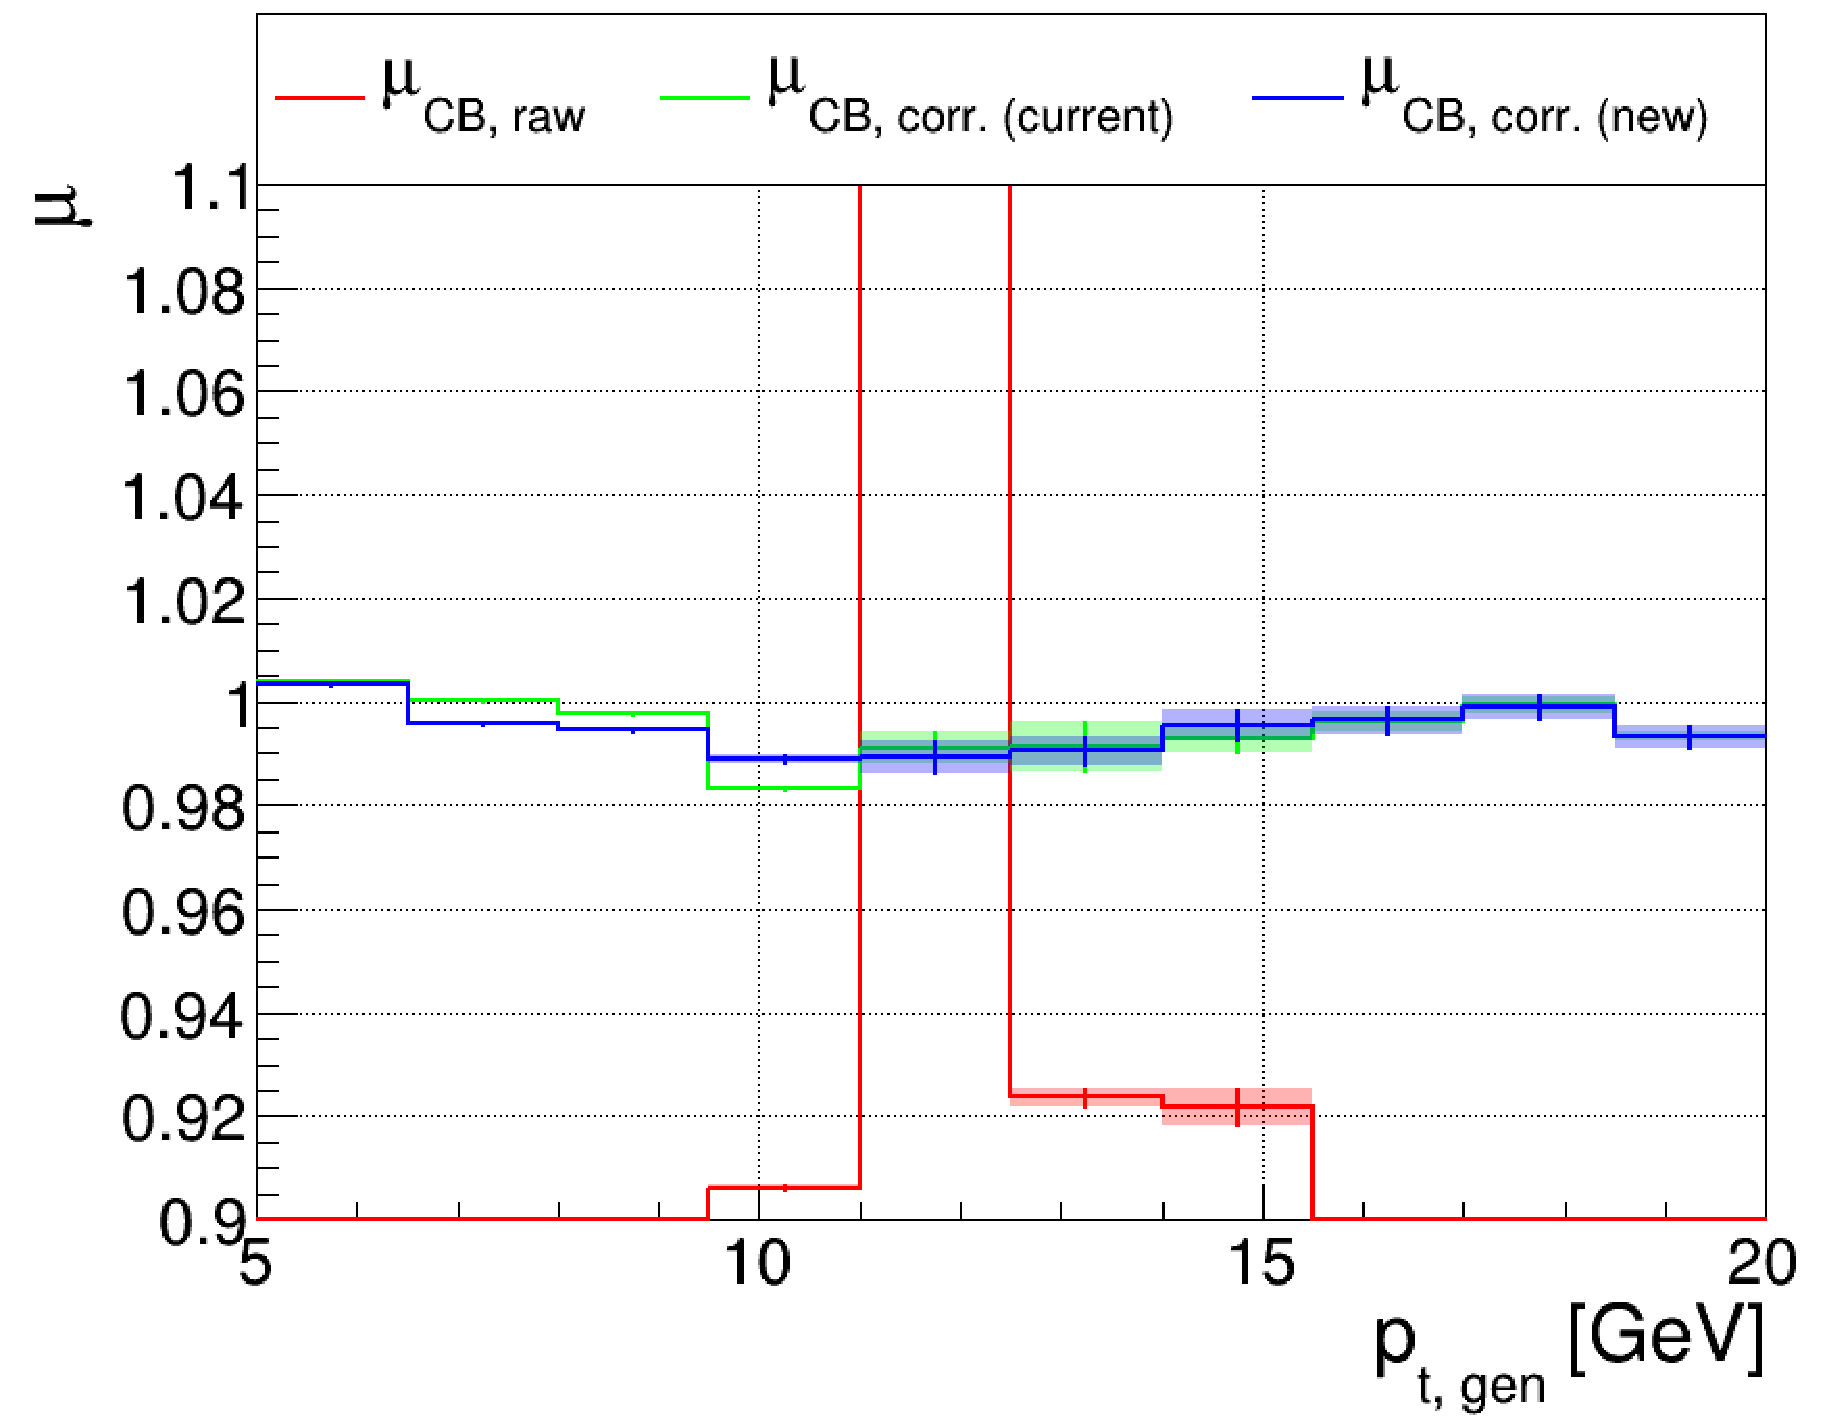
\includegraphics[width=0.495\textwidth]{./ECAL_plots/plotsNoPU/EE/pdf/FULL/GENPT/EEFULL_GENPT_0005_0020_MuOverBins.pdf}
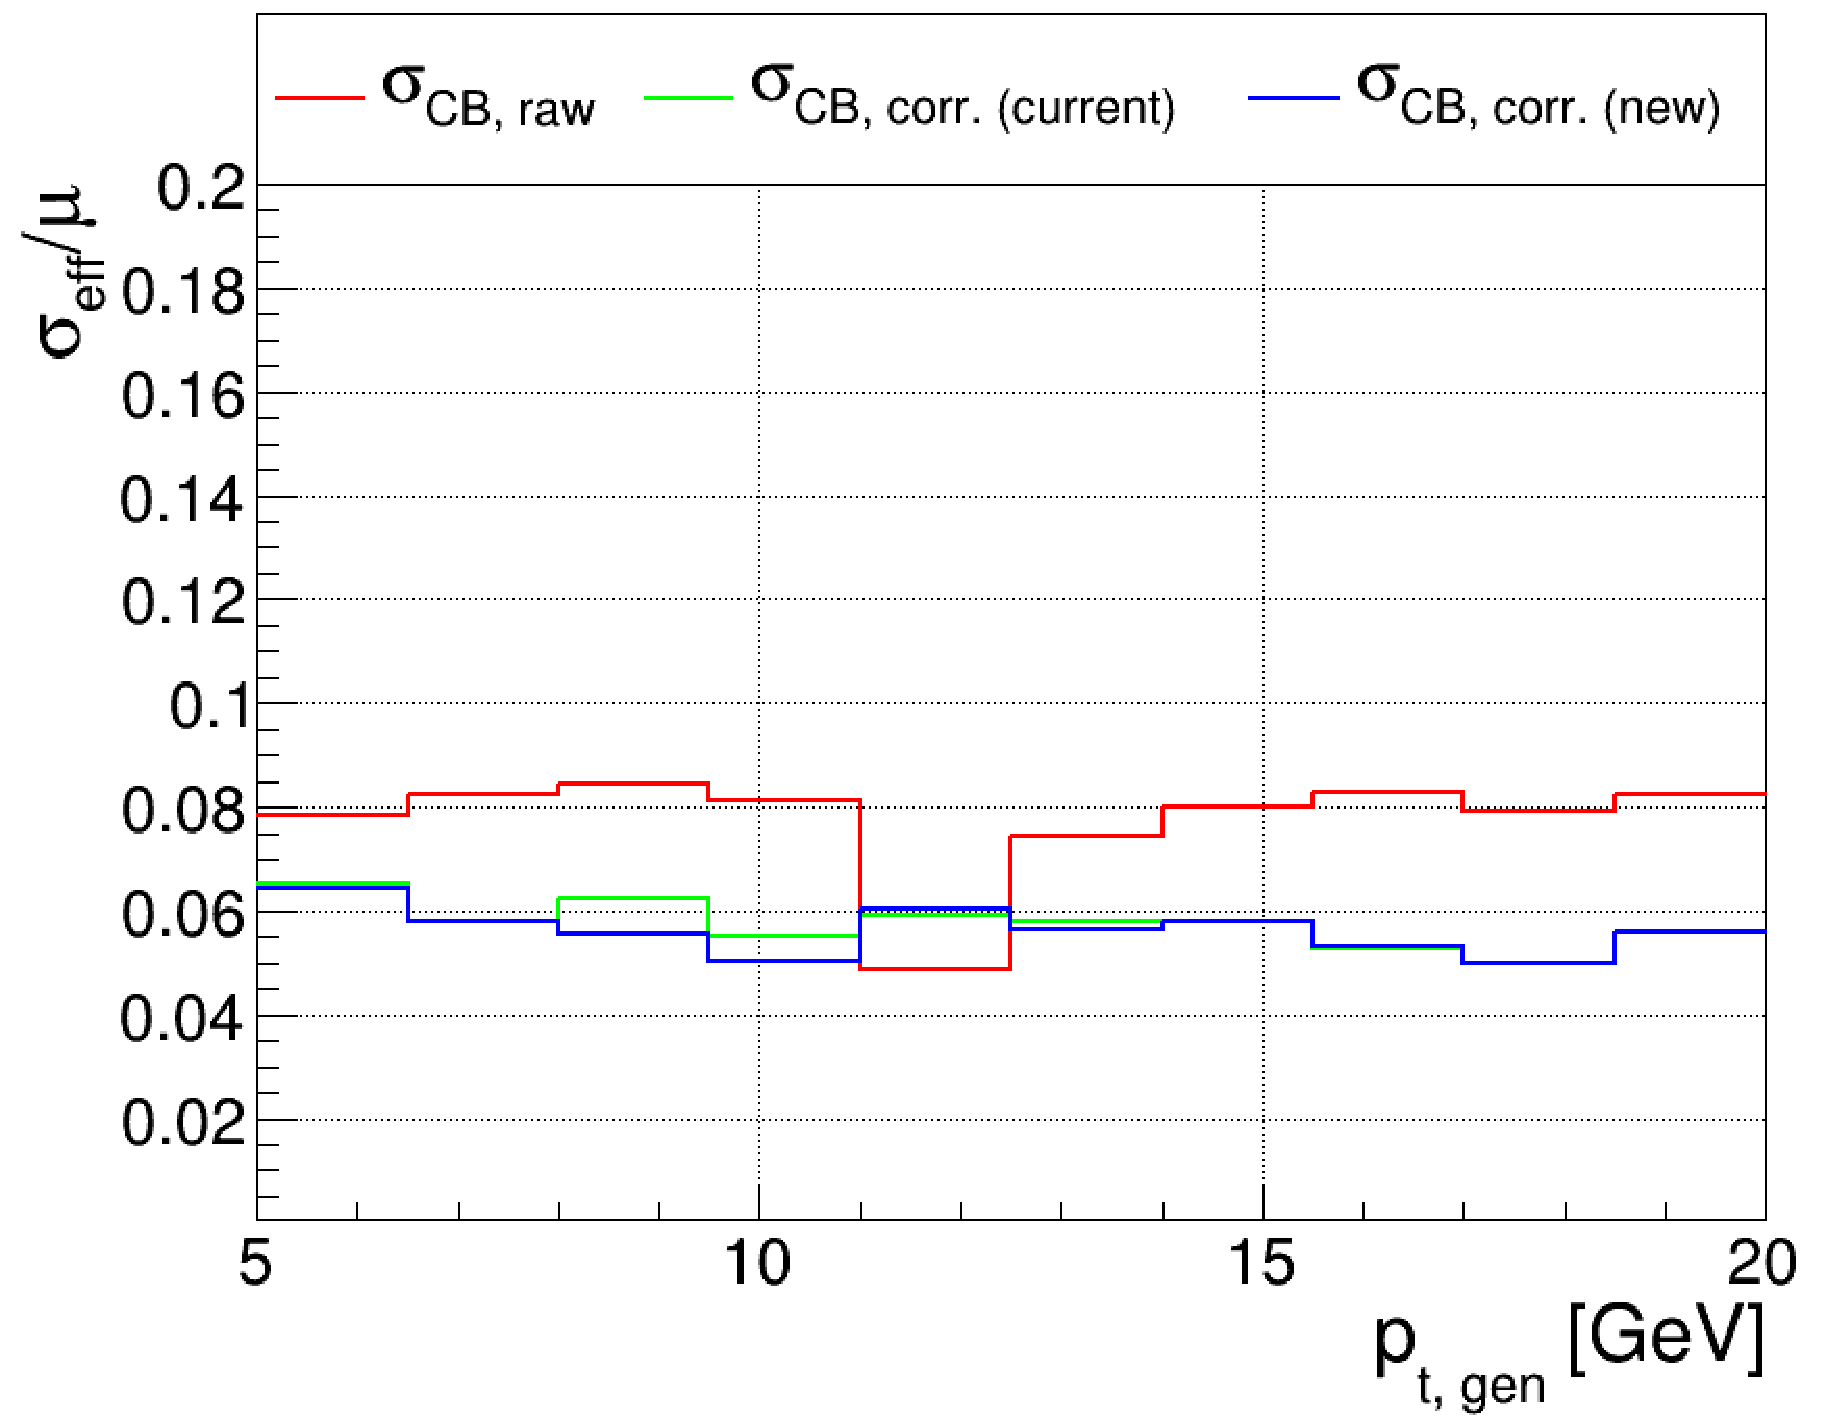
\includegraphics[width=0.495\textwidth]{./ECAL_plots/plotsNoPU/EE/pdf/FULL/GENPT/EEFULL_GENPT_0005_0020_EffSigmaOverBins.pdf}
%\caption{EE - Full Readout pt 5-20}
%\end{figure}
%\begin{figure}
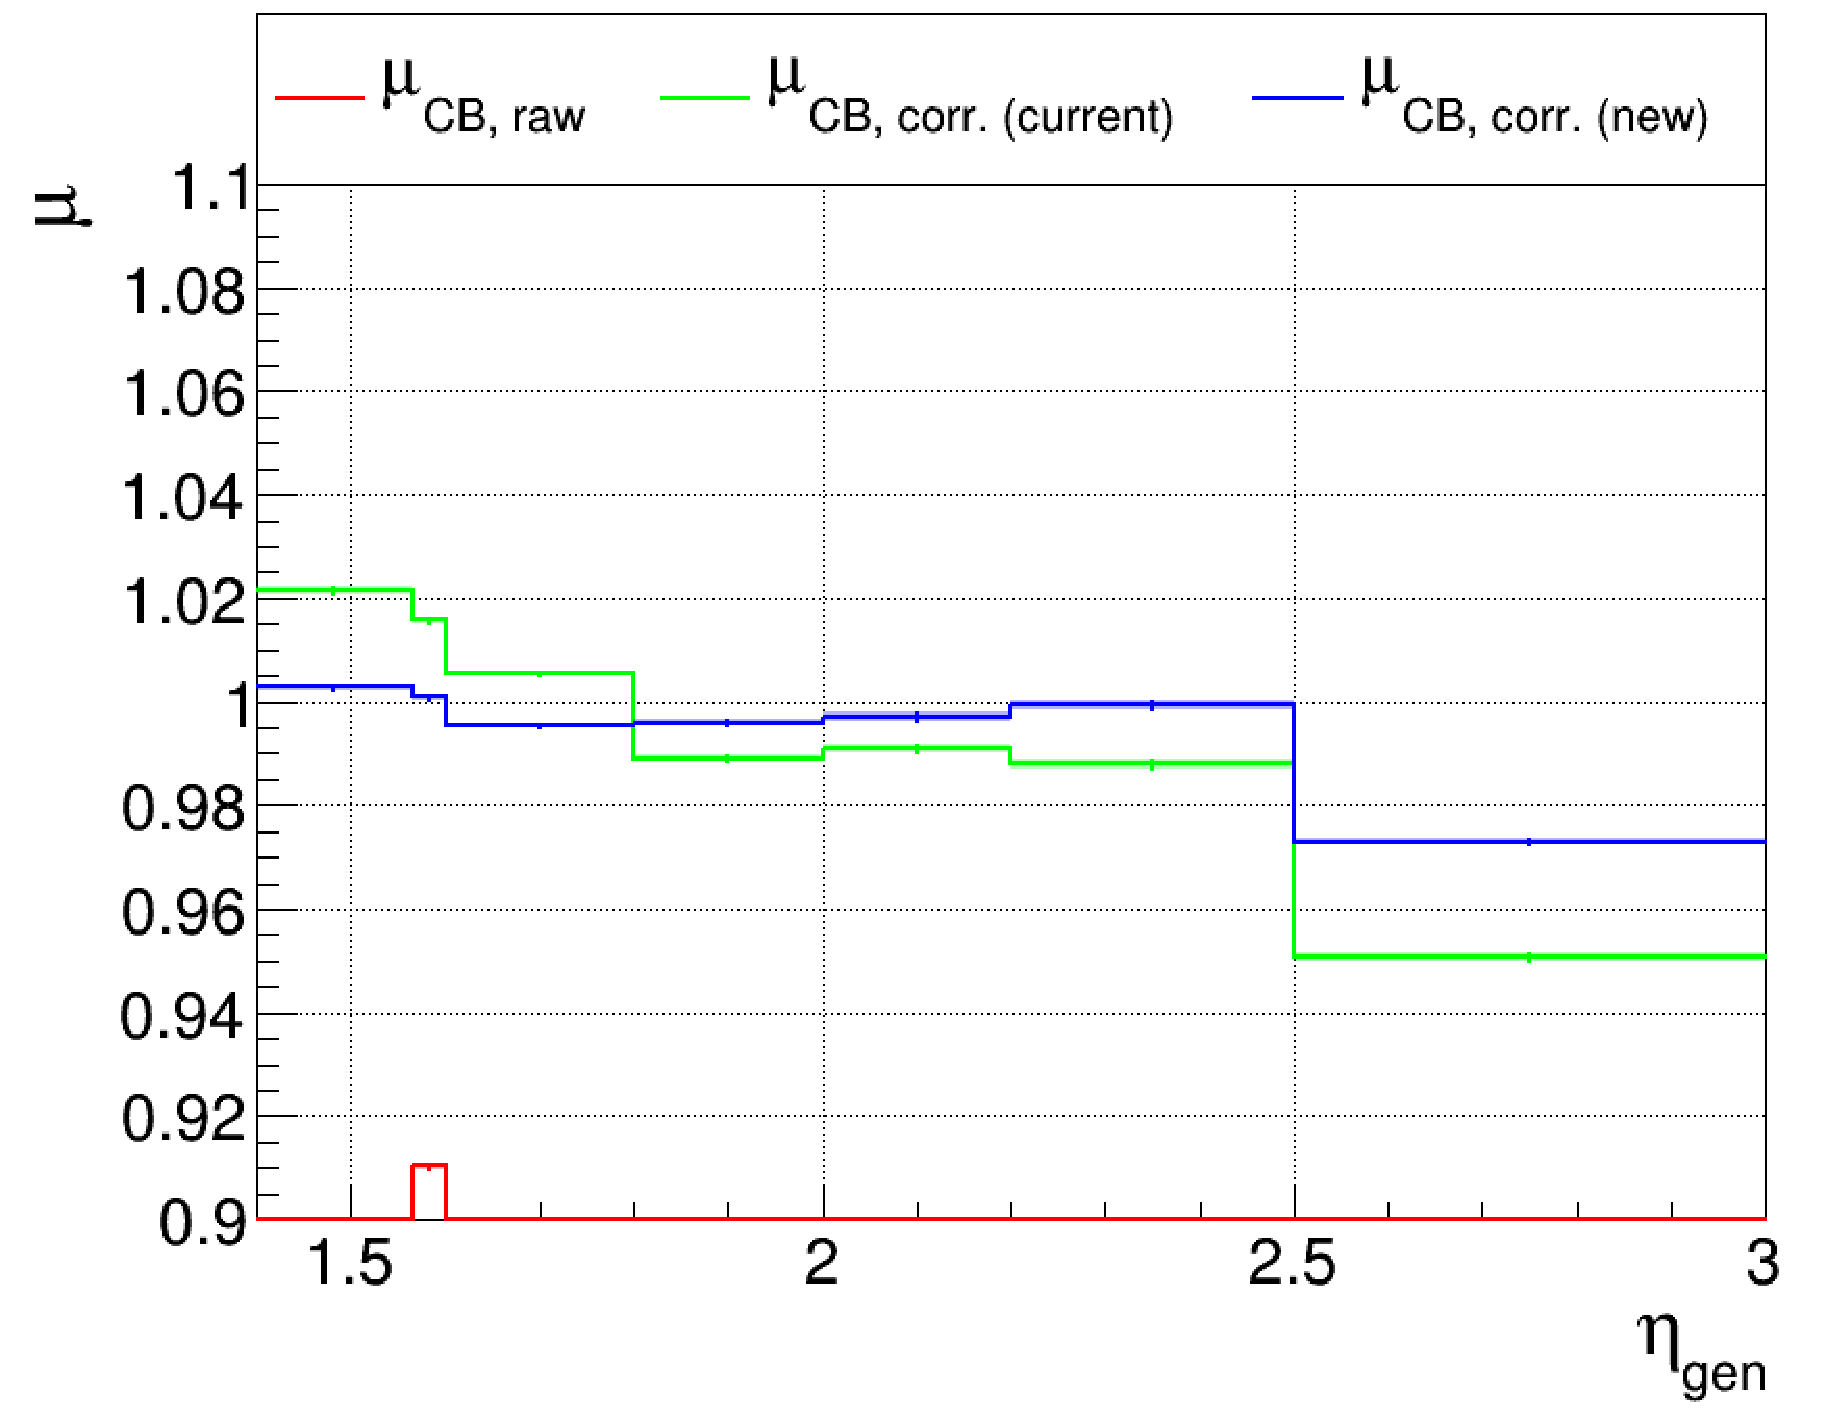
\includegraphics[width=0.495\textwidth]{./ECAL_plots/plotsNoPU/EE/pdf/FULL/GENETA/EEFULL_GENETA_0005_0020_MuOverBins.pdf}
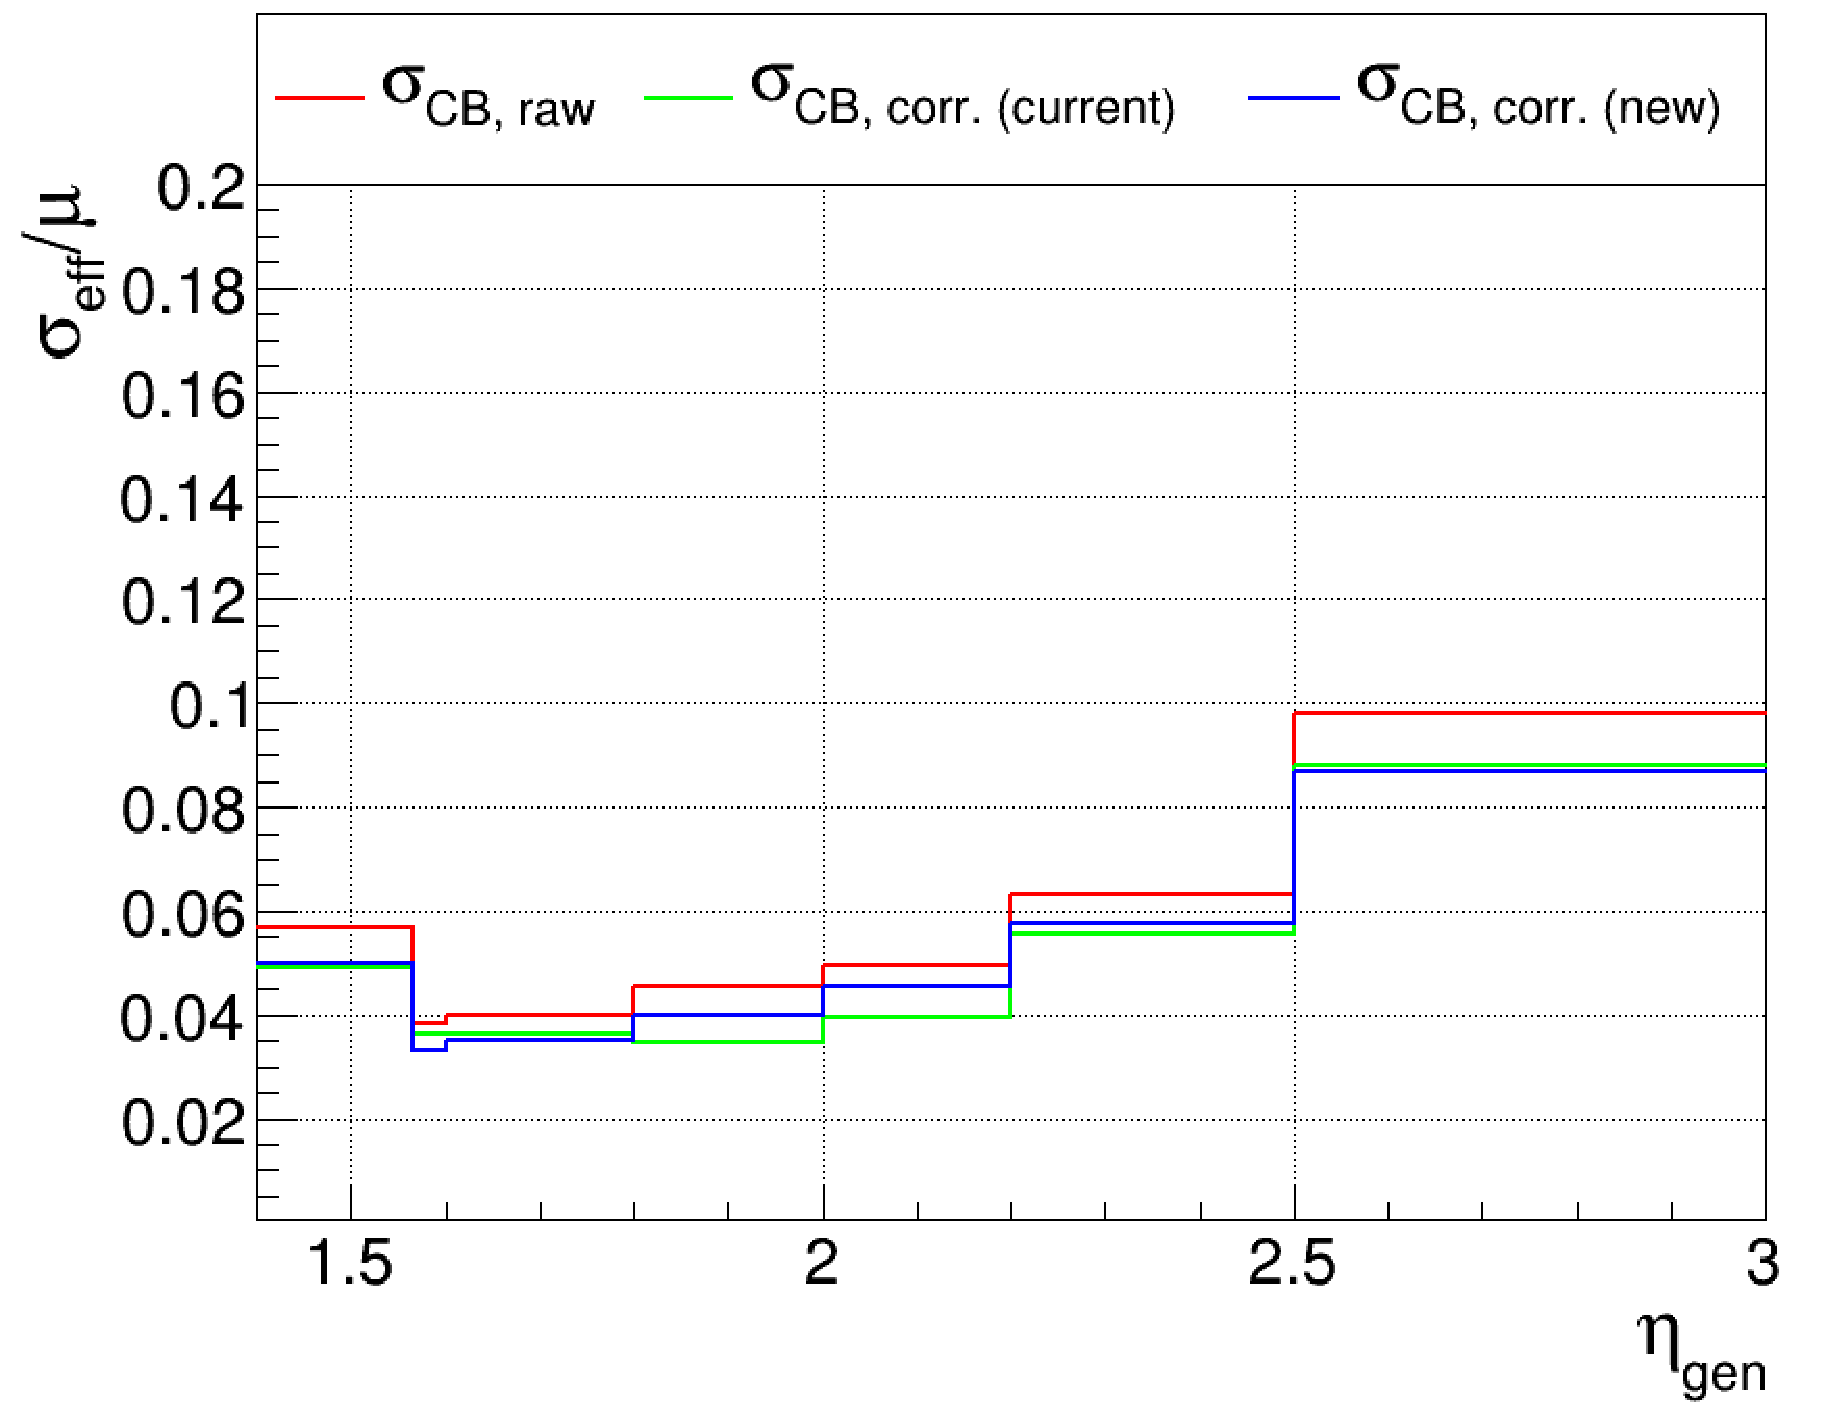
\includegraphics[width=0.495\textwidth]{./ECAL_plots/plotsNoPU/EE/pdf/FULL/GENETA/EEFULL_GENETA_0005_0020_EffSigmaOverBins.pdf}
\caption{EE - Full Readout pt 5-20}
\end{figure}


\begin{figure}
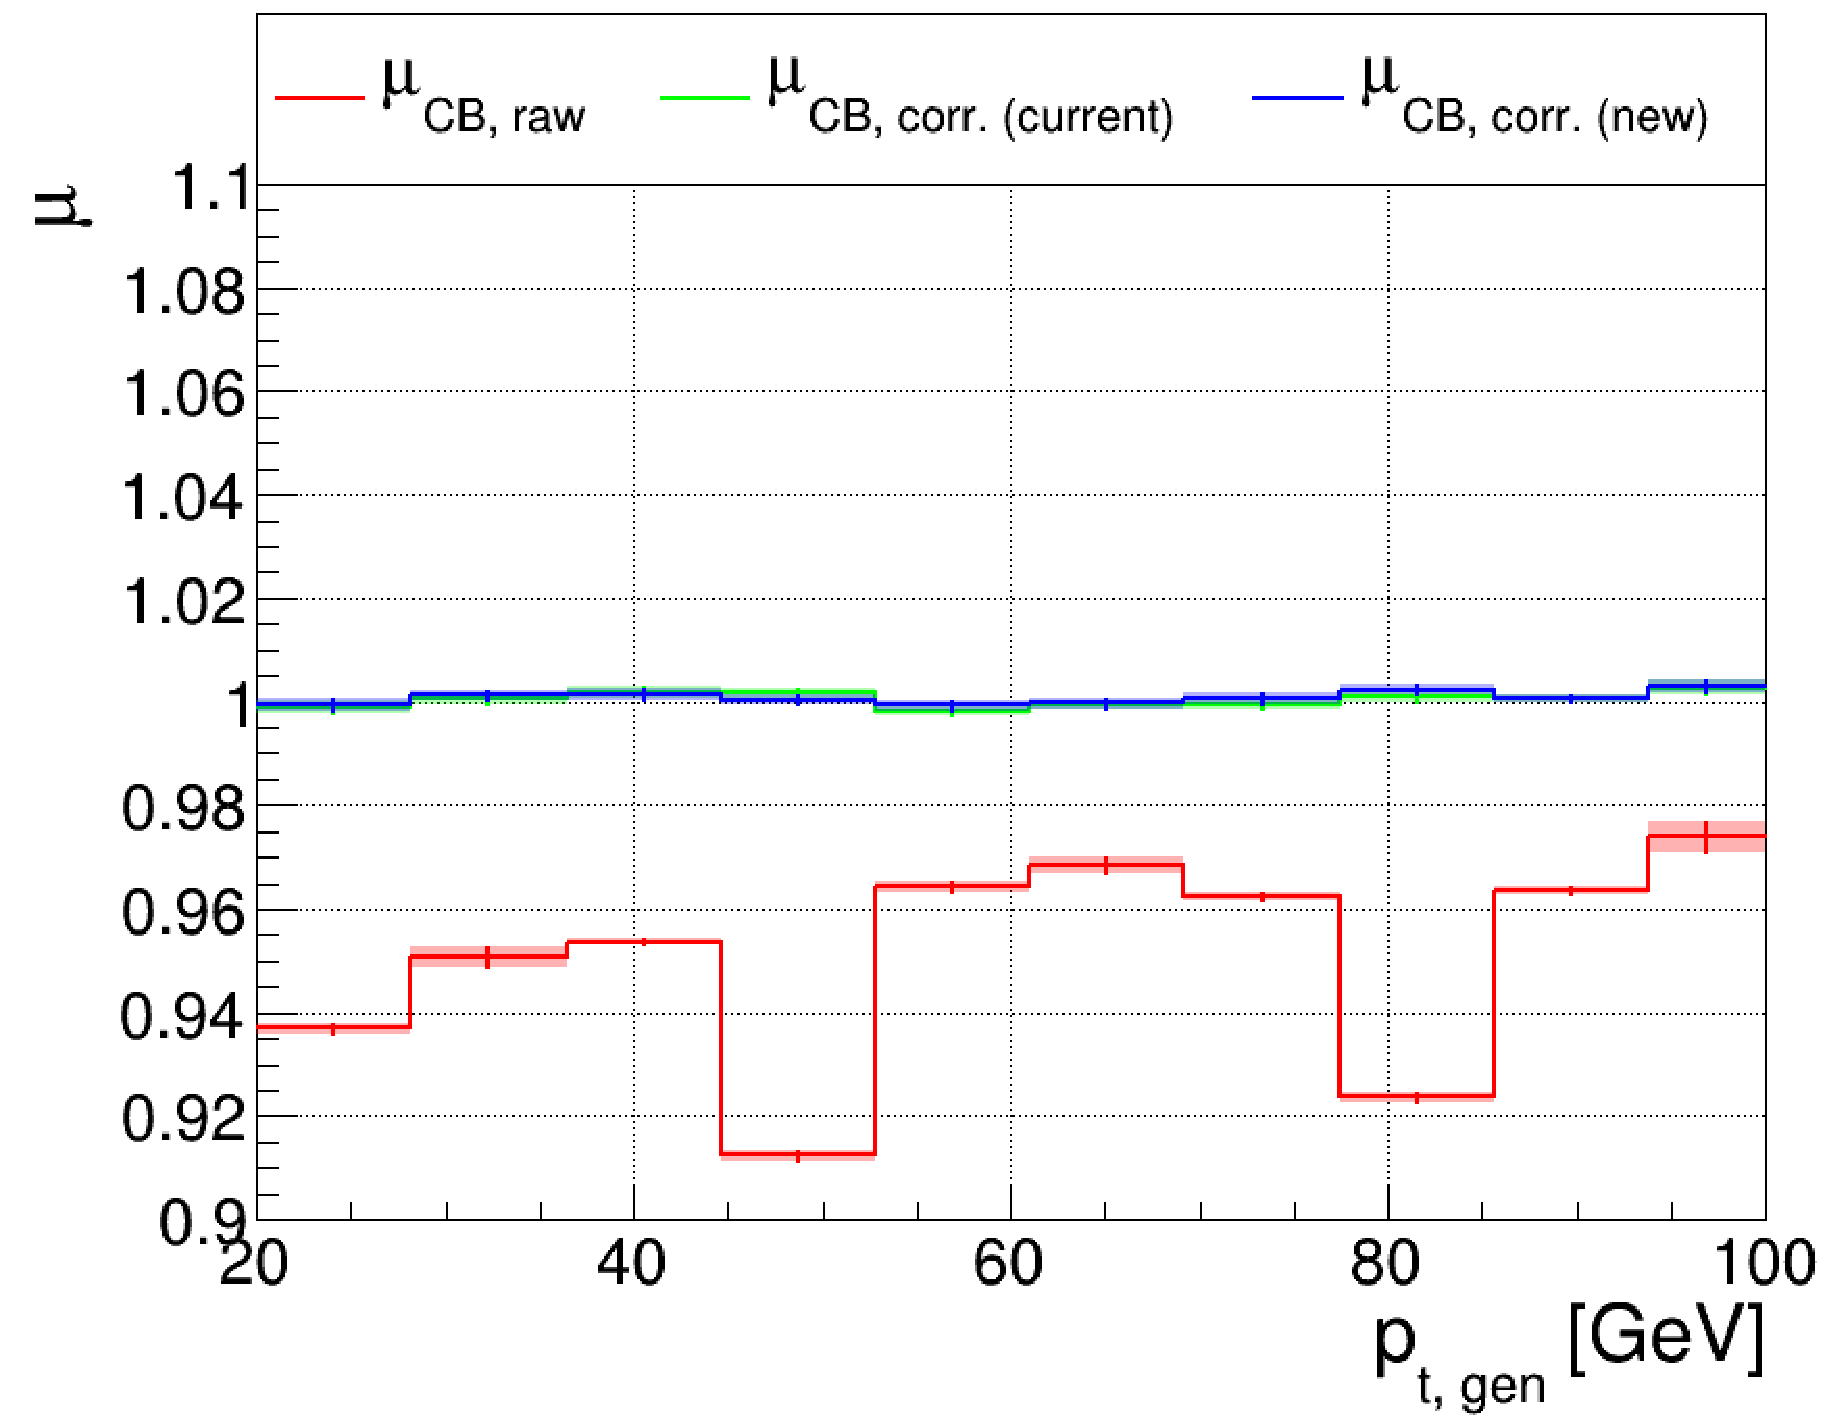
\includegraphics[width=0.495\textwidth]{./ECAL_plots/plotsNoPU/EE/pdf/FULL/GENPT/EEFULL_GENPT_0020_0100_MuOverBins.pdf}
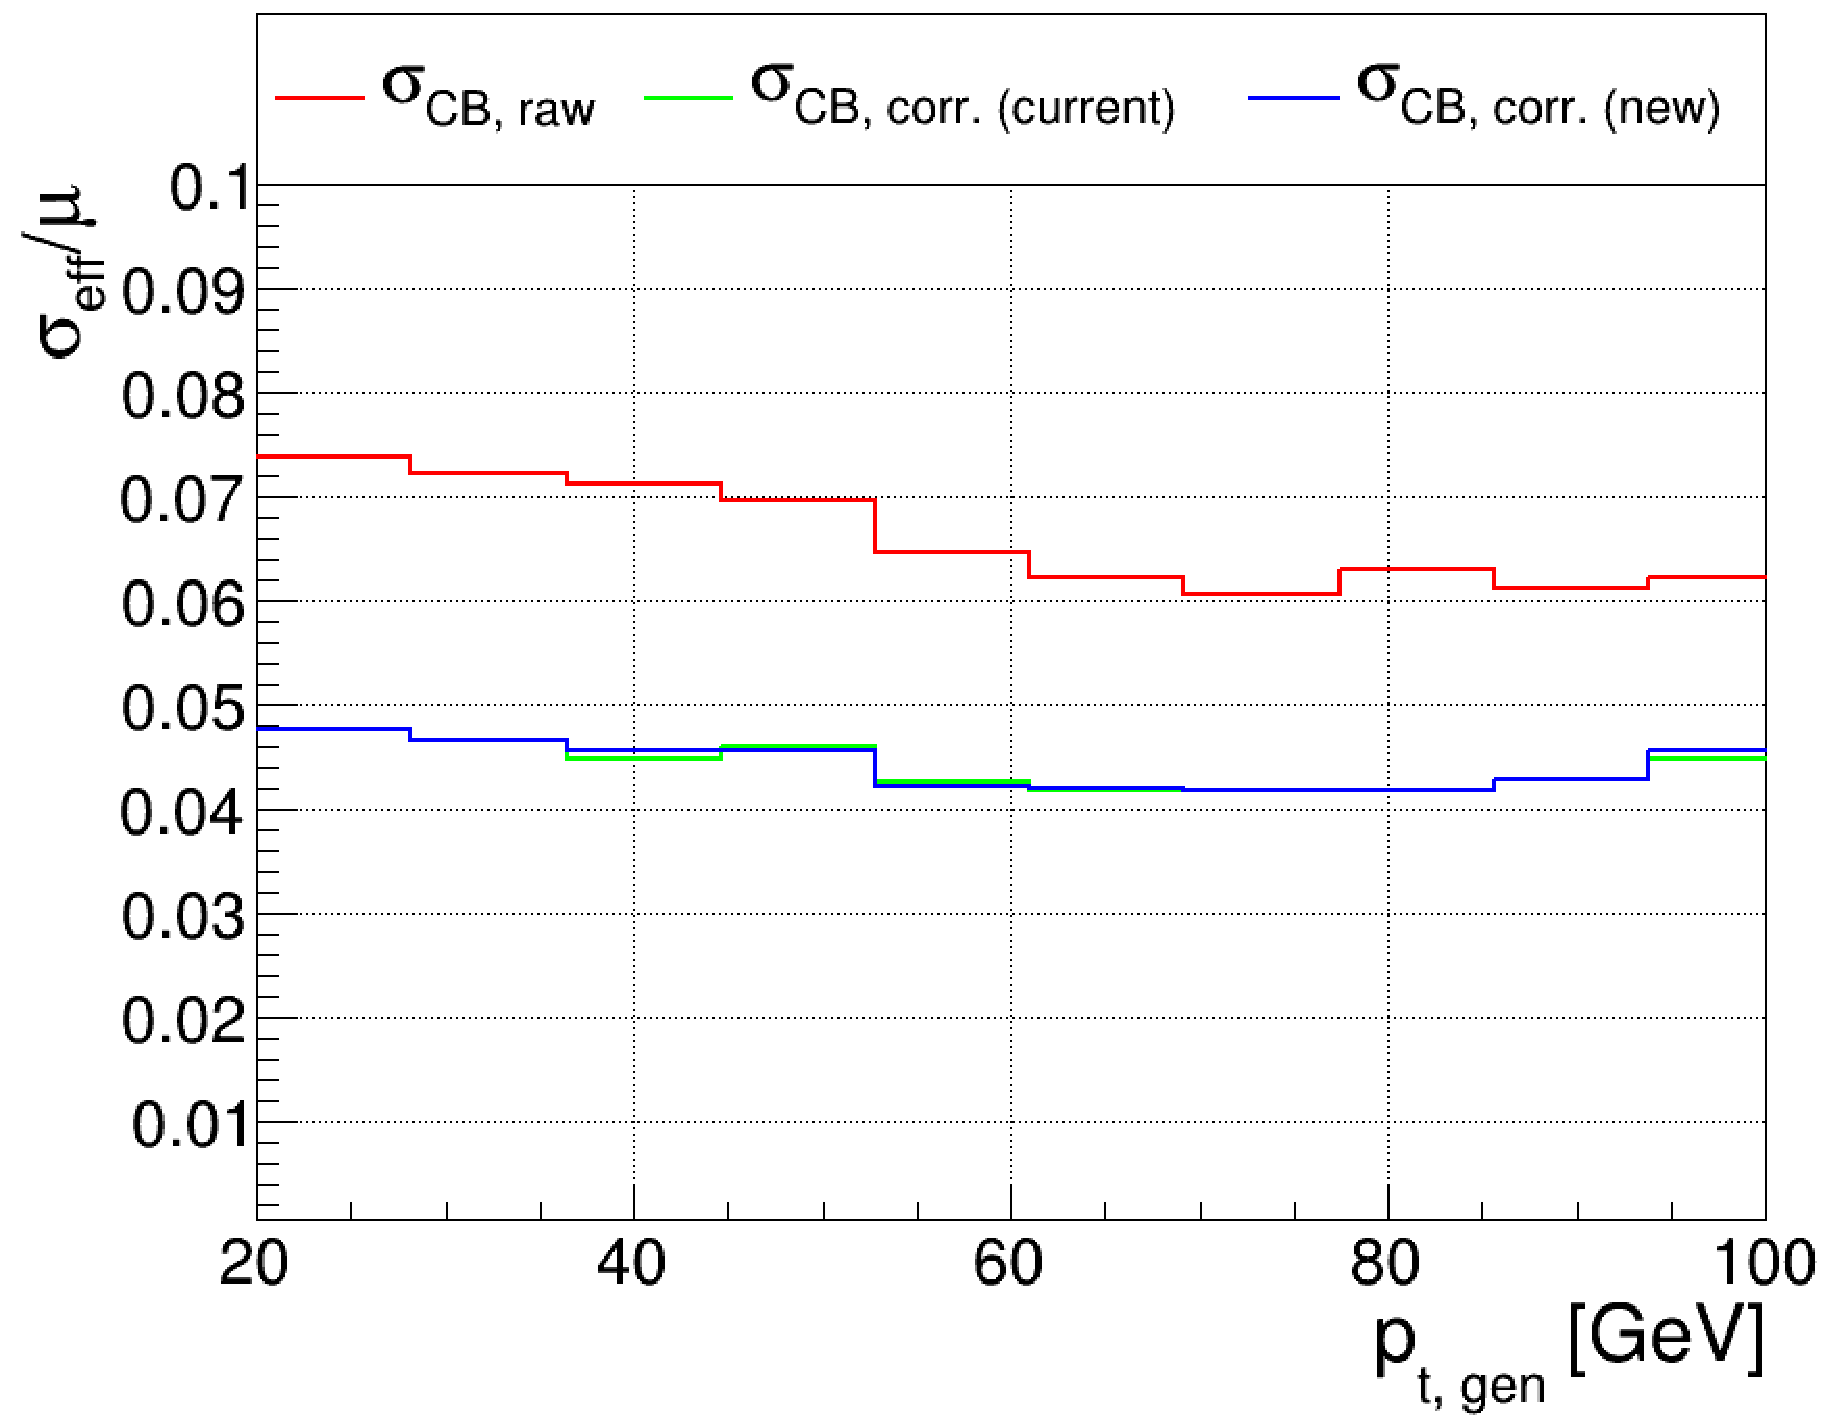
\includegraphics[width=0.495\textwidth]{./ECAL_plots/plotsNoPU/EE/pdf/FULL/GENPT/EEFULL_GENPT_0020_0100_EffSigmaOverBins.pdf}
%\caption{EE - Full Readout pt 20-100}
%\end{figure}
%\begin{figure}
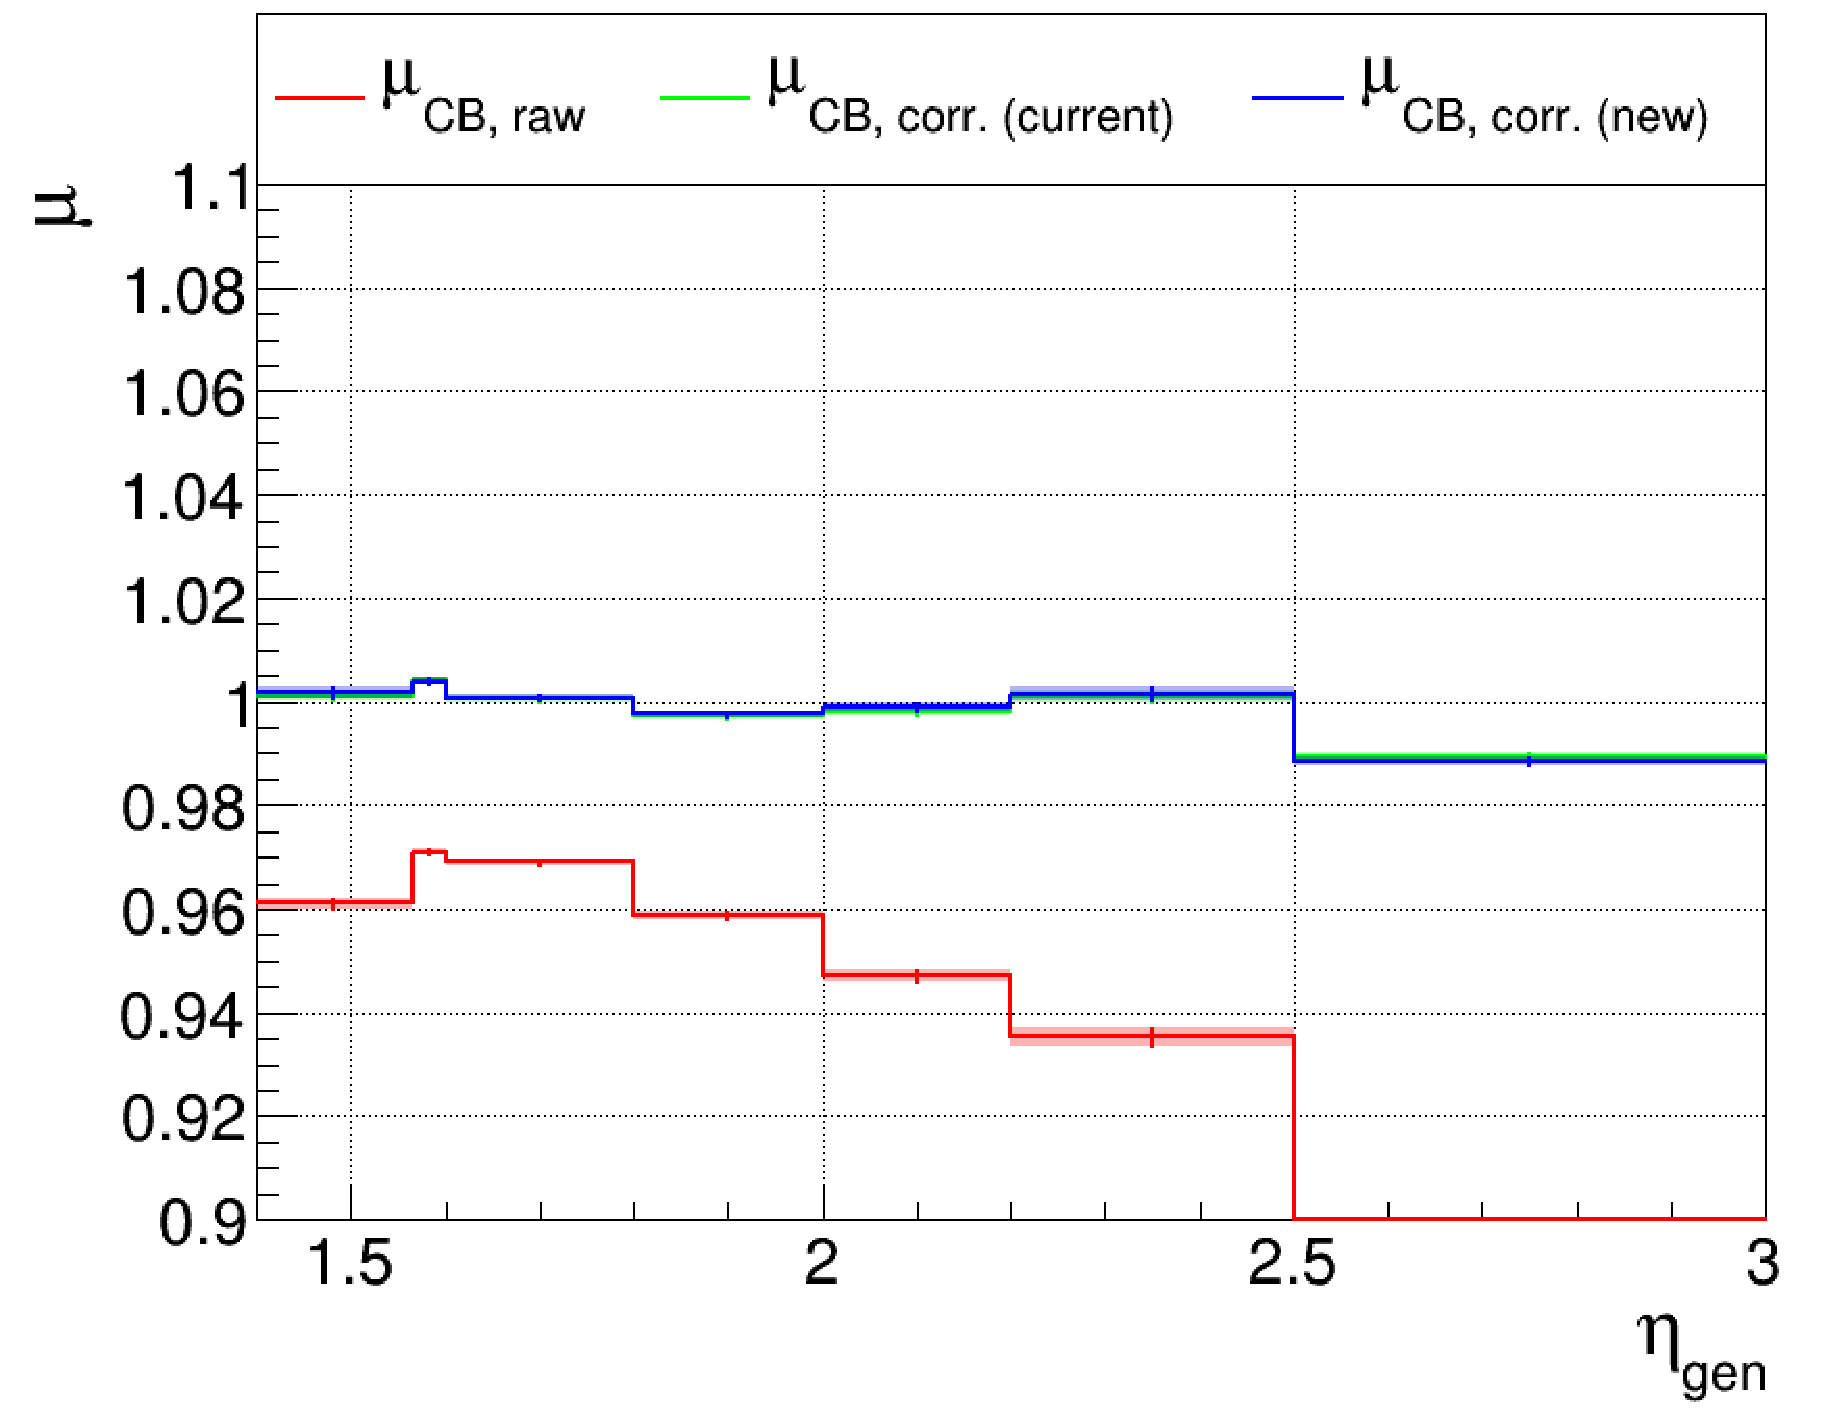
\includegraphics[width=0.495\textwidth]{./ECAL_plots/plotsNoPU/EE/pdf/FULL/GENETA/EEFULL_GENETA_0020_0100_MuOverBins.pdf}
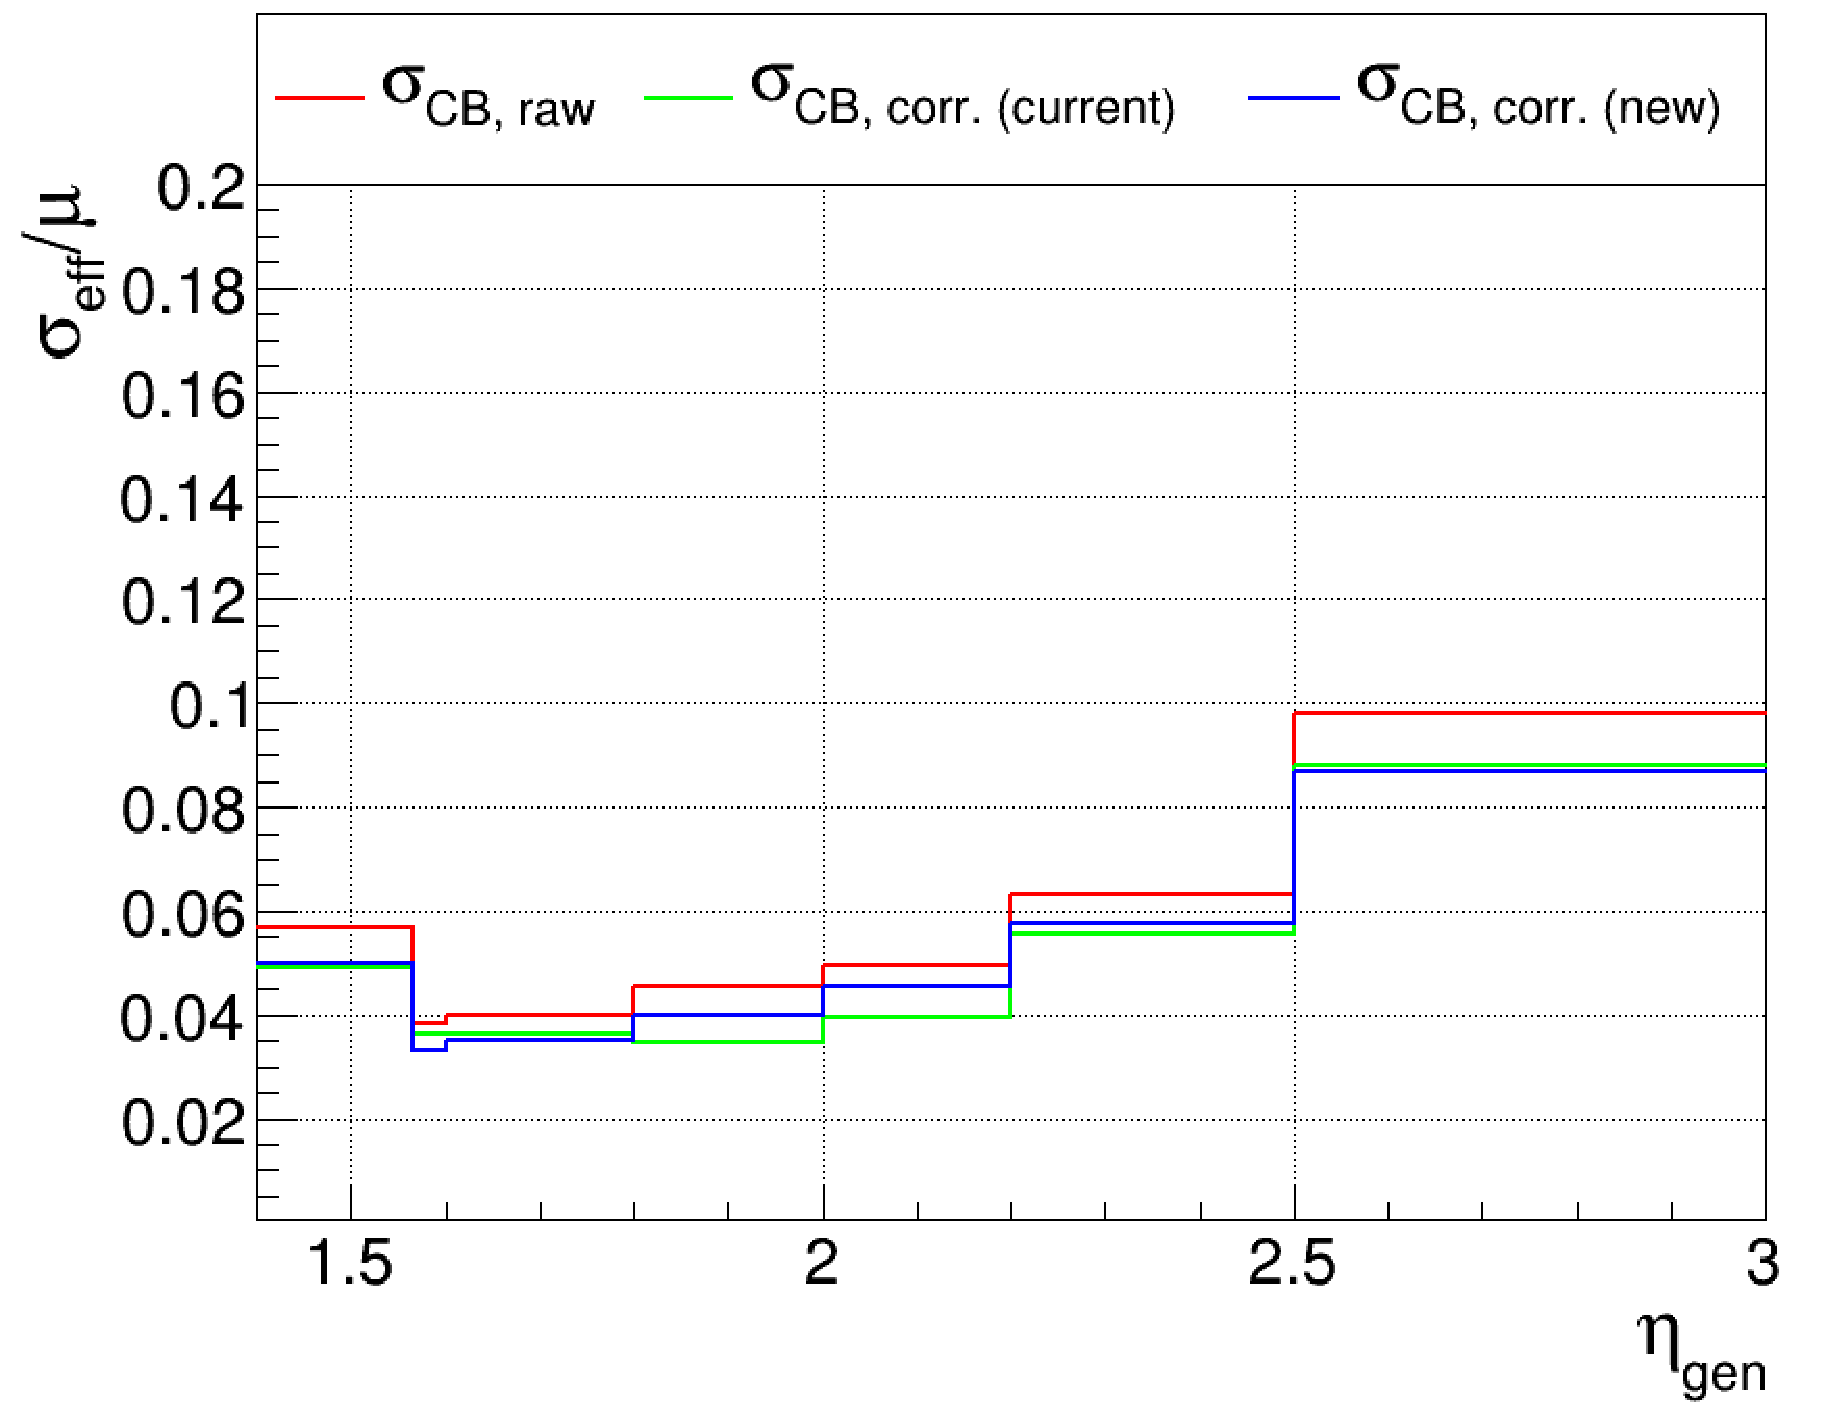
\includegraphics[width=0.495\textwidth]{./ECAL_plots/plotsNoPU/EE/pdf/FULL/GENETA/EEFULL_GENETA_0005_0020_EffSigmaOverBins.pdf}
\caption{EE - Full Readout pt 20-100}
\end{figure}


\begin{figure}
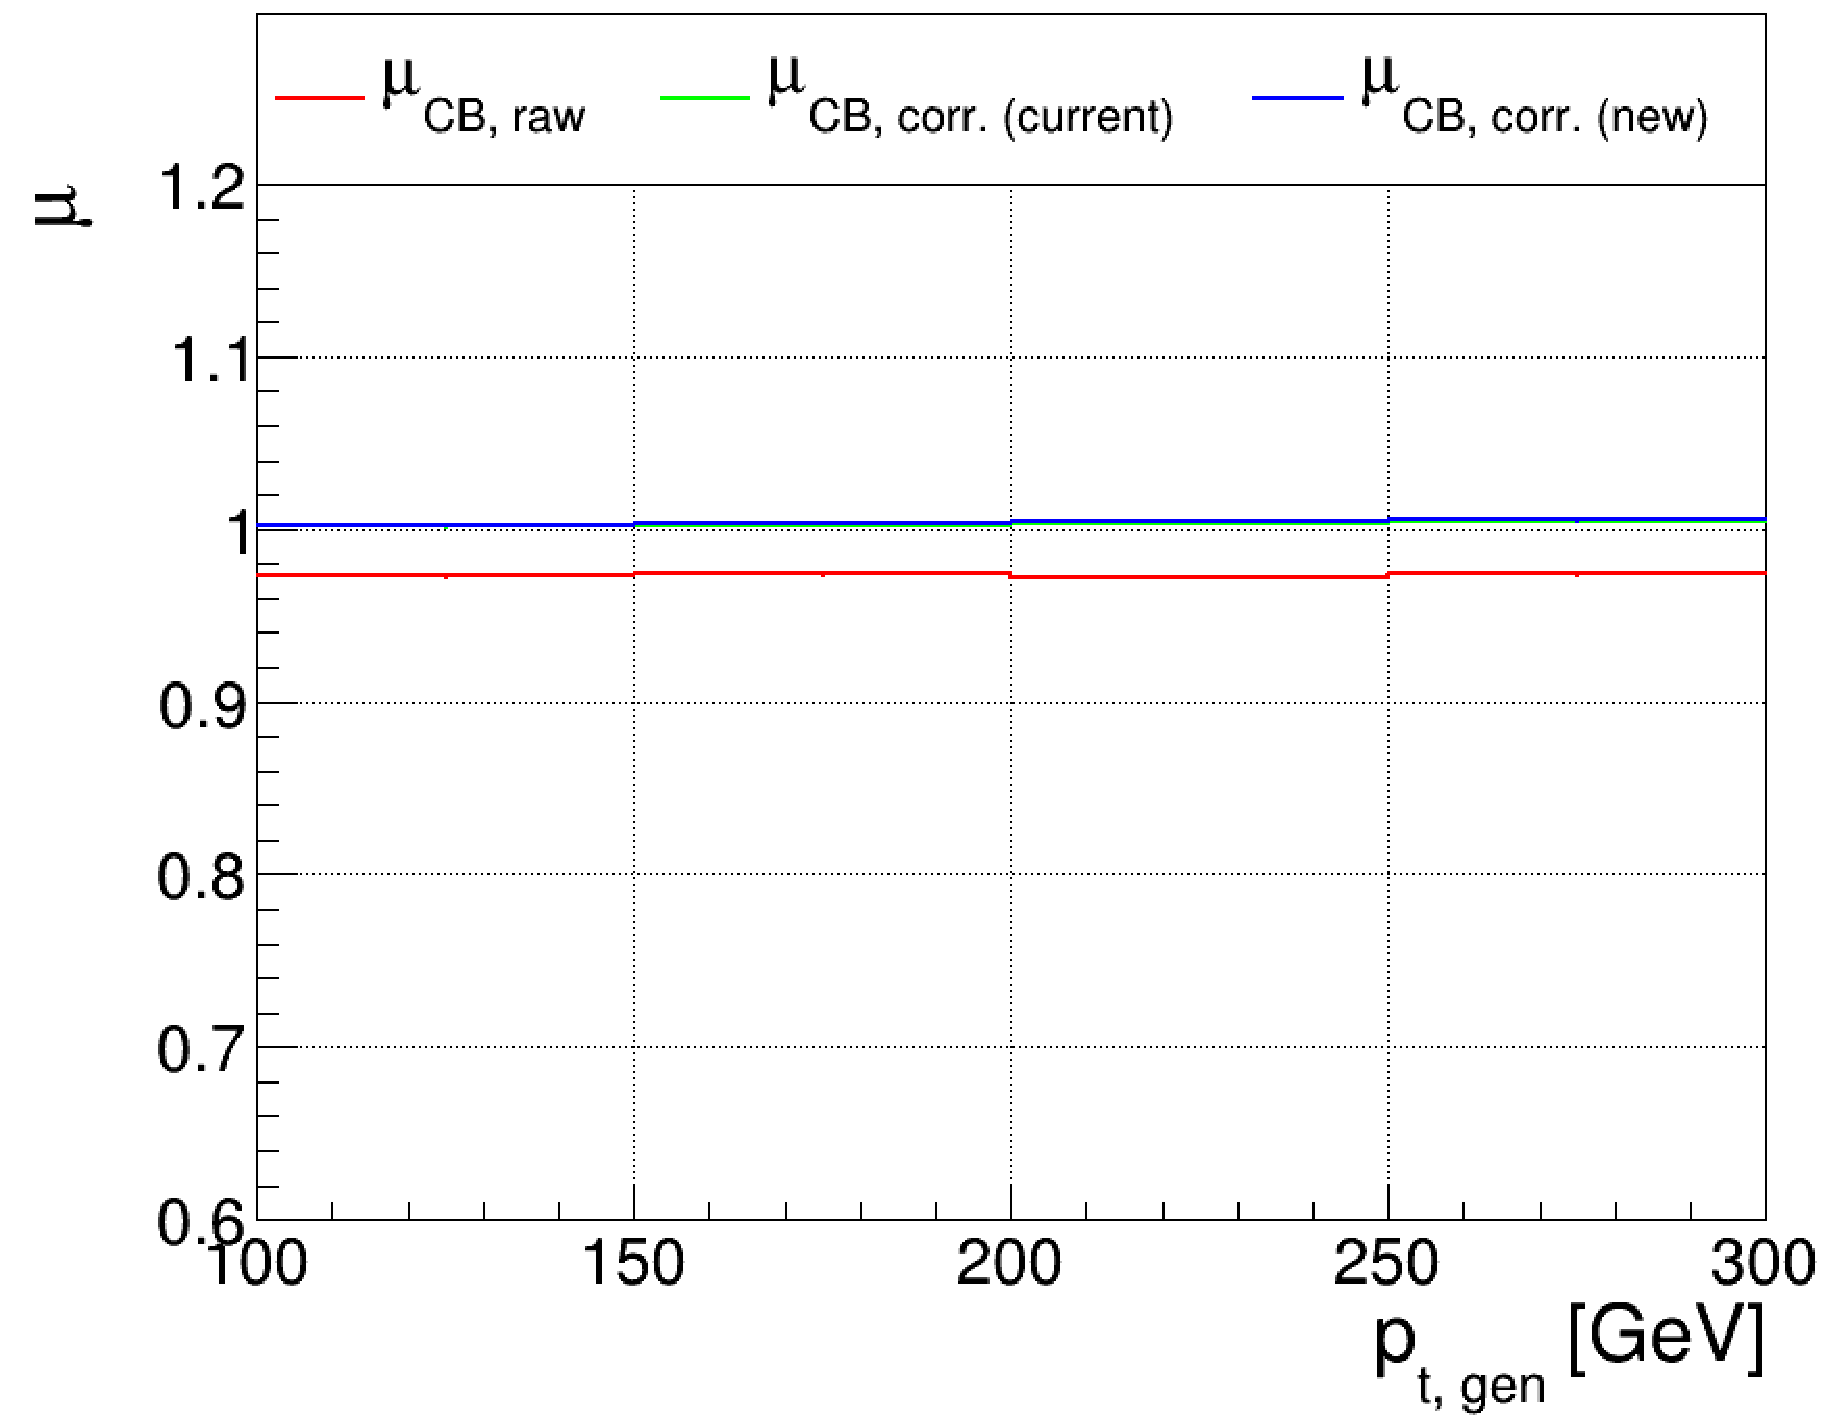
\includegraphics[width=0.495\textwidth]{./ECAL_plots/plotsNoPU/EE/pdf/FULL/GENPT/EEFULL_GENPT_0100_0300_MuOverBins.pdf}
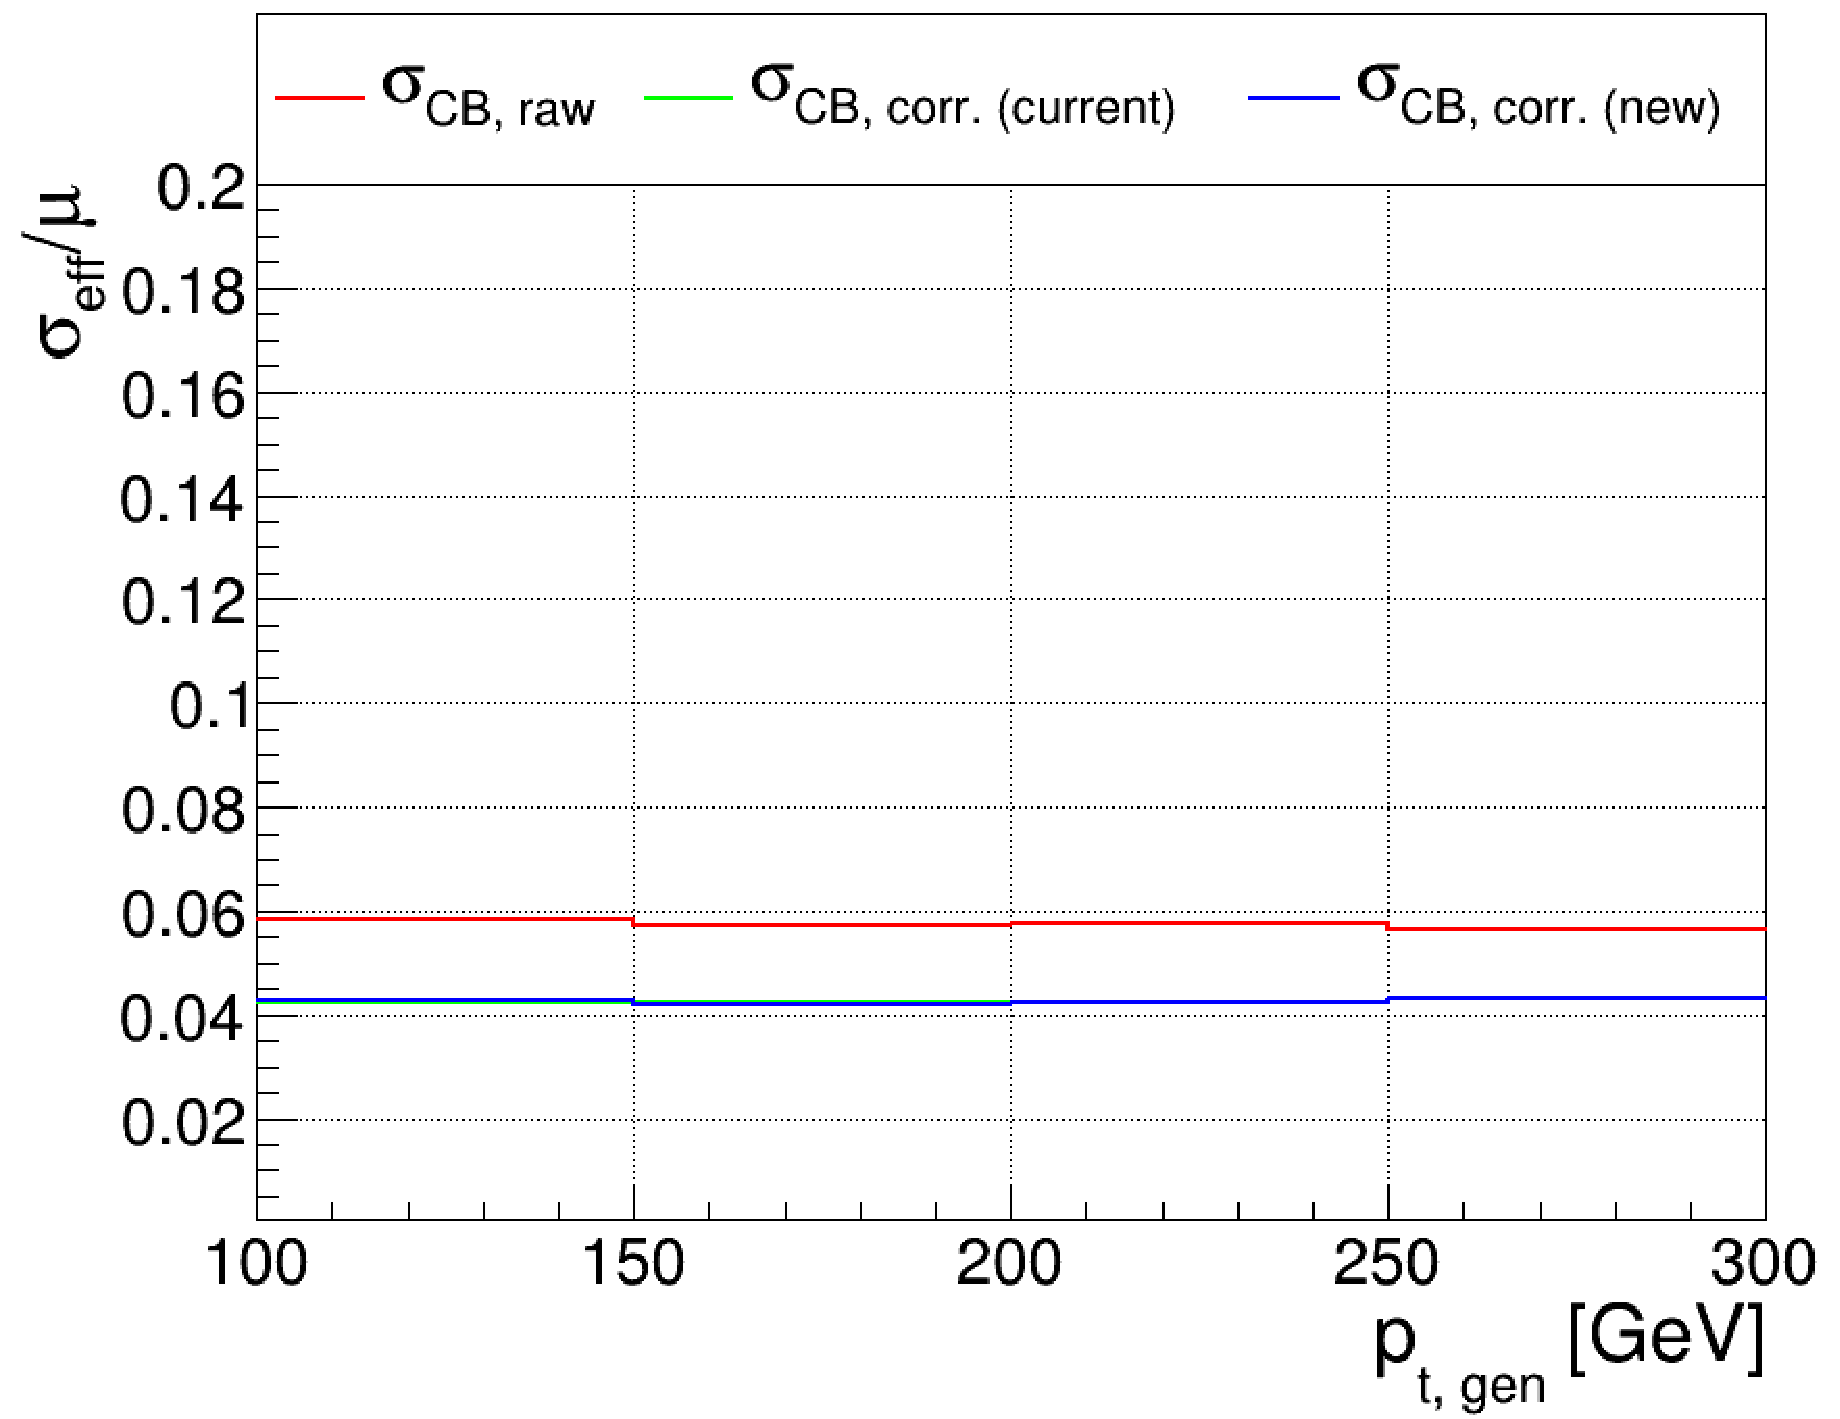
\includegraphics[width=0.495\textwidth]{./ECAL_plots/plotsNoPU/EE/pdf/FULL/GENPT/EEFULL_GENPT_0100_0300_EffSigmaOverBins.pdf}
%\caption{EE - Full Readout pt 100-300}
%\end{figure}
%\begin{figure}
\includegraphics[width=0.495\textwidth]{./ECAL_plots/plotsNoPU/EE/pdf/FULL/GENETA/EEFULL_GENETA_0100_0300_MuOverBins.pdf}
\includegraphics[width=0.495\textwidth]{./ECAL_plots/plotsNoPU/EE/pdf/FULL/GENETA/EEFULL_GENETA_0005_0020_EffSigmaOverBins.pdf}
\caption{EE - Full Readout pt 100-300}
\end{figure}





\begin{figure}
\includegraphics[width=0.495\textwidth]{./plots_pdf/ECAL_plots/plotsNoPU/EE/pdf/ZS/GENPT/EEZS_GENPT_0000_0006_MuOverBins.pdf}
\includegraphics[width=0.495\textwidth]{./plots_pdf/ECAL_plots/plotsNoPU/EE/pdf/ZS/GENPT/EEZS_GENPT_0000_0006_EffSigmaOverBins.pdf}

\includegraphics[width=0.495\textwidth]{./plots_pdf/ECAL_plots/plotsNoPU/EE/pdf/ZS/GENETA/EEZS_GENETA_0000_0006_MuOverBins.pdf}
\includegraphics[width=0.495\textwidth]{./plots_pdf/ECAL_plots/plotsNoPU/EE/pdf/ZS/GENETA/EEZS_GENETA_0000_0006_EffSigmaOverBins.pdf}
\caption[$\mu$ ($\sigma_\mathrm{eff}$) vs \pt of PF ECAL cluster - EE ZS readout NoPU scenario]{Mean response (resolution) defined by Raw PF ECAL clusters (red), the calibration derived earlier in Ru\
n3 based on 126X (green), and the new correction from 2024 simulation sample based on 133X (blue).\pt 0--6\GeV in EE region ZS Readout NOPU scenario.}
\end{figure}

%% %\begin{figure}
%% \includegraphics[width=0.495\textwidth]{./plots_pdf/ECAL_plots/plotsNoPU/EE/pdf/ZS/GENPT/EEZS_GENPT_0006_0025_MuOverBins.pdf}
%% \includegraphics[width=0.495\textwidth]{./plots_pdf/ECAL_plots/plotsNoPU/EE/pdf/ZS/GENPT/EEZS_GENPT_0006_0025_EffSigmaOverBins.pdf}
%% %\caption{EE - ZS Readout pt 6-25}
%% %\end{figure}
%% %\begin{figure}
%% \includegraphics[width=0.495\textwidth]{./plots_pdf/ECAL_plots/plotsNoPU/EE/pdf/ZS/GENETA/EEZS_GENETA_0006_0025_MuOverBins.pdf}
%% %\includegraphics[width=0.495\textwidth]{./ECAL_plots/plotsNoPU/EE/pdf/ZS/GENETA/EEZS_GENETA_0006_0025_EffSigmaOverBins.pdf}
%% \caption{EE - ZS Readout \pt 6-25}
%% \end{figure}




\begin{figure}
\includegraphics[width=0.495\textwidth]{./plots_pdf/ECAL_plots/plotsPU/EE/FULL/pdf/GENPT/EEFULL_GENPT_0005_0020_MuOverBins.pdf}
\includegraphics[width=0.495\textwidth]{./plots_pdf/ECAL_plots/plotsPU/EE/FULL/pdf/GENPT/EEFULL_GENPT_0005_0020_EffSigmaOverBins.pdf}
\includegraphics[width=0.495\textwidth]{./plots_pdf/ECAL_plots/plotsPU/EE/FULL/pdf/GENPT/EEFULL_GENPT_0020_0100_MuOverBins.pdf}
\includegraphics[width=0.495\textwidth]{./plots_pdf/ECAL_plots/plotsPU/EE/FULL/pdf/GENPT/EEFULL_GENPT_0020_0100_EffSigmaOverBins.pdf}
\includegraphics[width=0.495\textwidth]{./plots_pdf/ECAL_plots/plotsPU/EE/FULL/pdf/GENPT/EEFULL_GENPT_0100_0300_MuOverBins.pdf}
\includegraphics[width=0.495\textwidth]{./plots_pdf/ECAL_plots/plotsPU/EE/FULL/pdf/GENPT/EEFULL_GENPT_0100_0300_EffSigmaOverBins.pdf}

\caption [$\mu$ ($\sigma_\mathrm{eff}$) vs \pt of PF ECAL cluster - EE full readout PU scenario]{Mean response (resolution) defined by Raw PF ECAL clusters (red), the calibration derived earlier in Ru\
n3 based on 126X (green), and the new correction from 2024 simulation sample based on 133X (blue). (top) low \pt, (middle) mid \pt, (bottom) high \pt in EE region full readout PU scenario.}
\label{fig:PU_EEFULL_pt}
\end{figure}


\begin{figure}
\includegraphics[width=0.495\textwidth]{./plots_pdf/ECAL_plots/plotsPU/EE/FULL/pdf/GENETA/EEFULL_GENETA_0005_0020_MuOverBins.pdf}
\includegraphics[width=0.495\textwidth]{./plots_pdf/ECAL_plots/plotsPU/EE/FULL/pdf/GENETA/EEFULL_GENETA_0005_0020_EffSigmaOverBins.pdf}
\includegraphics[width=0.495\textwidth]{./plots_pdf/ECAL_plots/plotsPU/EE/FULL/pdf/GENETA/EEFULL_GENETA_0020_0100_MuOverBins.pdf}
\includegraphics[width=0.495\textwidth]{./plots_pdf/ECAL_plots/plotsPU/EE/FULL/pdf/GENETA/EEFULL_GENETA_0020_0100_EffSigmaOverBins.pdf}
\includegraphics[width=0.495\textwidth]{./plots_pdf/ECAL_plots/plotsPU/EE/FULL/pdf/GENETA/EEFULL_GENETA_0100_0300_MuOverBins.pdf}
\includegraphics[width=0.495\textwidth]{./plots_pdf/ECAL_plots/plotsPU/EE/FULL/pdf/GENETA/EEFULL_GENETA_0100_0300_EffSigmaOverBins.pdf}


\caption [$\mu$ ($\sigma_\mathrm{eff}$) vs $\eta$ of PF ECAL cluster - EE Full readout PU scenario]{Mean response (resolution) defined by Raw PF ECAL clusters (red), the calibration derived earlier in\
 Run3 based on 126X (green), and the new correction from 2024 simulation sample based on 133X (blue). (top) low $\eta$, (middle) mid $\eta$, (bottom) high $\eta$ in EE region Full readout PU scenario.}
\label{fig:PU_EEFULL_eta}
\end{figure}

\begin{figure}
\includegraphics[width=0.495\textwidth]{./plots_pdf/ECAL_plots/plotsPU/EE/ZS/pdf/GENPT/EEZS_GENPT_0000_0006_MuOverBins.pdf}
\includegraphics[width=0.495\textwidth]{./plots_pdf/ECAL_plots/plotsPU/EE/ZS/pdf/GENPT/EEZS_GENPT_0000_0006_EffSigmaOverBins.pdf}

\includegraphics[width=0.495\textwidth]{./plots_pdf/ECAL_plots/plotsPU/EE/ZS/pdf/GENETA/EEZS_GENETA_0000_0006_MuOverBins.pdf}
\includegraphics[width=0.495\textwidth]{./plots_pdf/ECAL_plots/plotsPU/EE/ZS/pdf/GENETA/EEZS_GENETA_0000_0006_EffSigmaOverBins.pdf}

\caption[$\mu$ ($\sigma_\mathrm{eff}$) vs. \pt of PF ECAL cluster - EE ZS readout PU scenario]{Mean response (resolution) defined by raw PF ECAL clusters (red), the calibration derived earlier in Run~3 based on 126X (green), and the new correction from the 2024 simulation sample based on 133X (blue).\pt 0--6\GeV in EE region ZS readout PU scenario.}
\label{fig:PU_EEZS}
\end{figure}

%% %\begin{figure}
%% \includegraphics[width=0.495\textwidth]{./plots_pdf/ECAL_plots/plotsPU/EE/ZS/pdf/GENPT/EEZS_GENPT_0006_0025_MuOverBins.pdf}
%% \includegraphics[width=0.495\textwidth]{./plots_pdf/ECAL_plots/plotsPU/EE/ZS/pdf/GENPT/EEZS_GENPT_0006_0025_EffSigmaOverBins.pdf}
%% %\caption{EE - ZS Readout pt 6-25}
%% %\end{figure}
%% %\begin{figure}
%% \includegraphics[width=0.495\textwidth]{./plots_pdf/ECAL_plots/plotsPU/EE/ZS/pdf/GENETA/EEZS_GENETA_0006_0025_MuOverBins.pdf}
%% \caption{EE - ZS Readout \pt 6-25}
%% \end{figure}








HLT vs offline PF ECAL cluster

(connet to PF chapter where where we mentioned offline PF)

first for NoPU samples




%%%%%%%%%%%%%%%%%%%%%%%%%%%%%%%%%%%%%%%%%%%%%%%                                                                                                                                     
\begin{figure}
\includegraphics[width=0.495\textwidth]{./ECAL_plots/Prod6/NoPU/H_GenPi_Pt_vs_RespE.pdf}
%\caption{(PF cluster offline E / PFC online E) vs pt}
\includegraphics[width=0.495\textwidth]{./ECAL_plots/Prod6/NoPU/H_GenPi_Eta_vs_RespE.pdf}
\caption{(PF cluster offline E / PFC online E)}
\end{figure}

\begin{figure}
\includegraphics[width=0.495\textwidth]{./ECAL_plots/Prod6/NoPU/H_GenPi_Pt_vs_RespCE.pdf}
%\caption{(PF cluster offline E corrected / PFC online E corrected) vs pt}
\includegraphics[width=0.495\textwidth]{./ECAL_plots/Prod6/NoPU/H_GenPi_Eta_vs_RespCE.pdf}
\caption{(PF cluster offline E corrected / PFC online E corrected)}
\end{figure}                                                                                                                                                                       
%%%%%%%%%%%%%%%%%%%%%%%%%%%%%%%%%%%%%%%%%%%%%%%%                                                                                                                                    


Second for PUU samples
\begin{figure}
\includegraphics[width=0.495\textwidth]{./plots_pdf/ECAL_plots/Prod6/PU/H_GenPi_Pt_vs_RespE.pdf}
%\caption{(PF cluster offline E / PFC online E) vs pt}                                                                 
\includegraphics[width=0.495\textwidth]{./plots_pdf/ECAL_plots/Prod6/PU/H_GenPi_Eta_vs_RespE.pdf}
\caption{(PF cluster offline E / PFC online E)}
\label{fig:PU_ECAL_Offline_vs_Online_E}
\end{figure}

\begin{figure}
\includegraphics[width=0.495\textwidth]{./plots_pdf/ECAL_plots/Prod6/PU/H_GenPi_Pt_vs_RespCE.pdf}
%\caption{(PF cluster offline E corrected / PFC online E corrected) vs pt}                                             
\includegraphics[width=0.495\textwidth]{./plots_pdf/ECAL_plots/Prod6/PU/H_GenPi_Eta_vs_RespCE.pdf}
\caption{(PF cluster offline E corrected / PFC online E corrected)}
\label{fig:PU_ECAL_Offline_vs_Online_CE}
\end{figure}       

B
